\documentclass[11pt,a4paper]{article}

% Configuration de l'encodage et support du français
\usepackage[T1]{fontenc}
\usepackage[utf8]{inputenc}
\usepackage[french]{babel}
\usepackage{lmodern}  % Police avec un meilleur support des accents
\usepackage{eurosym}  % Pour le symbole euro et autres symboles européens

% Mise en page
\usepackage[top=2.5cm,bottom=2.5cm,left=2.5cm,right=2.5cm]{geometry}
\usepackage{fancyhdr}
\usepackage{titlesec}
\usepackage{titletoc}

% Mathématiques et sciences
\usepackage{amsmath}
\usepackage{amssymb}
\usepackage{physics}
\usepackage{siunitx}

% Graphiques et couleurs
\usepackage{tikz}
\usepackage{pgfplots}
\pgfplotsset{compat=newest}
\usepackage{xcolor}

% Tableaux et listes
\usepackage{booktabs}
\usepackage{array}
\usepackage{enumitem}
\usepackage{multirow}

% Images et figures
\usepackage{graphicx}
\usepackage{float}
\usepackage{wrapfig}
\usepackage{subcaption}

% Code et algorithmes
\usepackage{listings}
\usepackage{algorithm2e}
\usepackage[newfloat]{minted}

% Configuration de listings pour les accents
\lstset{
    inputencoding=utf8,
    extendedchars=true,
    literate=%
    {é}{{\'{e}}}1
    {è}{{\`{e}}}1
    {ê}{{\^{e}}}1
    {ë}{{\¨{e}}}1
    {à}{{\`{a}}}1
    {â}{{\^{a}}}1
    {î}{{\^{i}}}1
    {ï}{{\¨{i}}}1
    {ô}{{\^{o}}}1
    {ù}{{\`{u}}}1
    {û}{{\^{u}}}1
    {ü}{{\¨{u}}}1
    {ç}{{\c{c}}}1
}

% Références et bibliographie
\usepackage[hidelinks]{hyperref}
\usepackage{cleveref}
\usepackage[style=alphabetic,backend=biber]{biblatex}
\addbibresource{references.bib}

% Définition des couleurs personnalisées
\definecolor{primaryblue}{HTML}{1f77b4}
\definecolor{secondaryblue}{HTML}{7BA6C4}
\definecolor{accentorange}{HTML}{ff7f0e}
\definecolor{backgroundgray}{HTML}{f7f7f7}
\definecolor{tertiarygreen}{HTML}{2ca02c}

% Configuration des titres
\titleformat{\section}
{\color{primaryblue}\Large\bfseries}
{\thesection}{1em}{}[\titlerule]

\titleformat{\subsection}
{\color{secondaryblue}\large\bfseries}
{\thesubsection}{1em}{}

% Configuration des en-têtes et pieds de page
\pagestyle{fancy}
\fancyhf{}
\fancyhead[L]{\textit{Parallélisation temporelle du système de Lorenz}}
\fancyhead[R]{\thepage}
\fancyfoot[C]{\textit{\today}}

% Configuration des listings de code
\lstset{
    basicstyle=\ttfamily\small,
    breaklines=true,
    commentstyle=\color{green!60!black},
    keywordstyle=\color{blue},
    stringstyle=\color{red},
    numbers=left,
    numberstyle=\tiny\color{gray},
    frame=single,
    backgroundcolor=\color{backgroundgray},
    tabsize=4
}

% Paramètres de l'algorithme
\SetAlgoLined
\SetKwInput{KwInput}{Entrées}
\SetKwInput{KwOutput}{Sorties}

% Configuration de pgfplots
\pgfplotsset{
    every axis/.append style={
        line width=1pt,
        tick style={thin},
        grid style={thin,gray!30},
        grid=major,
        legend style={font=\small}
    }
}

% Titre du document
\title{%
    \textcolor{primaryblue}{\Huge\textbf{Parallélisation temporelle pour la résolution\\du système de Lorenz}}\\[1cm]
    \textcolor{secondaryblue}{\Large Une approche avec l'algorithme Parareal}\\[1cm]
    \vspace{0.5cm}
    \Large\textcolor{tertiarygreen}{
        Elonm AHOUANYE\\
        Yanel AÏNA\\[0.5cm]
        École Nationale Supérieure de Génie Mathématique et Modélisation\\
        (ENSGMM Abomey)\\[0.5cm]
        \large\textit{Supervisé par}\\
        \normalsize{Dr. DANDOGBESSI Bruno}\\
    }
}

\date{\today}

\begin{document}

\maketitle
\thispagestyle{empty}

\clearpage
\begin{abstract}
Ce document présente une étude approfondie de la parallélisation temporelle appliquée au système de Lorenz modifié pour une particule active guidée par sa mémoire. Nous explorons l'implémentation de l'algorithme Parareal comme alternative à la méthode RK4 séquentielle traditionnelle, en mettant l'accent sur les aspects théoriques et pratiques de cette approche novatrice.
\end{abstract}

\setcounter{tocdepth}{2}
\tableofcontents
\clearpage

% Introduction
% Introduction slides

\begin{frame}{Contexte physique : particules actives guidées par la mémoire}
    \begin{itemize}
        \item Les systèmes de particules actives : un domaine de la physique moderne
        \item Les gouttes "marcheuses" sur un bain liquide vibrant
        \item Interaction avec les ondes auto-générées
        \item Mémoire ondulatoire guidant le mouvement
    \end{itemize}
\end{frame}

\begin{frame}{Du système physique au modèle mathématique}
    \begin{itemize}
        \item Équation de trajectoire intégro-différentielle :
        \begin{equation}
            \ddot{x}_d + \dot{x}_d = F_{self} + F_{bias}
        \end{equation}
        \item Force du champ d'ondes auto-généré :
        \begin{equation}
            F_{self} = -R\int_{-\infty}^t W'(x_d(t)-x_d(s)) e^{-\frac{t-s}{\tau}} ds
        \end{equation}
    \end{itemize}
\end{frame}

\begin{frame}{Émergence du système de Lorenz}
    \begin{itemize}
        \item Simplification avec $W(x) = \cos(x)$
        \item Variables :
        \begin{align*}
            X &= \dot{x}_d \quad \text{(vitesse)} \\
            Y &= F_{self} \quad \text{(force de mémoire)} \\
            Z &= R\int_{-\infty}^t \cos(x_d(t)-x_d(s)) e^{-\frac{t-s}{\tau}} ds
        \end{align*}
        \item Système de Lorenz modifié :
        \begin{equation*}
        \begin{cases}
            \dot{X} = Y - X \\
            \dot{Y} = -\frac{1}{\tau} Y + XZ \\
            \dot{Z} = R - \frac{1}{\tau} Z - XY
        \end{cases}
        \end{equation*}
    \end{itemize}
\end{frame}

\begin{frame}{Problématique}
    \begin{itemize}
        \item \textbf{Défis de la résolution numérique :}
        \begin{itemize}
            \item Non-linéarité : termes de couplage $XZ$ et $XY$
            \item Sensibilité aux conditions initiales
            \item Échelles multiples : paramètre $\tau$
        \end{itemize}
        \vspace{0.5cm}
        \item \textbf{Objectifs :}
        \begin{itemize}
            \item Résolution séquentielle avec RK4
            \item Parallélisation temporelle avec l'algorithme Parareal
            \item Analyse des performances et de la précision
        \end{itemize}
    \end{itemize}
\end{frame}
\clearpage

% Resolution rk4 
\section{Résolution numérique par la méthode RK4}

\subsection{Formulation pour le système de Lorenz}
La méthode RK4 s'applique au système de Lorenz en traitant simultanément les trois équations couplées. Pour un état $\mathbf{u} = (X, Y, Z)$, le système peut s'écrire sous la forme :

\begin{equation}
\frac{d\mathbf{u}}{dt} = \mathbf{f}(\mathbf{u}) = \begin{pmatrix}
Y - X \\
-\frac{1}{\tau}Y + XZ \\
R - \frac{1}{\tau}Z - XY
\end{pmatrix}
\end{equation}

\subsubsection{Calcul des coefficients}
Les coefficients $k_i$ de la méthode RK4 sont calculés comme suit :

\begin{align}
k_1 &= \mathbf{f}(t_n, \mathbf{u}_n) \\
k_2 &= \mathbf{f}(t_n + \frac{h}{2}, \mathbf{u}_n + \frac{h}{2}k_1) \\
k_3 &= \mathbf{f}(t_n + \frac{h}{2}, \mathbf{u}_n + \frac{h}{2}k_2) \\
k_4 &= \mathbf{f}(t_n + h, \mathbf{u}_n + hk_3)
\end{align}

où $h$ est le pas de temps et $\mathbf{u}_n$ est l'état du système au temps $t_n$.

\subsection{Implémentation}

\subsubsection{Structure du code}
Le solveur RK4 est implémenté comme une sous-routine Fortran qui prend en compte les spécificités du système de Lorenz :

\begin{lstlisting}[language=Fortran,caption=Implémentation RK4 pour le système de Lorenz]
module rk4_solver
    use types, only: dp
    implicit none

    type :: LorenzState
        real(dp) :: X, Y, Z
    end type LorenzState

contains
    subroutine solve_step(state, dt, tau, R)
        type(LorenzState), intent(inout) :: state
        real(dp), intent(in) :: dt, tau, R
        type(LorenzState) :: k1, k2, k3, k4, temp
        
        ! Calcul de k1
        k1%X = state%Y - state%X
        k1%Y = -state%Y/tau + state%X * state%Z
        k1%Z = R - state%Z/tau - state%X * state%Y
        
        ! Calcul de k2
        temp = state
        temp%X = state%X + dt*k1%X/2
        temp%Y = state%Y + dt*k1%Y/2
        temp%Z = state%Z + dt*k1%Z/2
        k2%X = temp%Y - temp%X
        k2%Y = -temp%Y/tau + temp%X * temp%Z
        k2%Z = R - temp%Z/tau - temp%X * temp%Y
        
        ! Calcul de k3
        temp%X = state%X + dt*k2%X/2
        temp%Y = state%Y + dt*k2%Y/2
        temp%Z = state%Z + dt*k2%Z/2
        k3%X = temp%Y - temp%X
        k3%Y = -temp%Y/tau + temp%X * temp%Z
        k3%Z = R - temp%Z/tau - temp%X * temp%Y
        
        ! Calcul de k4
        temp%X = state%X + dt*k3%X
        temp%Y = state%Y + dt*k3%Y
        temp%Z = state%Z + dt*k3%Z
        k4%X = temp%Y - temp%X
        k4%Y = -temp%Y/tau + temp%X * temp%Z
        k4%Z = R - temp%Z/tau - temp%X * temp%Y
        
        ! Mise à jour finale
        state%X = state%X + (dt/6)*(k1%X + 2*k2%X + 2*k3%X + k4%X)
        state%Y = state%Y + (dt/6)*(k1%Y + 2*k2%Y + 2*k3%Y + k4%Y)
        state%Z = state%Z + (dt/6)*(k1%Z + 2*k2%Z + 2*k3%Z + k4%Z)
    end subroutine solve_step
end module rk4_solver
\end{lstlisting}

\subsection{Analyse des résultats}


\subsubsection{Paramètres de simulation}
Les simulations ont été réalisées avec les paramètres suivants :

\begin{itemize}
    \item \textbf{Pas de temps} : $h = 0.01$
    \item \textbf{Durée totale} : $T = 100.0$
    \item \textbf{Amplitude des ondes} : $R = 2.5$
    \item \textbf{Conditions initiales} : $(X_0, Y_0, Z_0) = (1.0, 0.0, 0.0)$
\end{itemize}


% \subsubsection{Caractéristiques des différents régimes}
% \begin{itemize}
%     \item $\tau$ = 0.5 : Amortissement rapide des oscillations (État Non-Marcheur)
%     \item $\tau$ = 2.0 : Établissement d'états stationnaires symétriques (Marche Régulière)
%     \item $\tau$ = 5.0 : Oscillations périodiques avec motifs complexes (Marche Chaotique)
%     \item $\tau$ = 8.9 : Dynamique chaotique avec attracteur étrange (Oscillations avec Dérive)
% \end{itemize}


% \subsection{Analyse des régimes dynamiques}
En fonction du paramètre de mémoire $\tau$, le système présente différents comportements caractéristiques.

\subsubsection{État Non-Marcheur ($\tau$ = 0.5) }
Pour une faible valeur de $\tau$, le système converge rapidement vers un point fixe.

On peut également noter que la trajectoire converge rapidement vers l'origine (X → 0) et l'absence d'oscillations.

\begin{figure}[H]
    \centering
    \begin{subfigure}[b]{0.5\textwidth}
        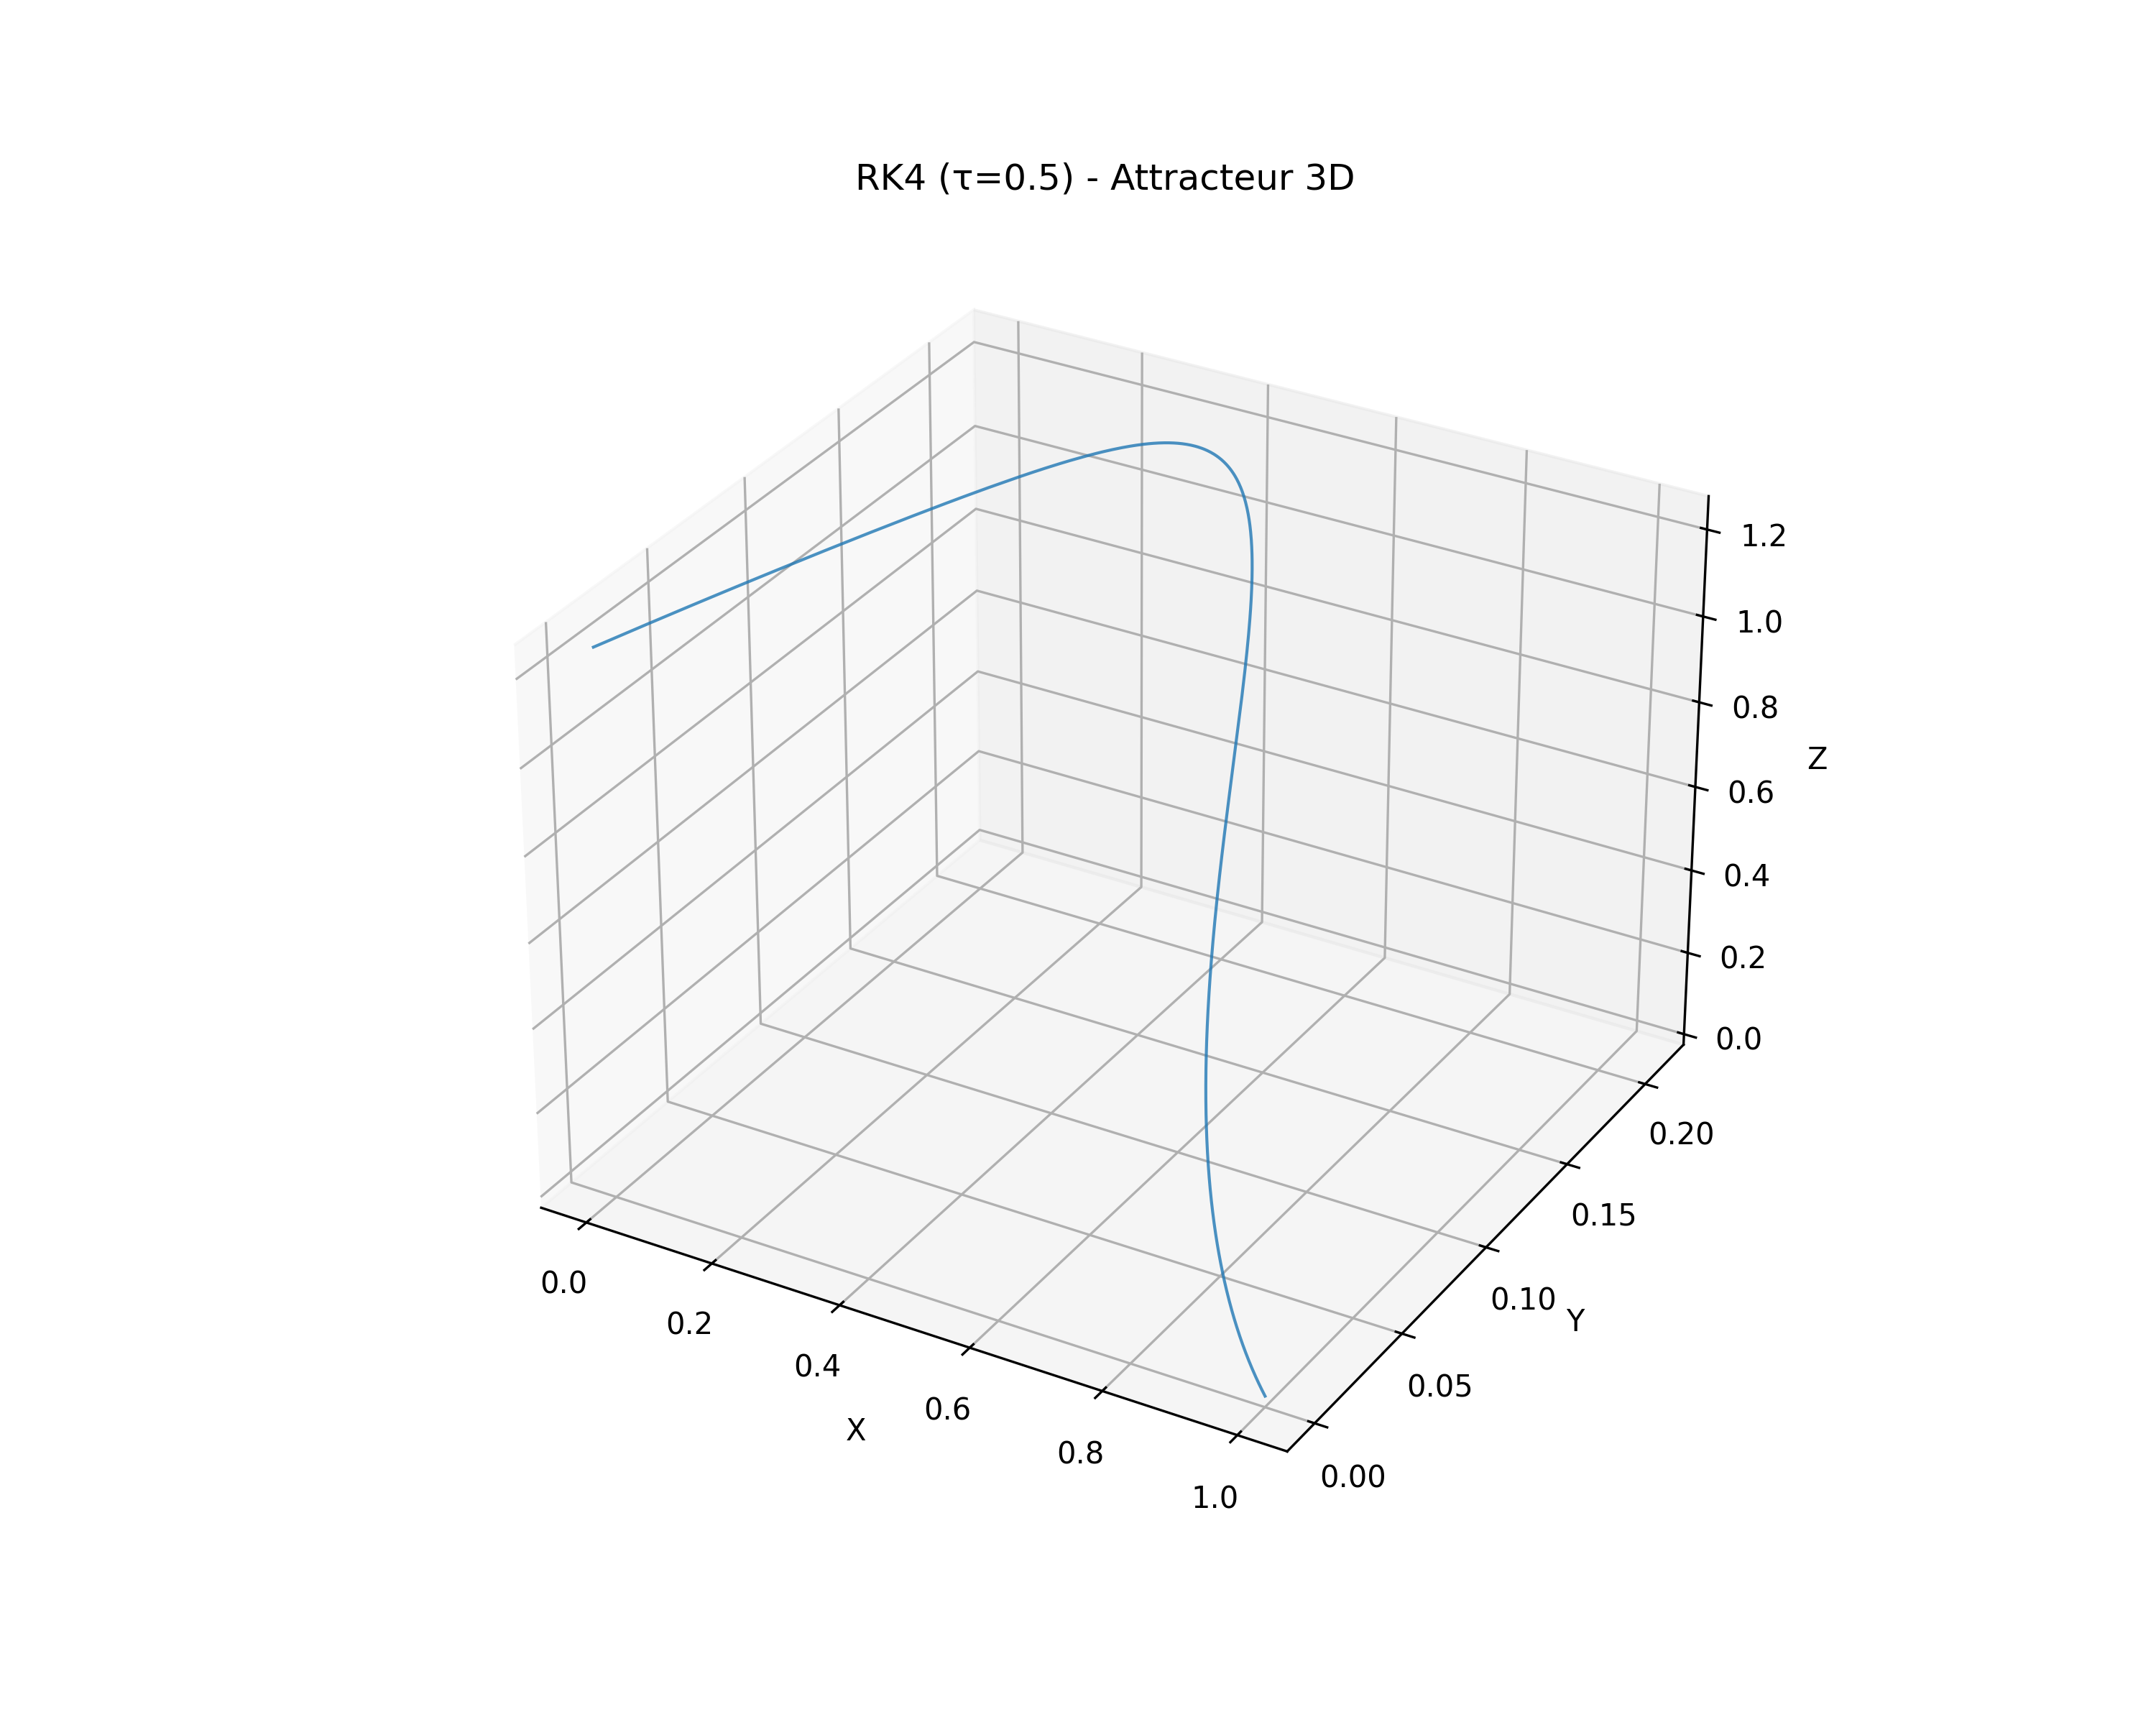
\includegraphics[width=\textwidth]{figures/rk4/rk4_tau0.5_3d}
        \caption{Trajectoire 3D}
    \end{subfigure}
    \begin{subfigure}[b]{0.4\textwidth}
        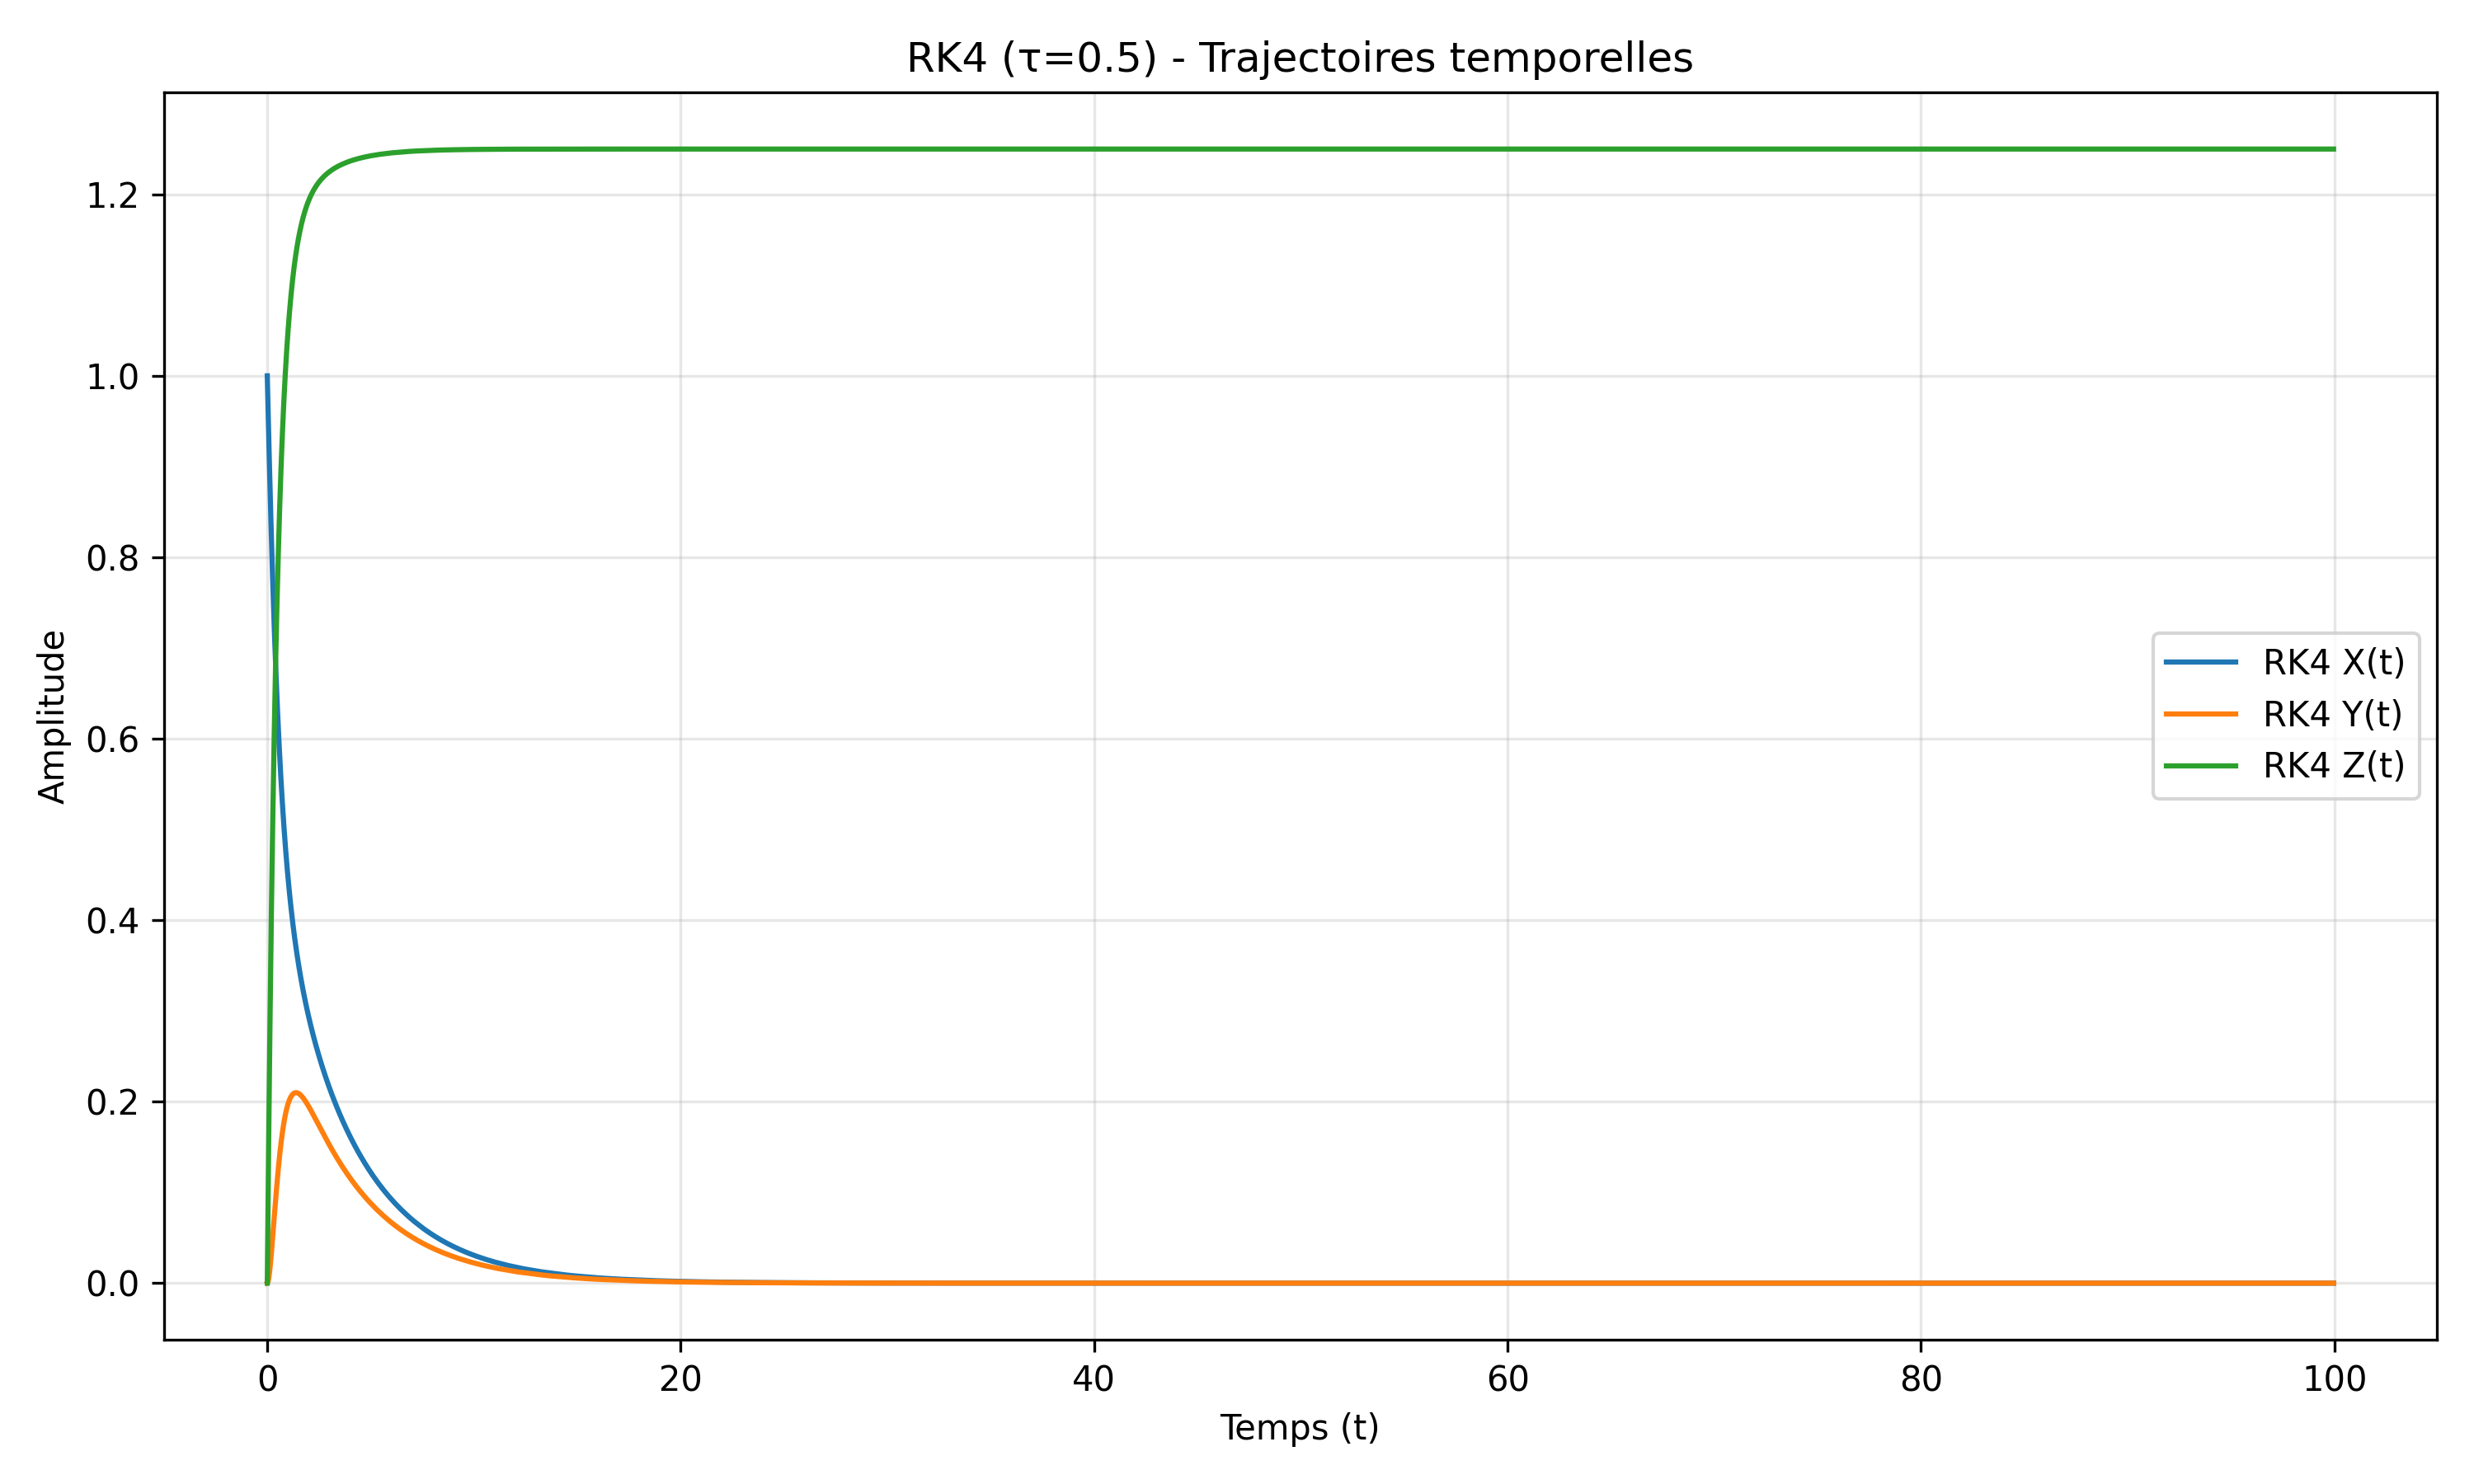
\includegraphics[width=\textwidth]{figures/rk4/rk4_tau0.5_time}
        \caption{Évolution temporelle : X converge rapidement vers zéro, Y et Z se stabilisent}
    \end{subfigure}
    \begin{subfigure}[b]{0.3\textwidth}
        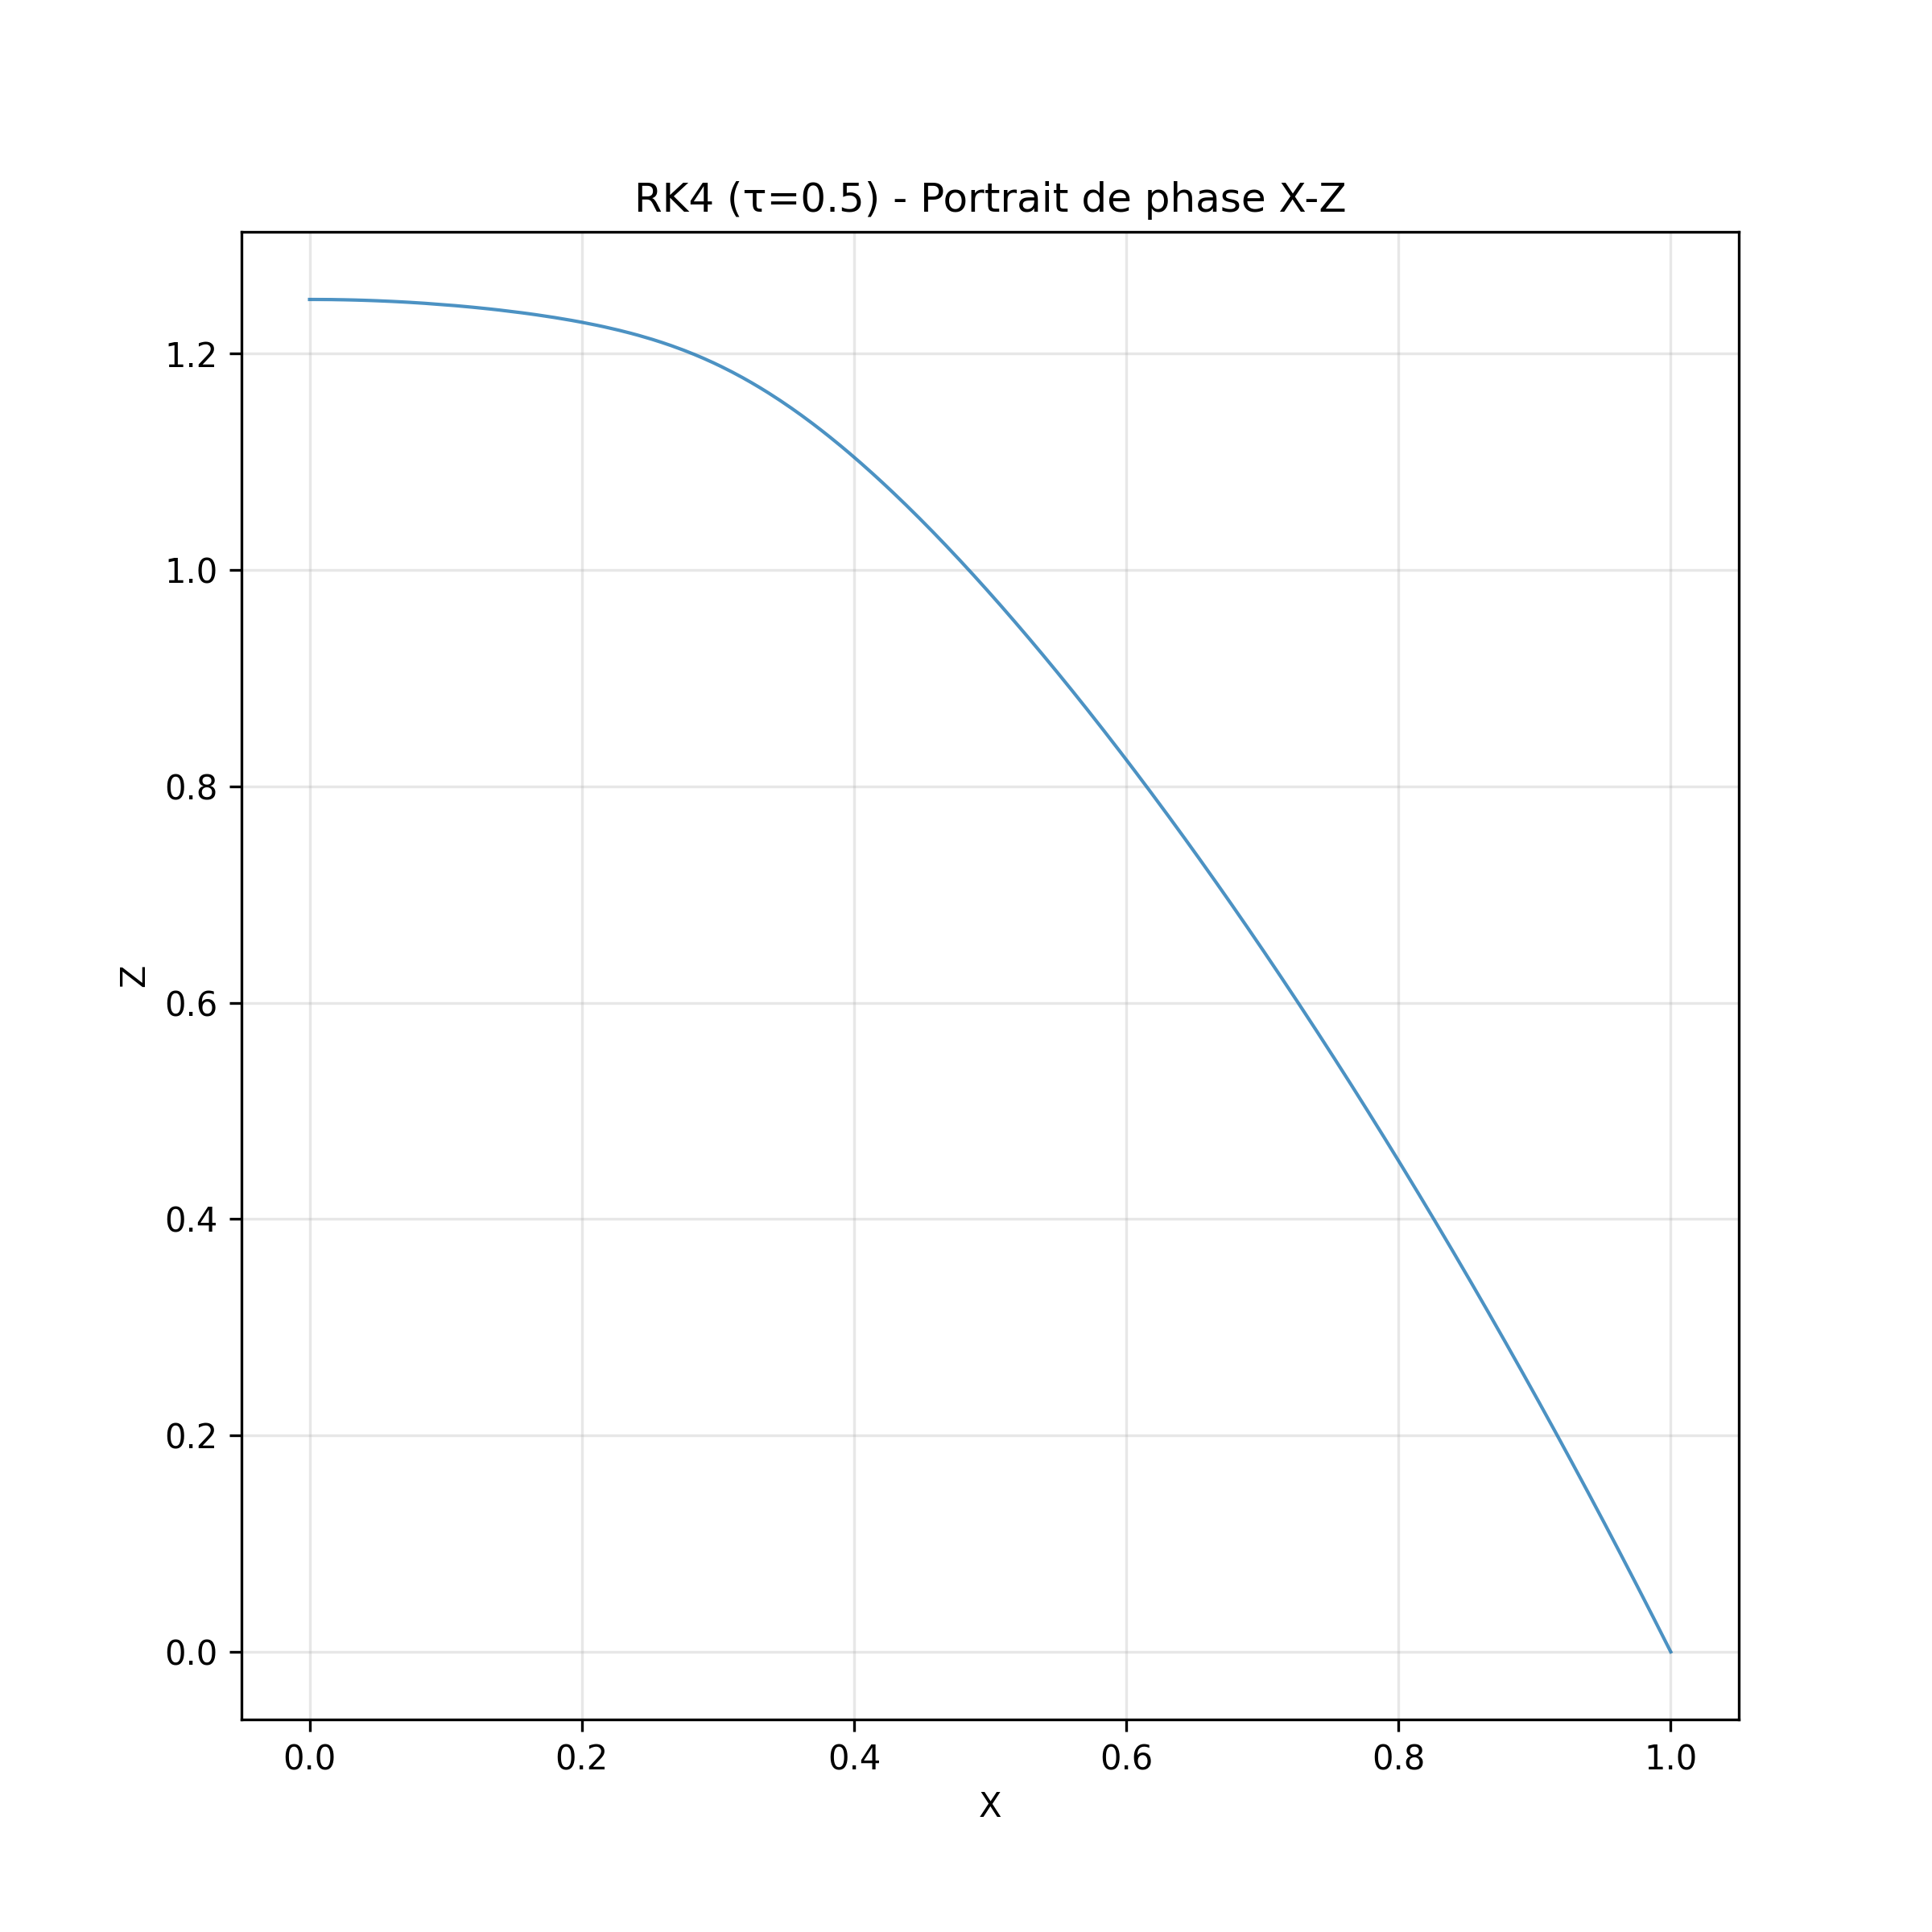
\includegraphics[width=\textwidth]{figures/rk4/rk4_tau0.5_phase}
        \caption{Portrait de phase}
    \end{subfigure}
    \caption{Dynamique pour $\tau$ = 0.5 : convergence vers un point fixe}
    \label{fig:rk4_tau0.5}
\end{figure}

\subsubsection{Marche Régulière ($\tau$ = 2.0)}
À $\tau$ = 2.0, le système présente des états stationnaires stables non triviaux.

En effet, on peut observer une stabilisation de la trajectoire autour de X non nulle et constante. 
\begin{figure}[H]
    \centering
    \begin{subfigure}[b]{0.5\textwidth}
        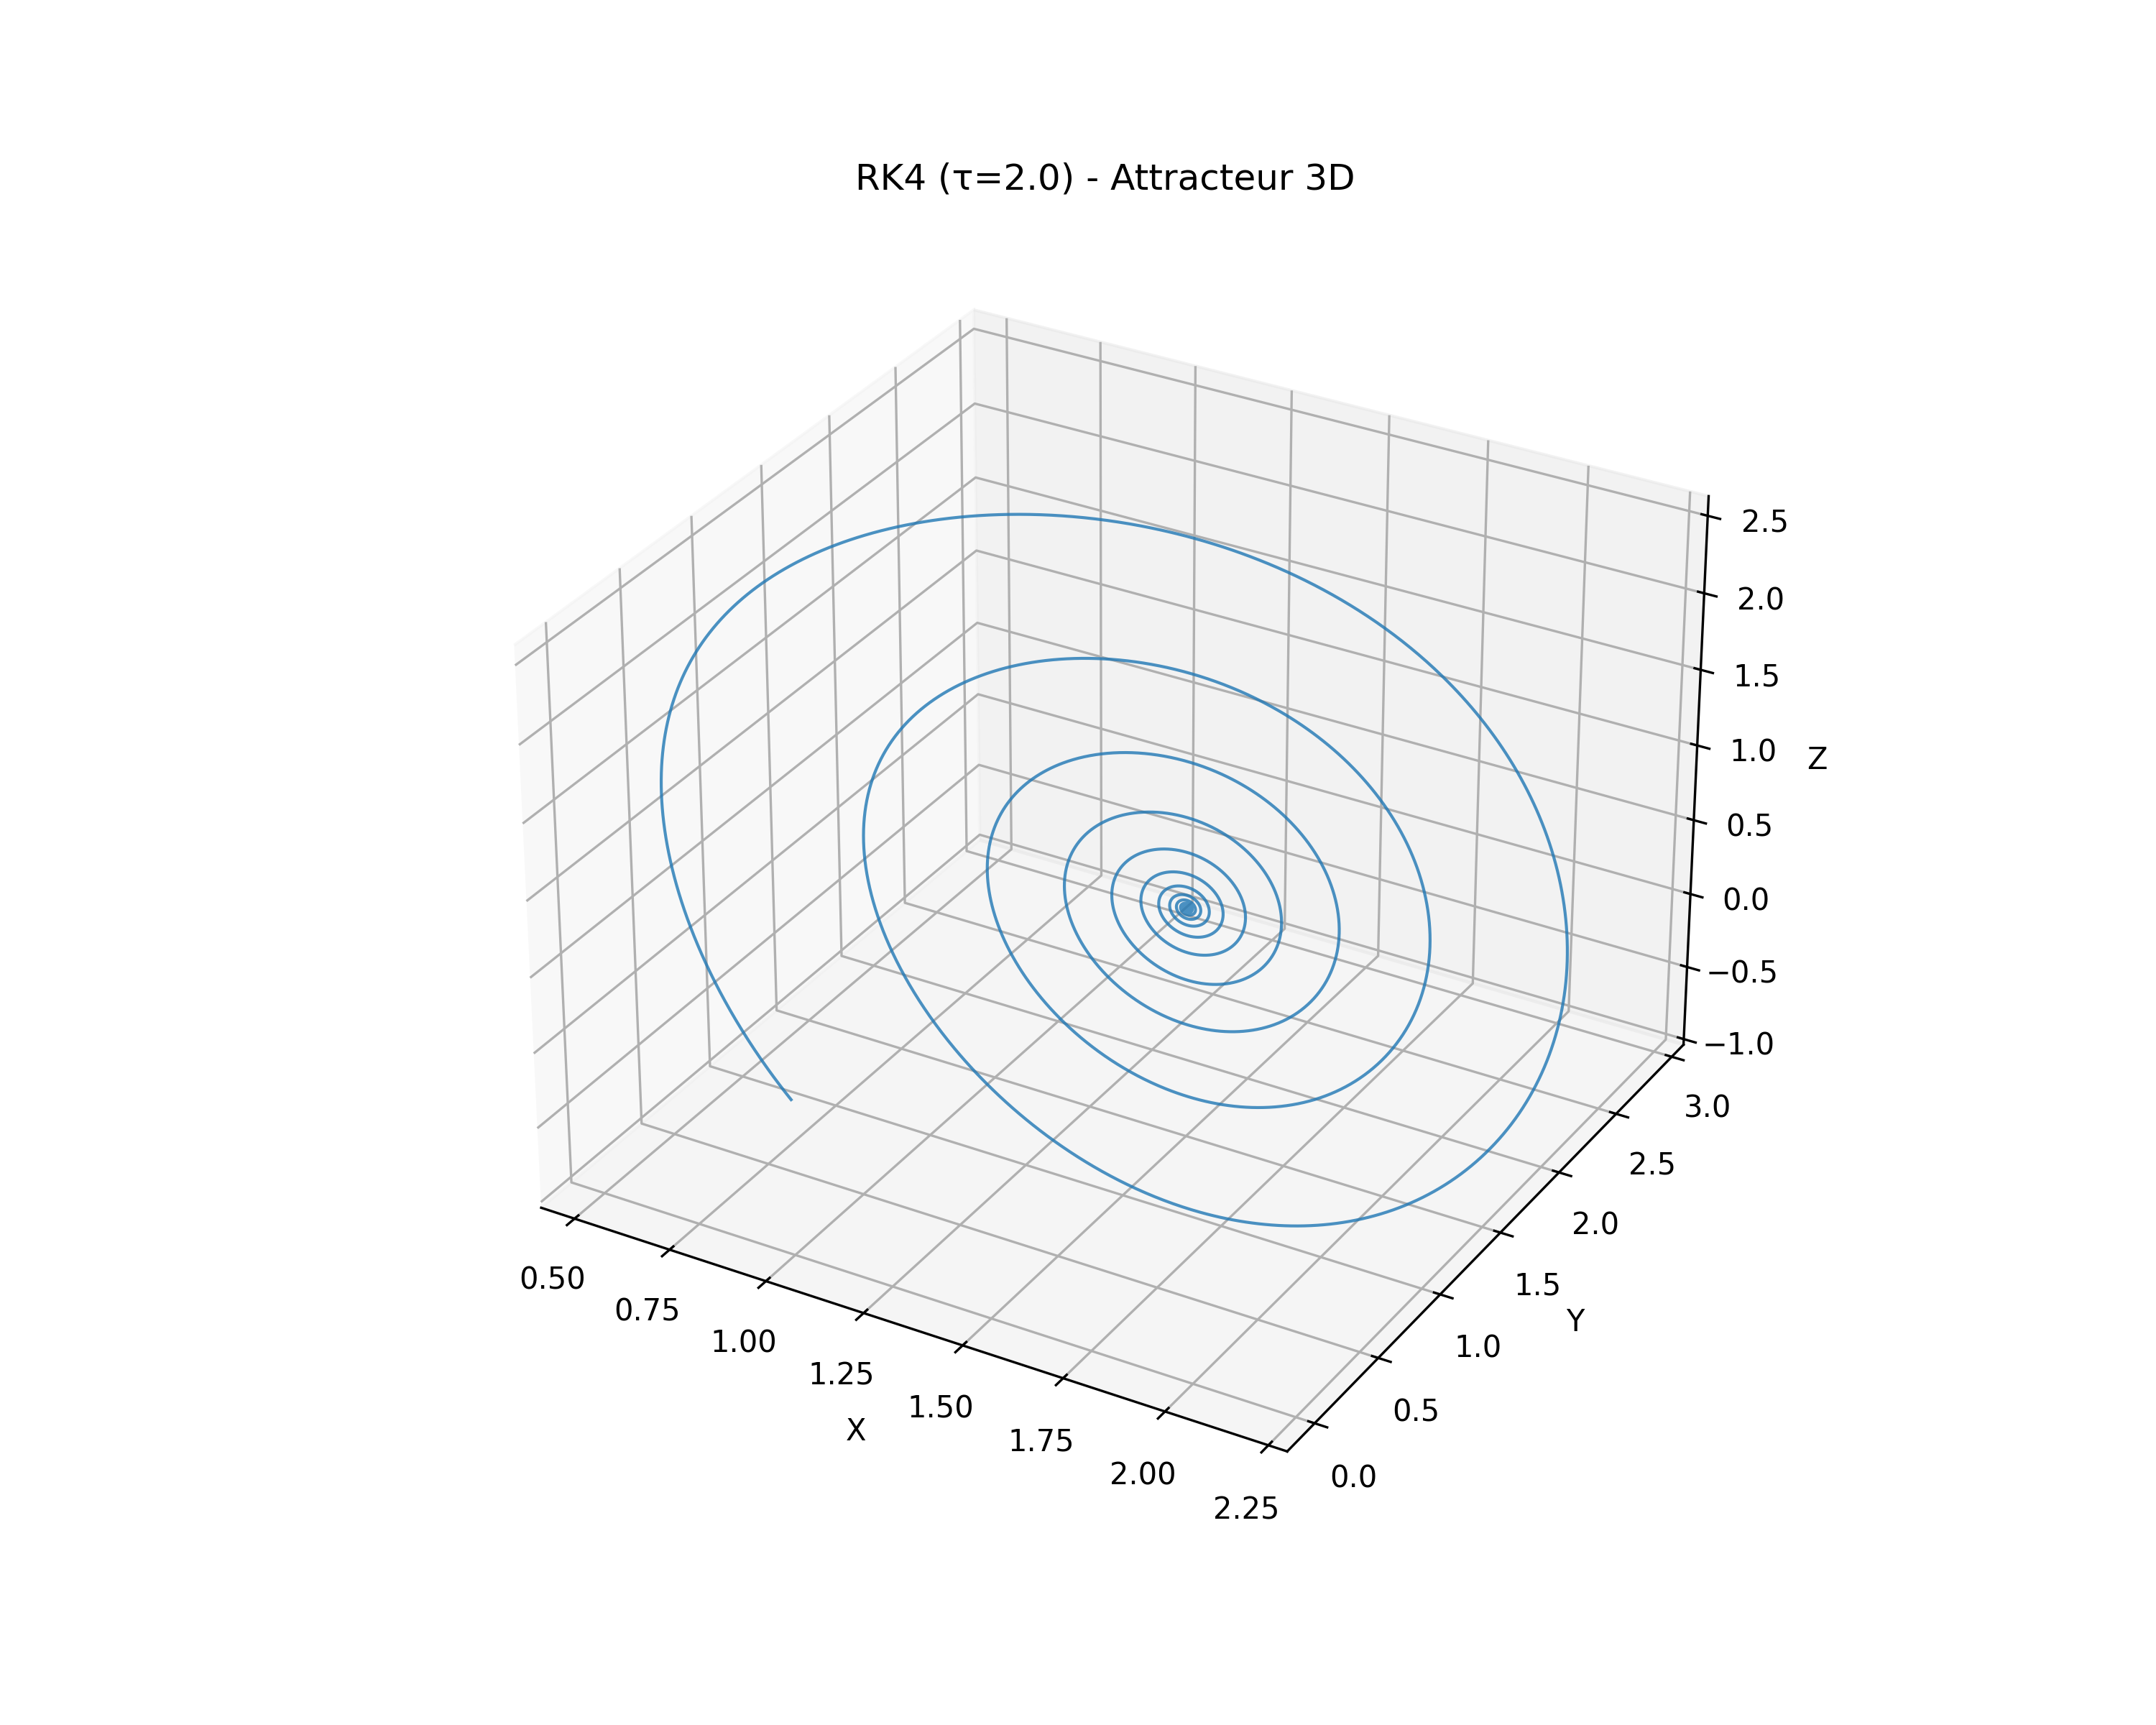
\includegraphics[width=\textwidth]{figures/rk4/rk4_tau2.0_3d}
        \caption{Trajectoire 3D : Trajectoire convergeant vers un point fixe non trivial}
    \end{subfigure}
    \begin{subfigure}[b]{0.4\textwidth}
        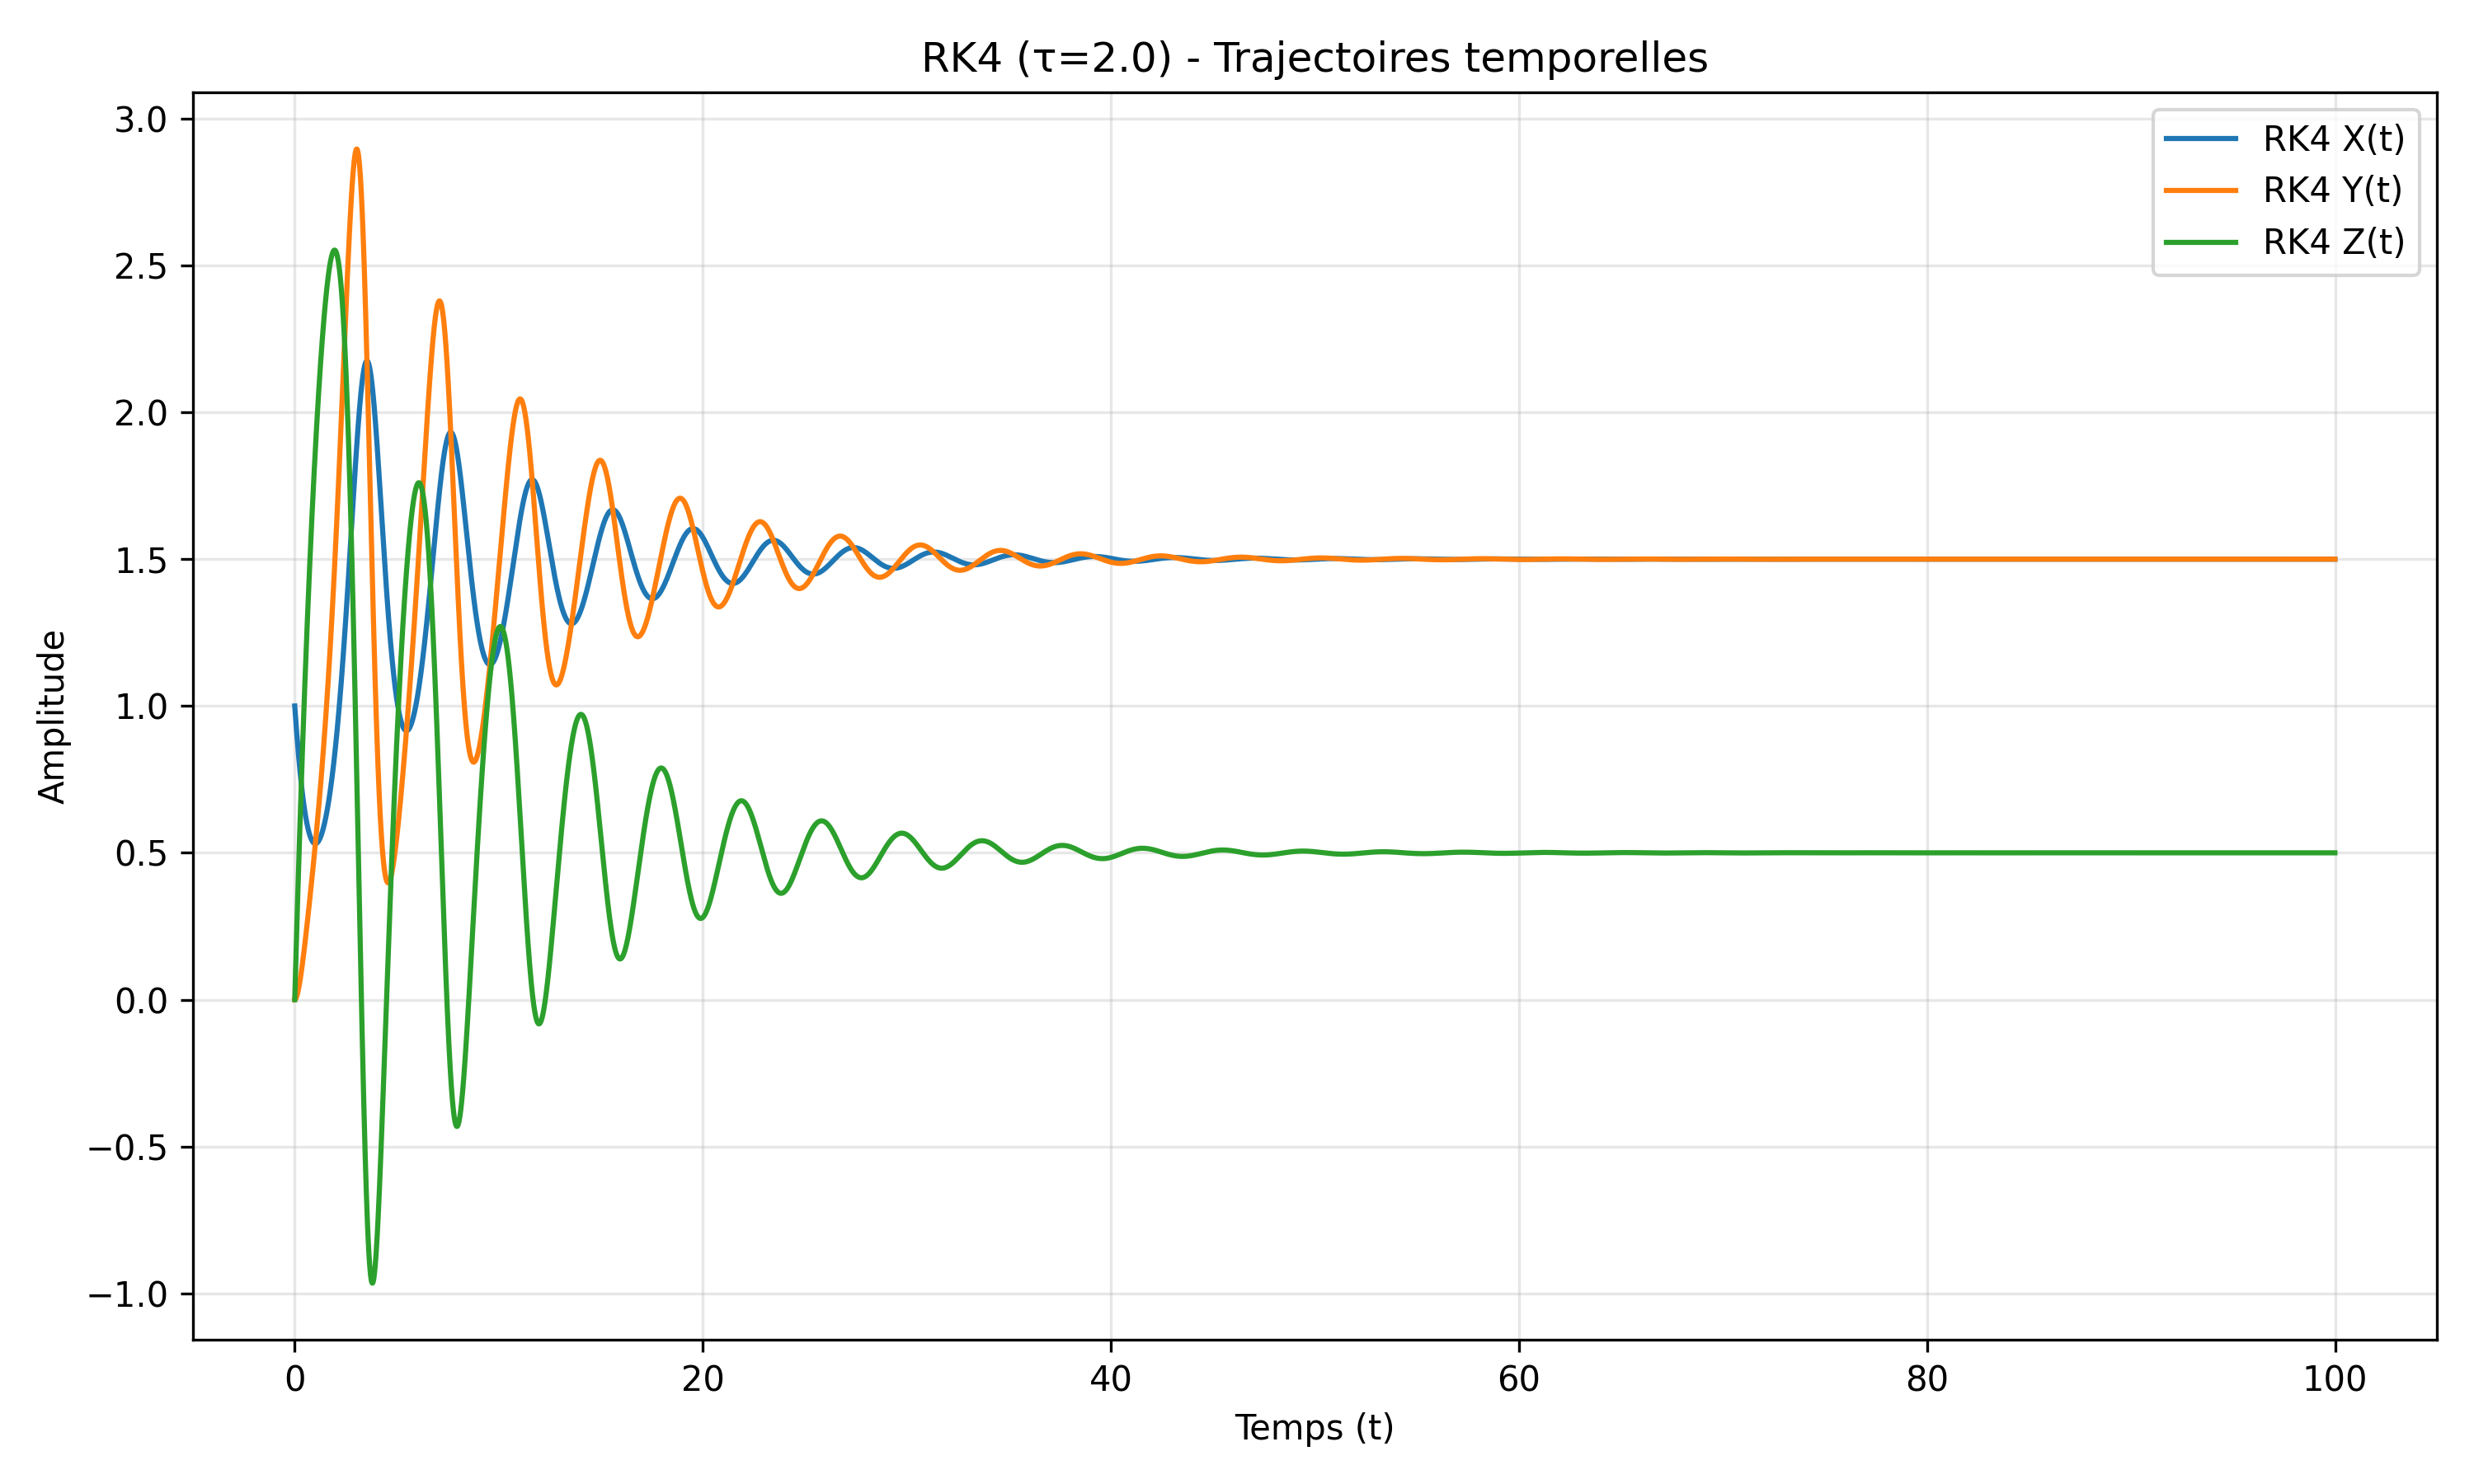
\includegraphics[width=\textwidth]{figures/rk4/rk4_tau2.0_time}
        \caption{Évolution temporelle : X et Y se stabilisent à des valeurs non-nulles constantes, Z reste stable}
    \end{subfigure}
    \begin{subfigure}[b]{0.3\textwidth}
        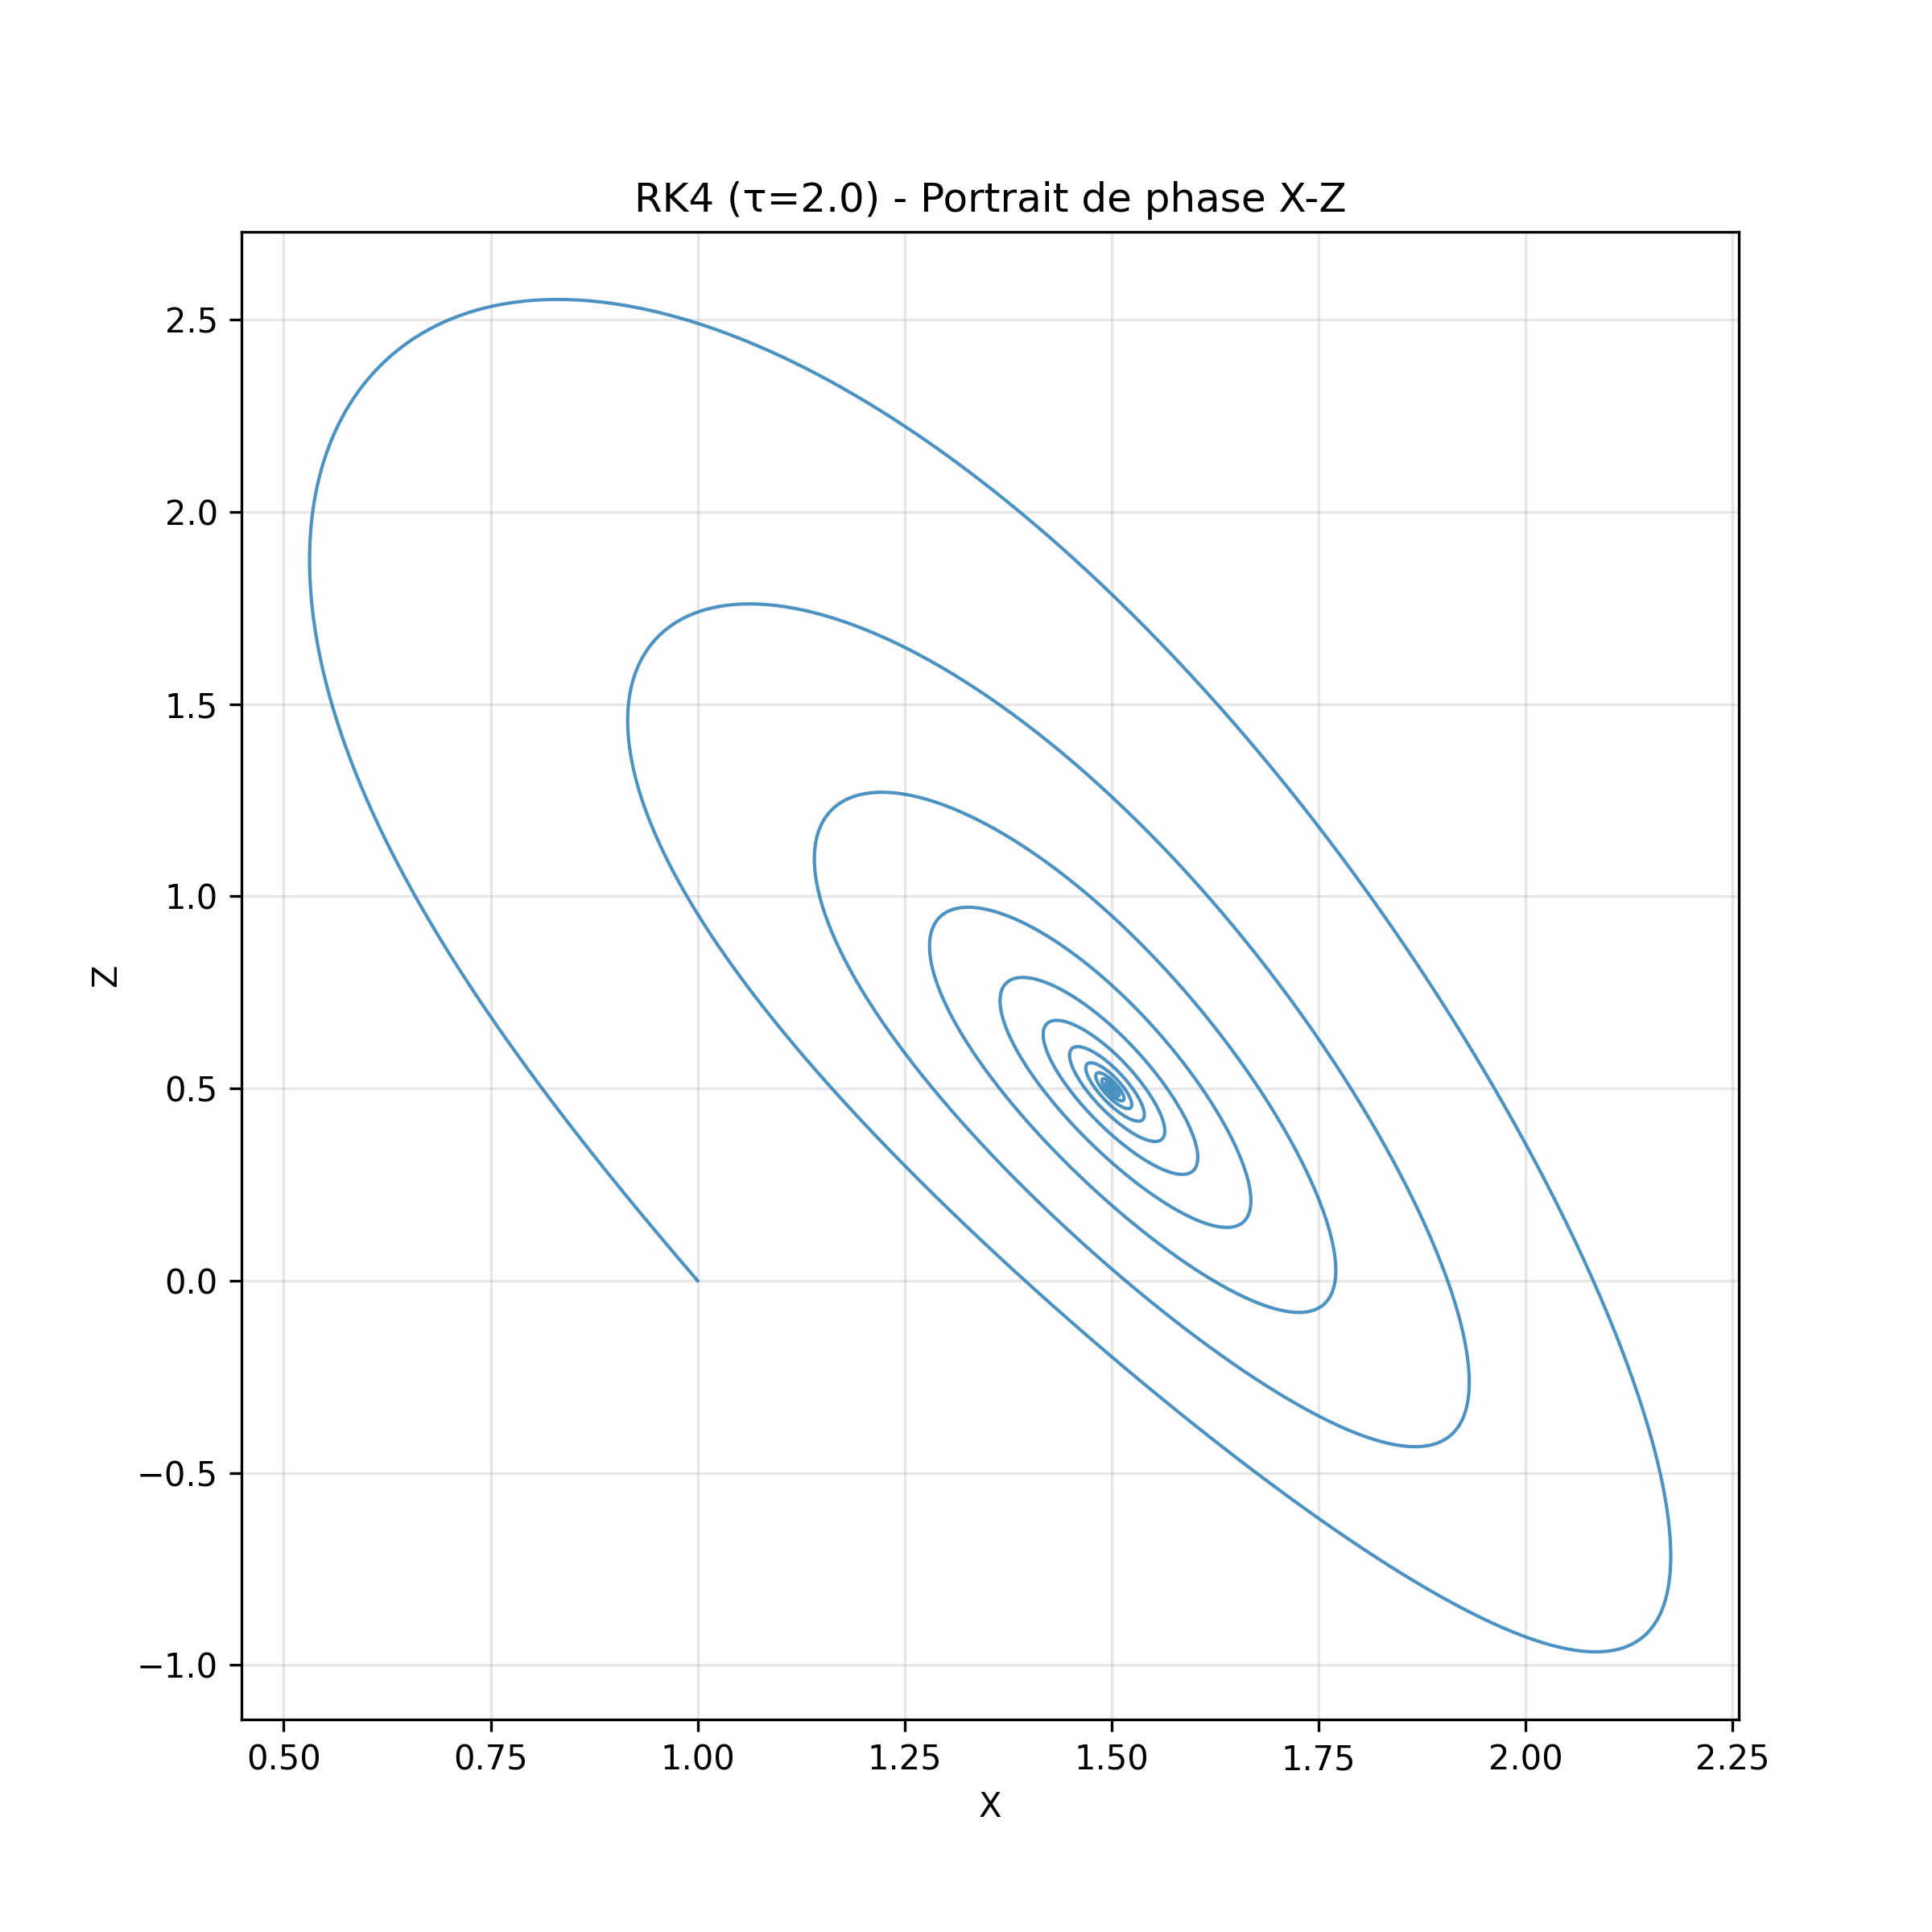
\includegraphics[width=\textwidth]{figures/rk4/rk4_tau2.0_phase}
        \caption{Portrait de phase}
    \end{subfigure}
    \caption{Dynamique pour $\tau$ = 2.0 : états stationnaires stables}
    \label{fig:rk4_tau2.0}
\end{figure}

\subsubsection{Marche Chaotique ($\tau$ = 5.0)}
À $\tau$ = 5.0, on observe l'apparition d'oscillations complexes.

Aucun motif régulier ou périodique n'est observable clairement dans la dynamique du système.
\begin{figure}[H]
    \centering
    \begin{subfigure}[b]{0.5\textwidth}
        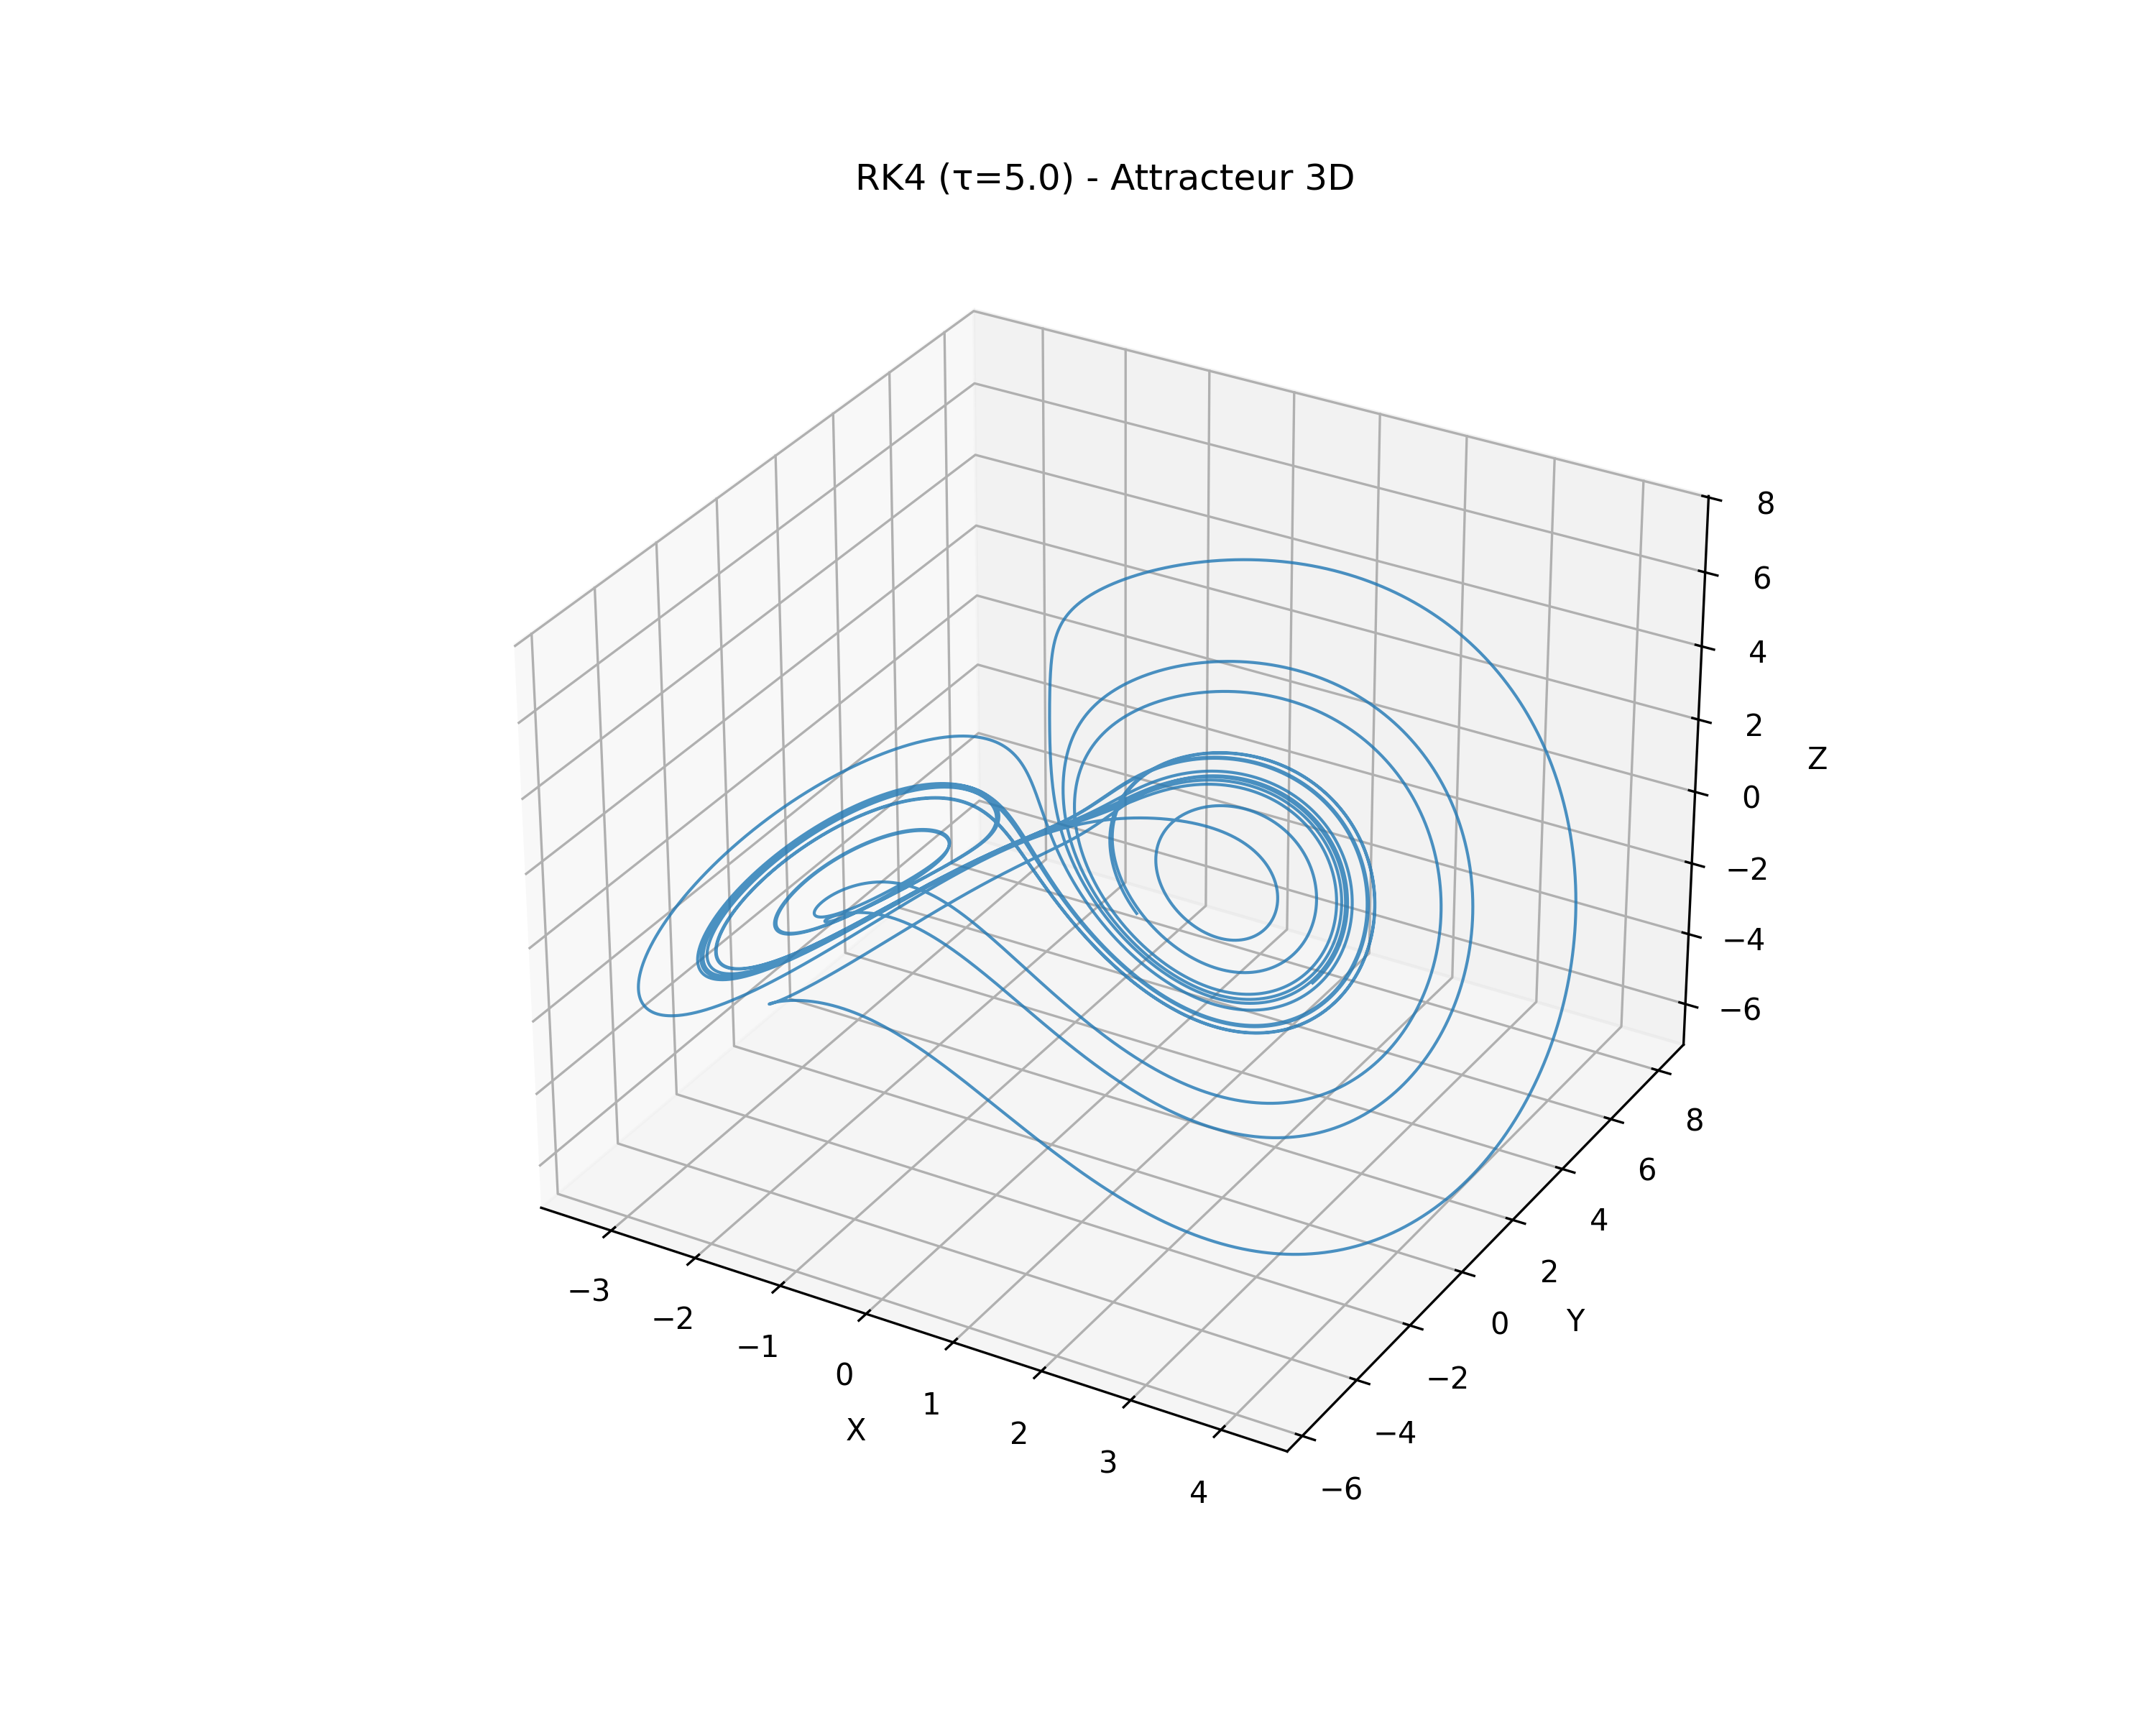
\includegraphics[width=\textwidth]{figures/rk4/rk4_tau5.0_3d}
        \caption{Trajectoire 3D : Attracteur étrange tridimensionnel avec structure complexe}
    \end{subfigure}
    \begin{subfigure}[b]{0.4\textwidth}
        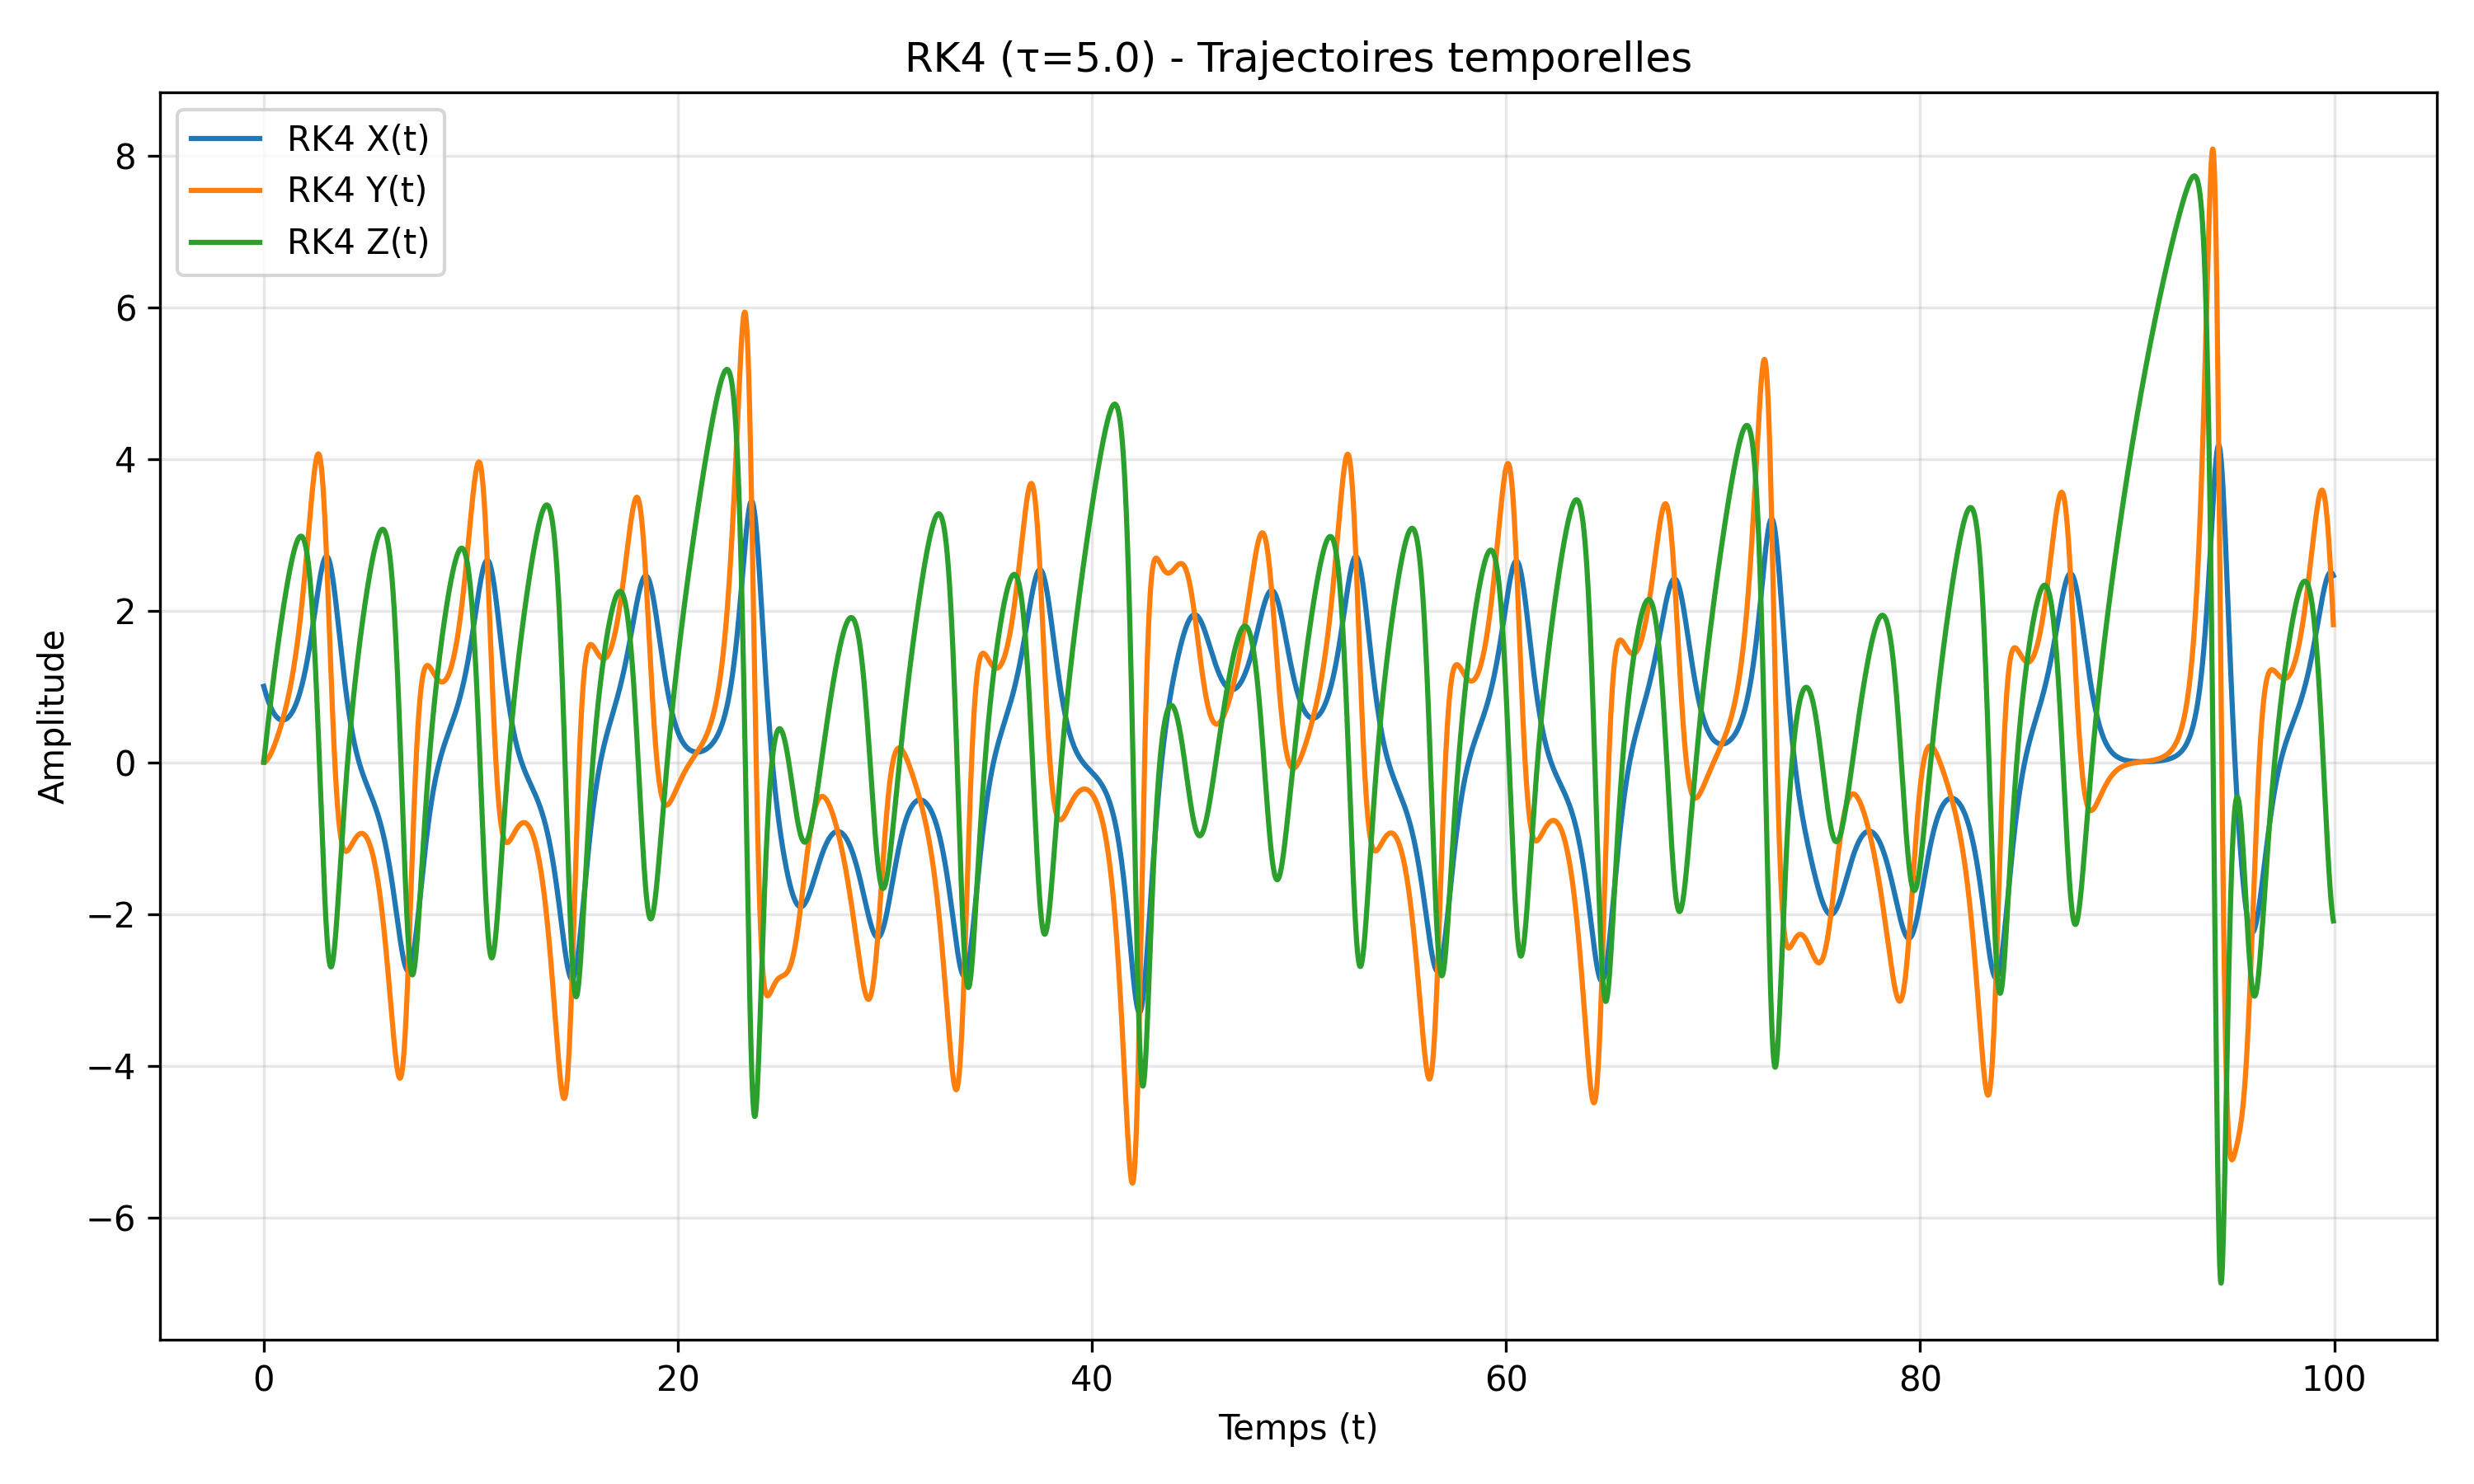
\includegraphics[width=\textwidth]{figures/rk4/rk4_tau5.0_time}
        \caption{Évolution temporelle : Fortes oscillations irrégulières de toutes les variables }
    \end{subfigure}
    \begin{subfigure}[b]{0.3\textwidth}
        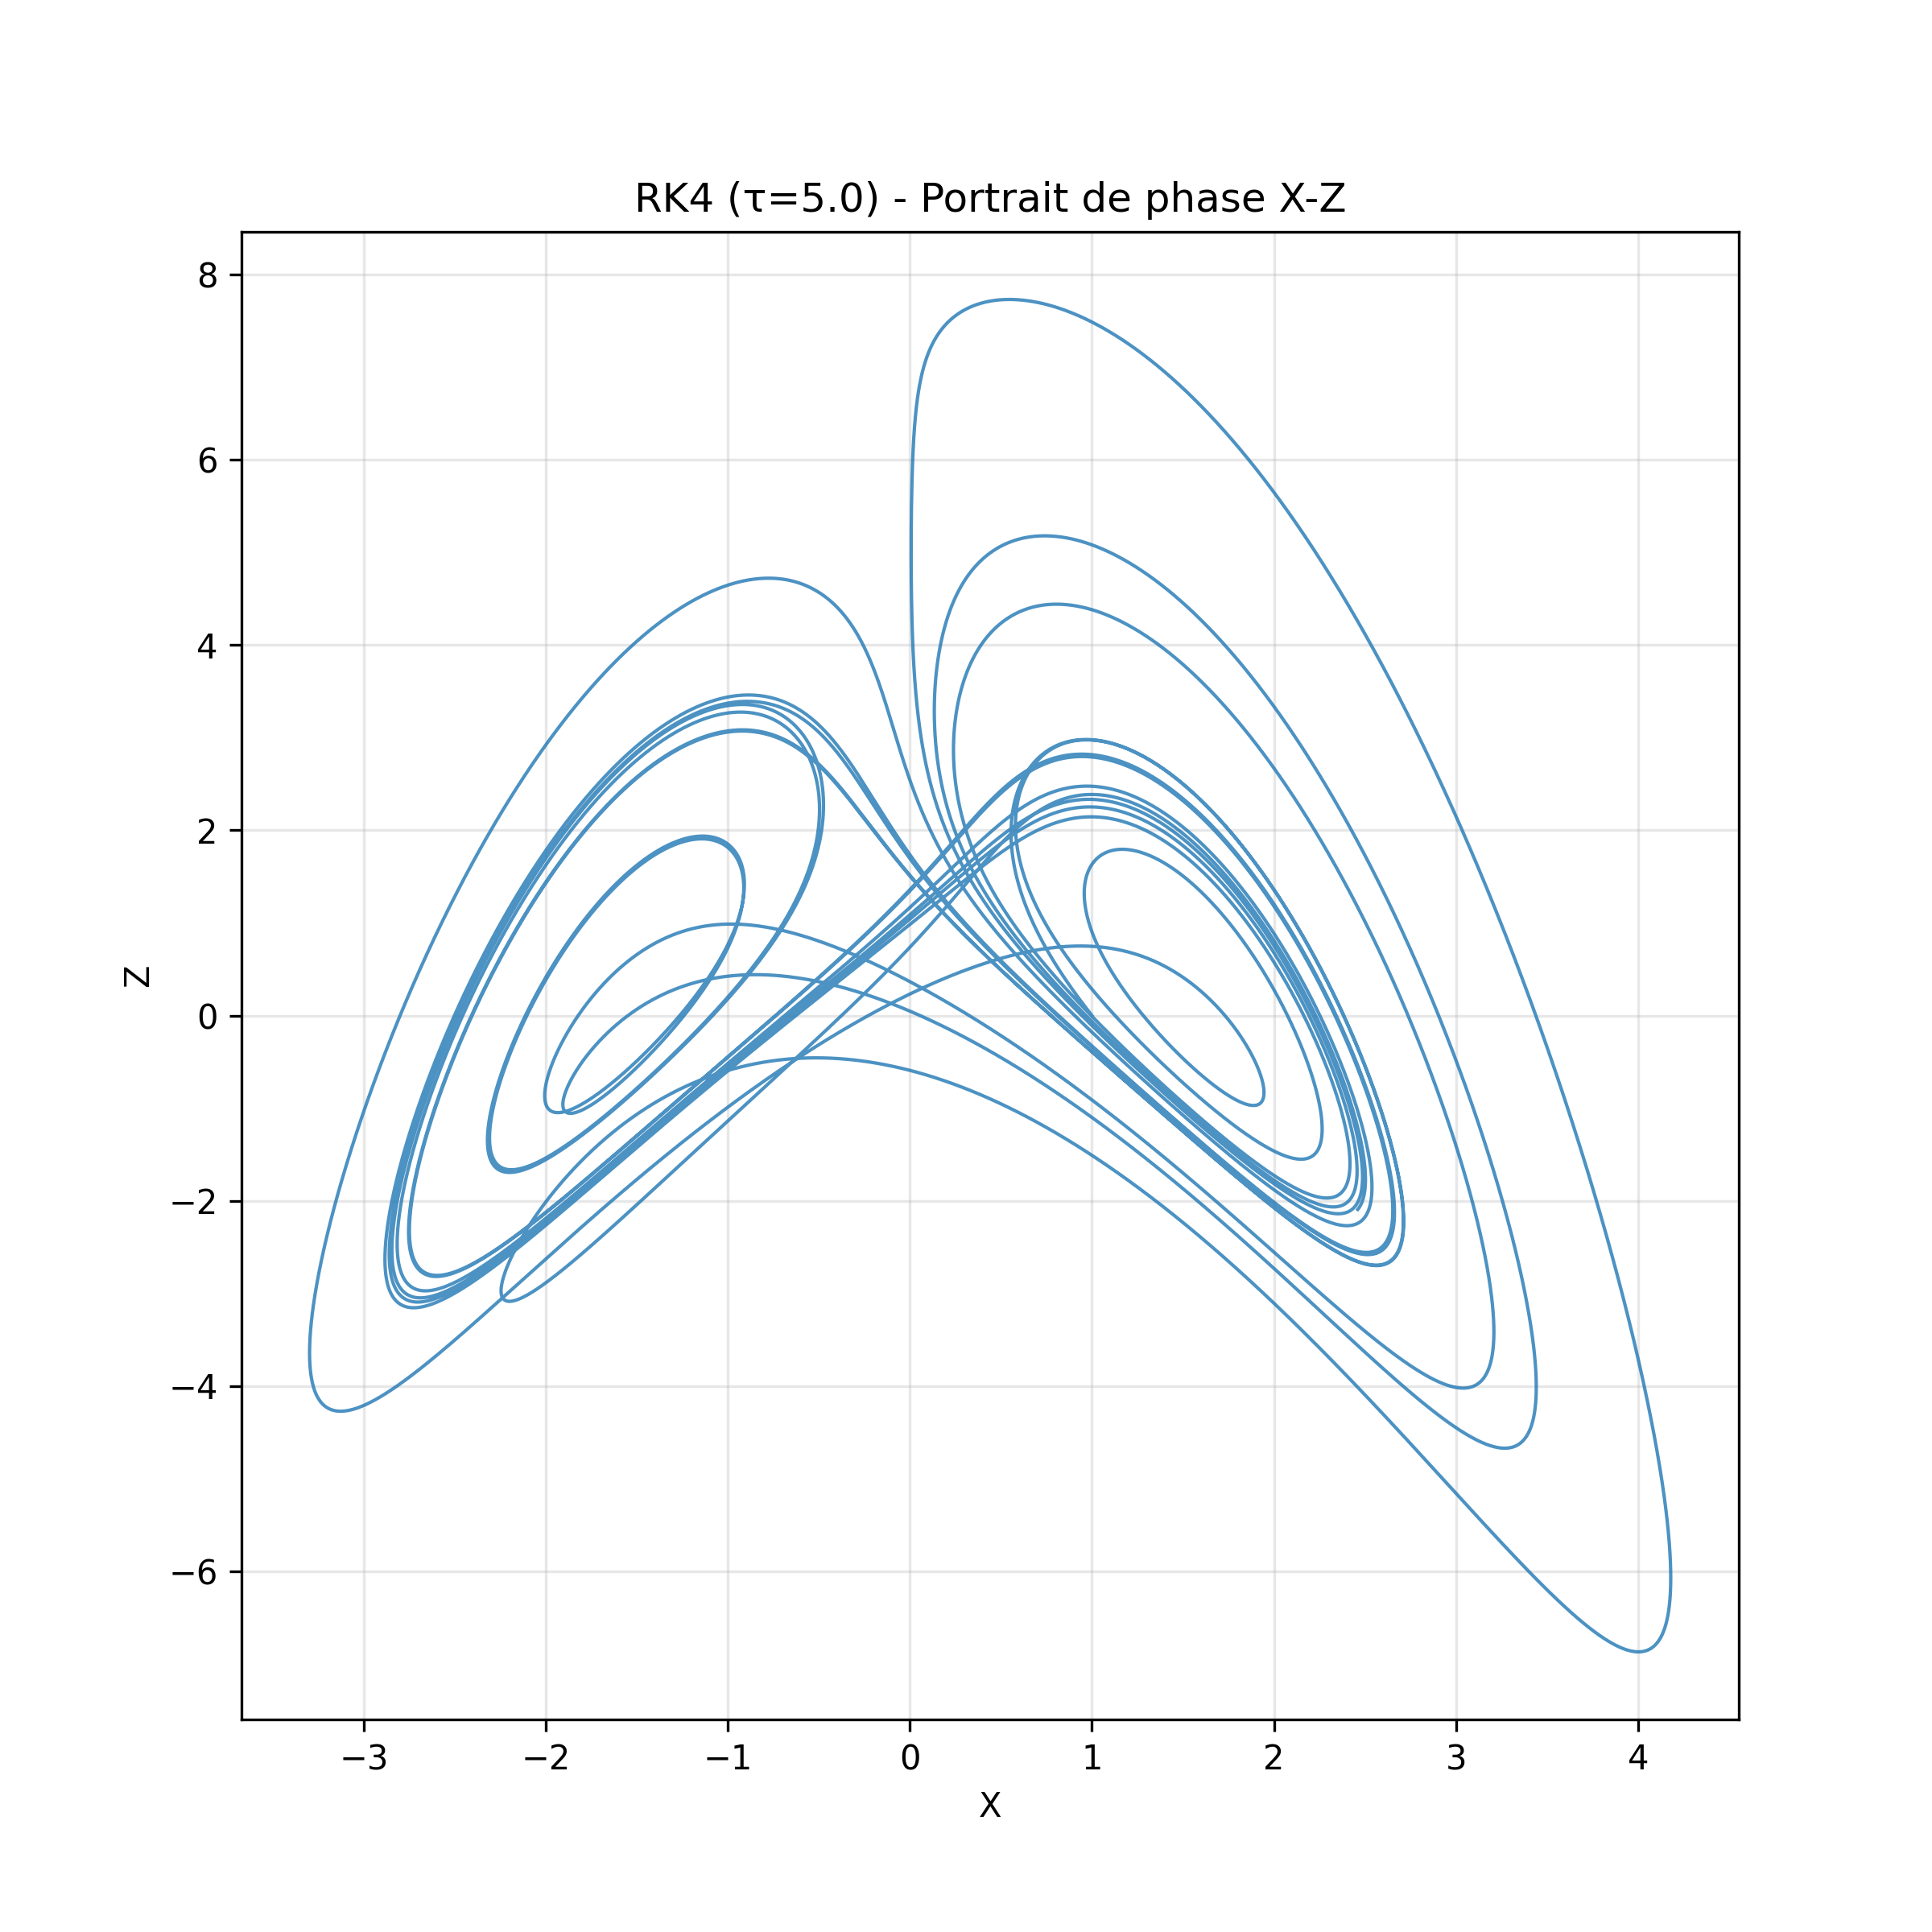
\includegraphics[width=\textwidth]{figures/rk4/rk4_tau5.0_phase}
        \caption{Portrait de phase : Attracteur étrange avec structure fractale complexe.}
    \end{subfigure}
    \caption{Dynamique pour $\tau$ = 5.0 : oscillations complexes}
    \label{fig:rk4_tau5.0}
\end{figure}

\subsubsection{Oscillations avec Dérive ($\tau$ = 8.9)}
Pour $\tau$ = 8.9, le système entre dans un régime pleinement chaotique.

Les oscillations sont quasi-périodiques avec une dérive progressive, et les motifs sont de plus en plus complexes. La structure est plus organisé que le scénario chaotique précédent, mais moins stable que le scénario de 
\begin{figure}[H]
    \centering
    \begin{subfigure}[b]{0.5\textwidth}
        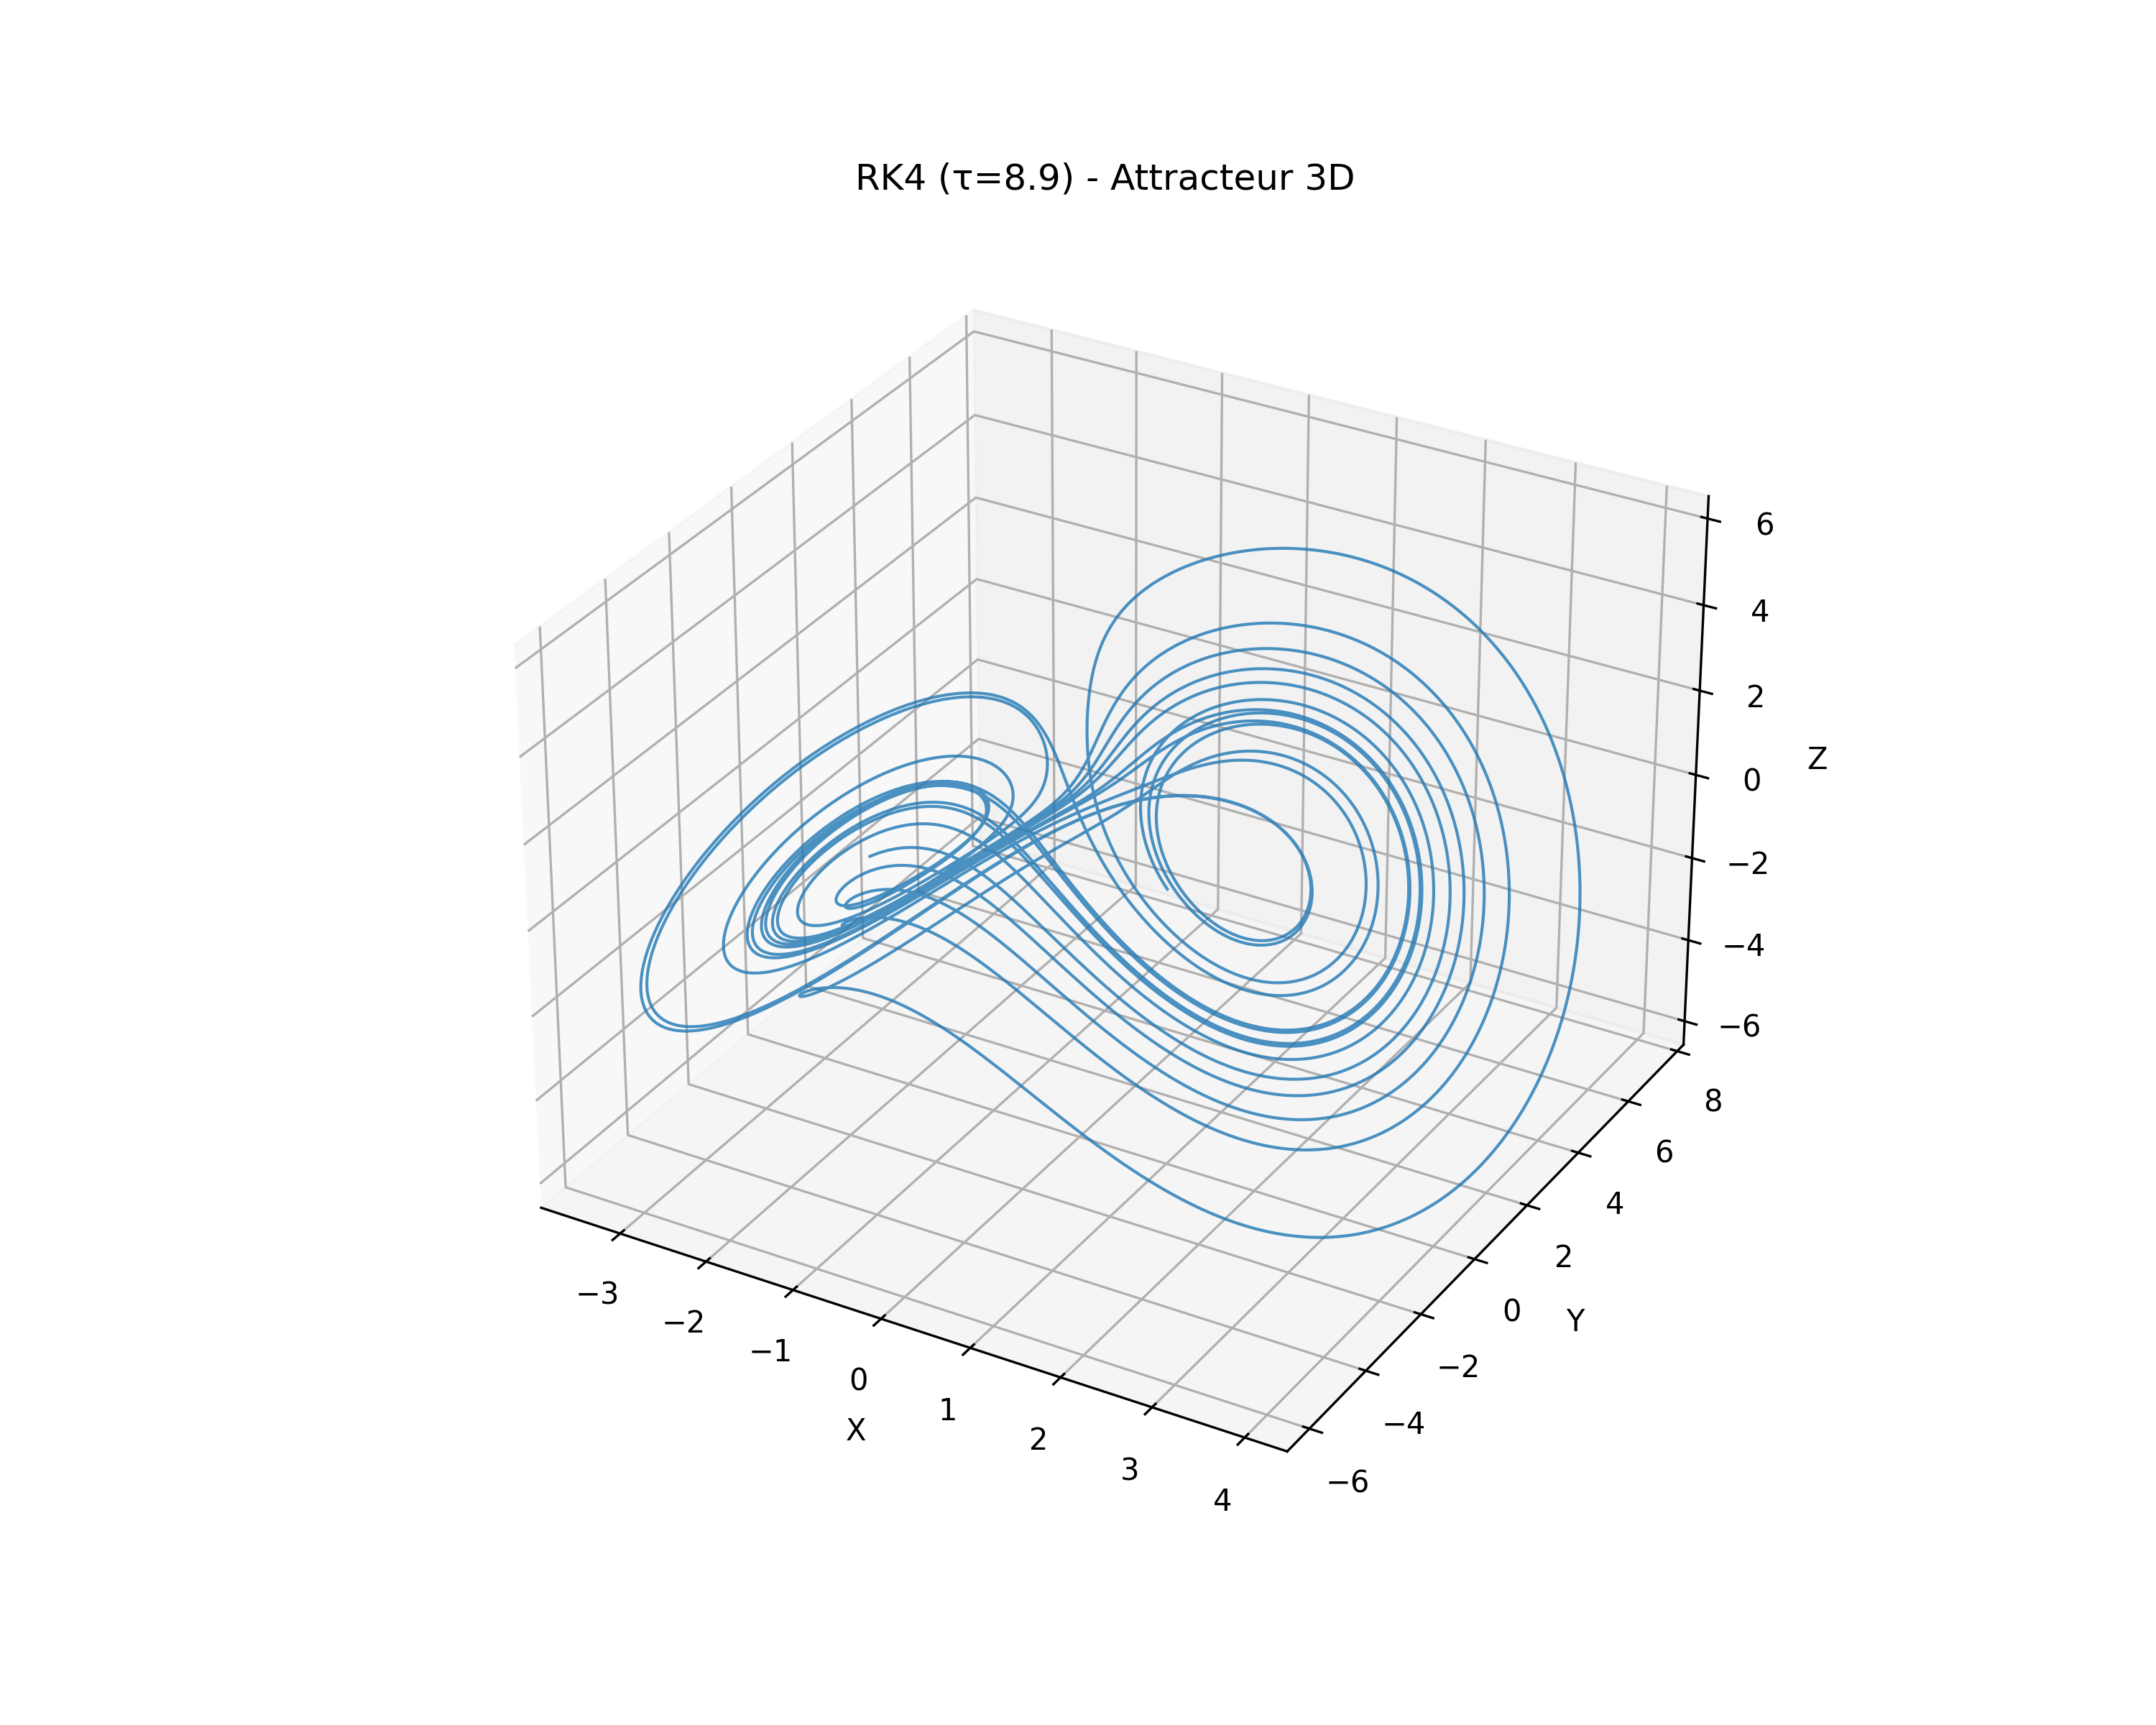
\includegraphics[width=\textwidth]{figures/rk4/rk4_tau8.9_3d}
        \caption{Trajectoire 3D : Structure intermédiaire entre l'attracteur chaotique et le point fixe}
    \end{subfigure}
    \begin{subfigure}[b]{0.4\textwidth}
        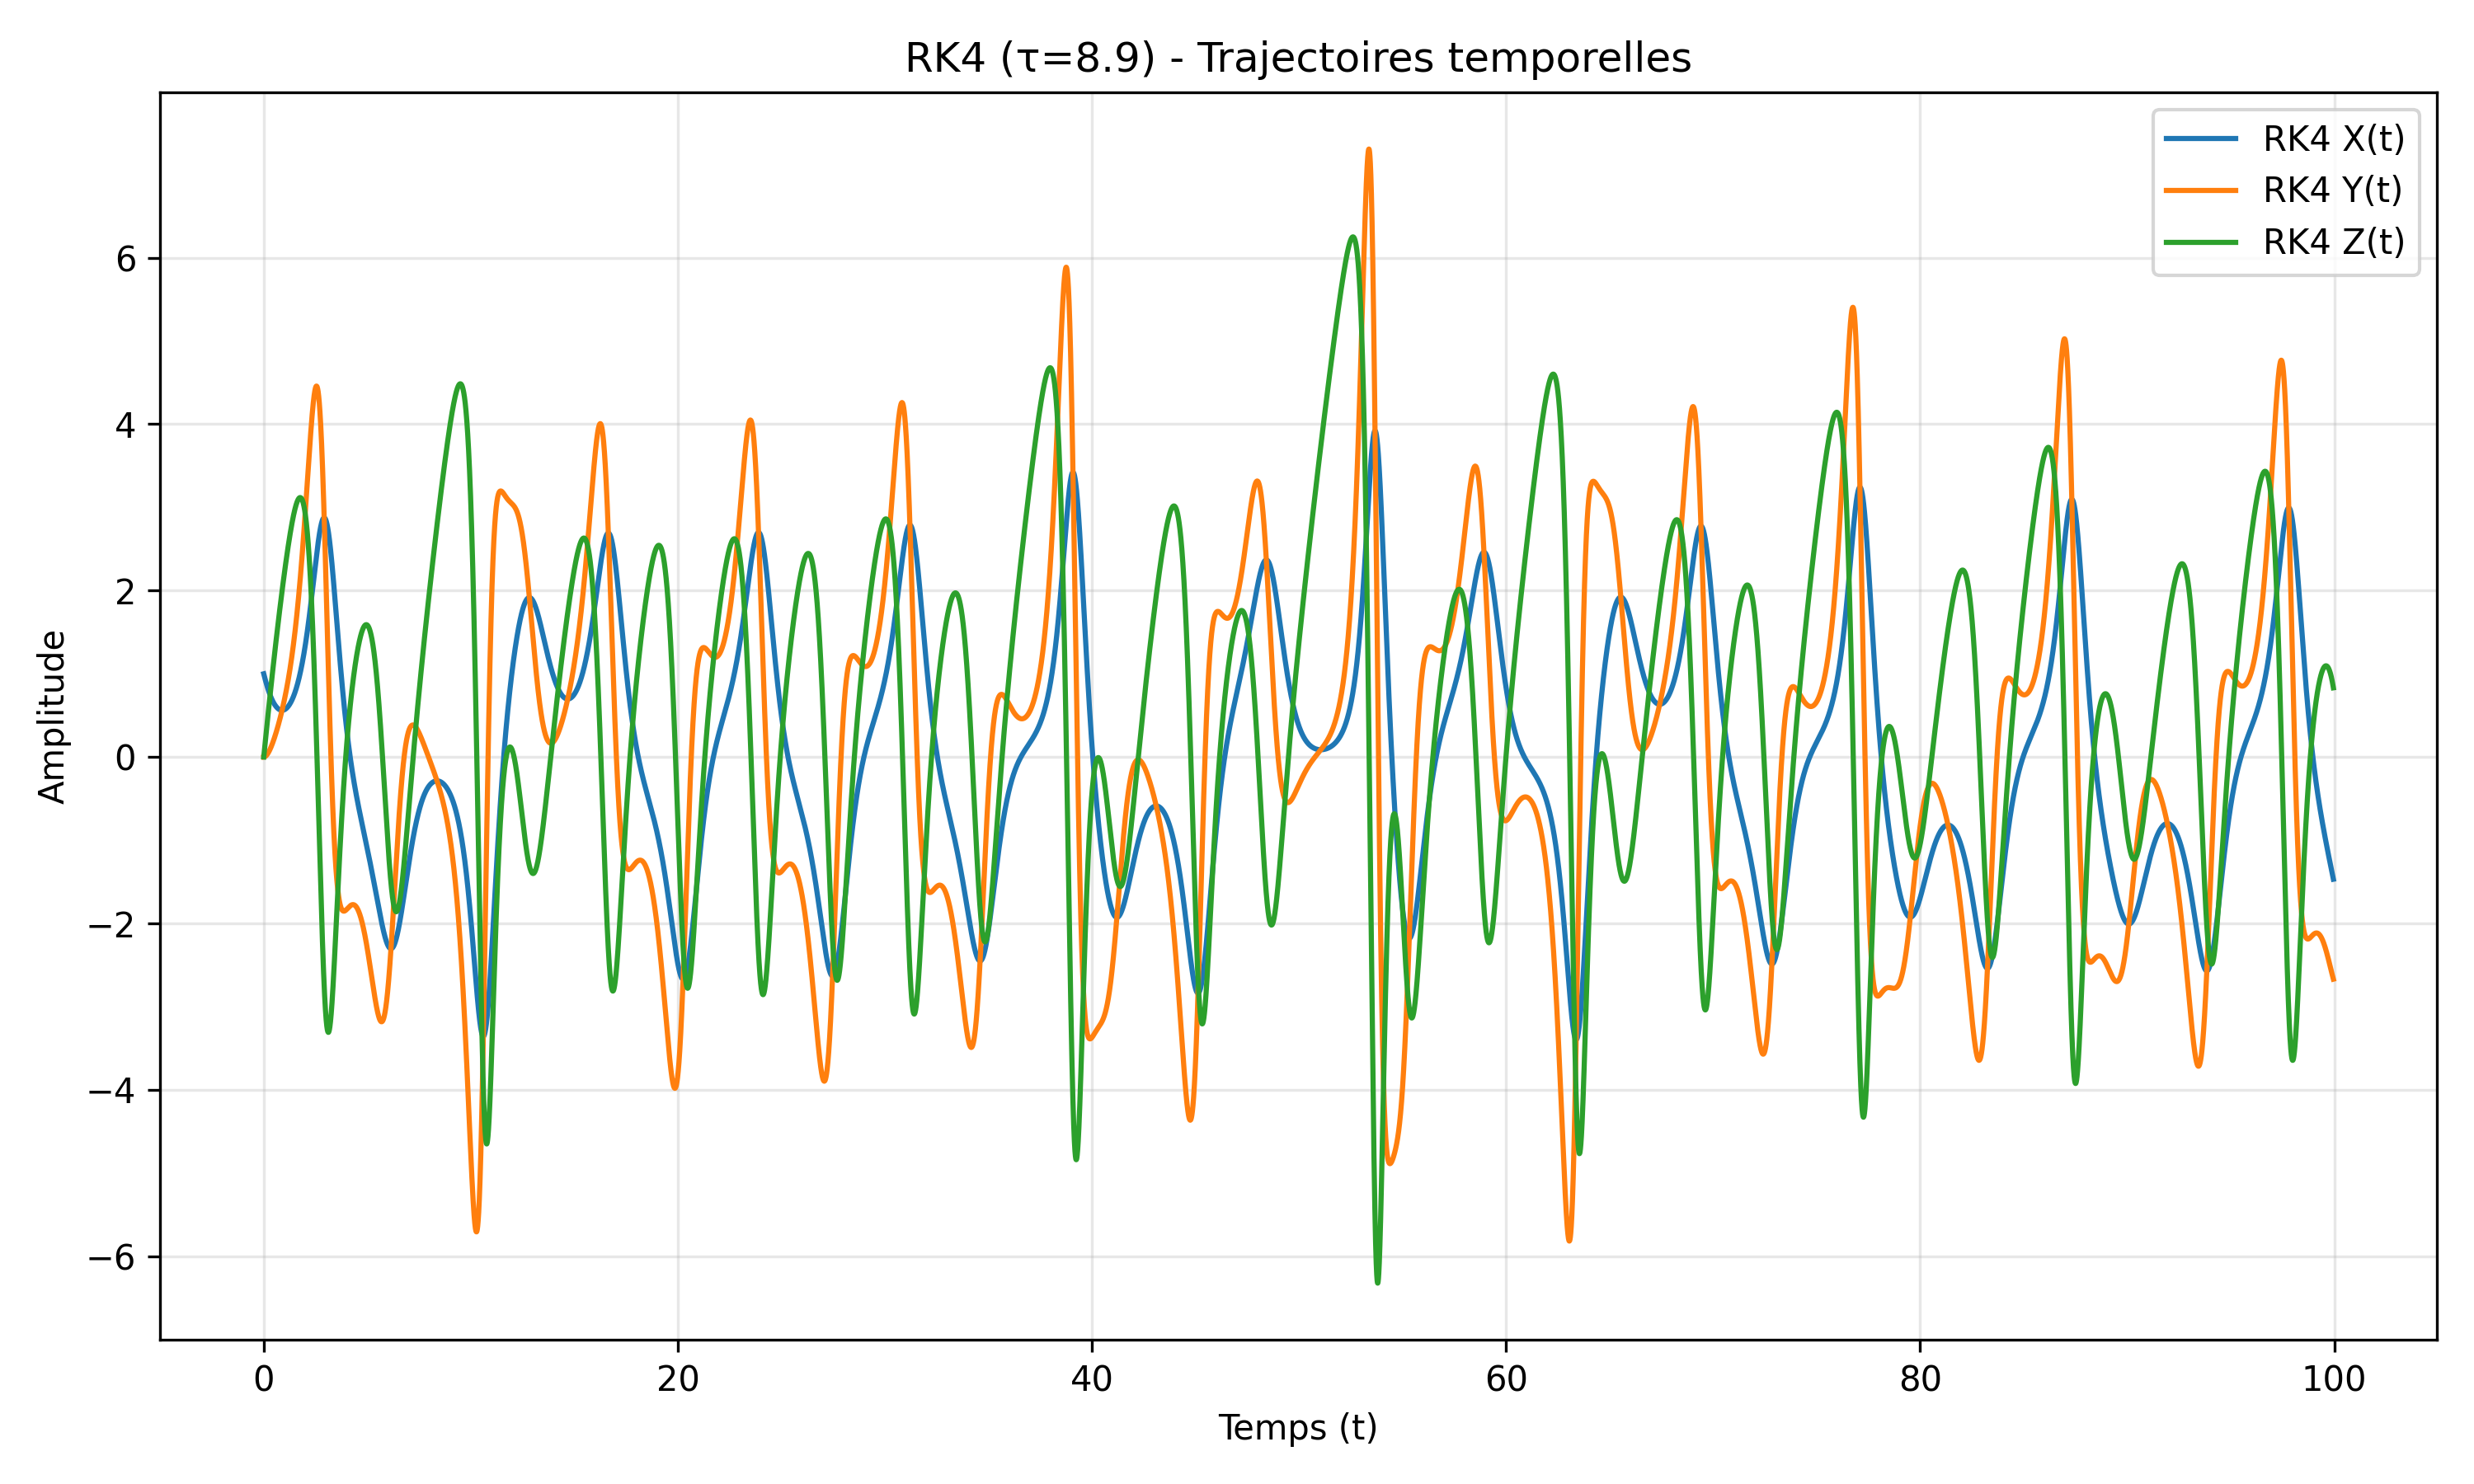
\includegraphics[width=\textwidth]{figures/rk4/rk4_tau8.9_time}
        \caption{Évolution temporelle : Oscillations avec une structure plus régulière mais avec dérive progressive}
    \end{subfigure}
    \begin{subfigure}[b]{0.3\textwidth}
        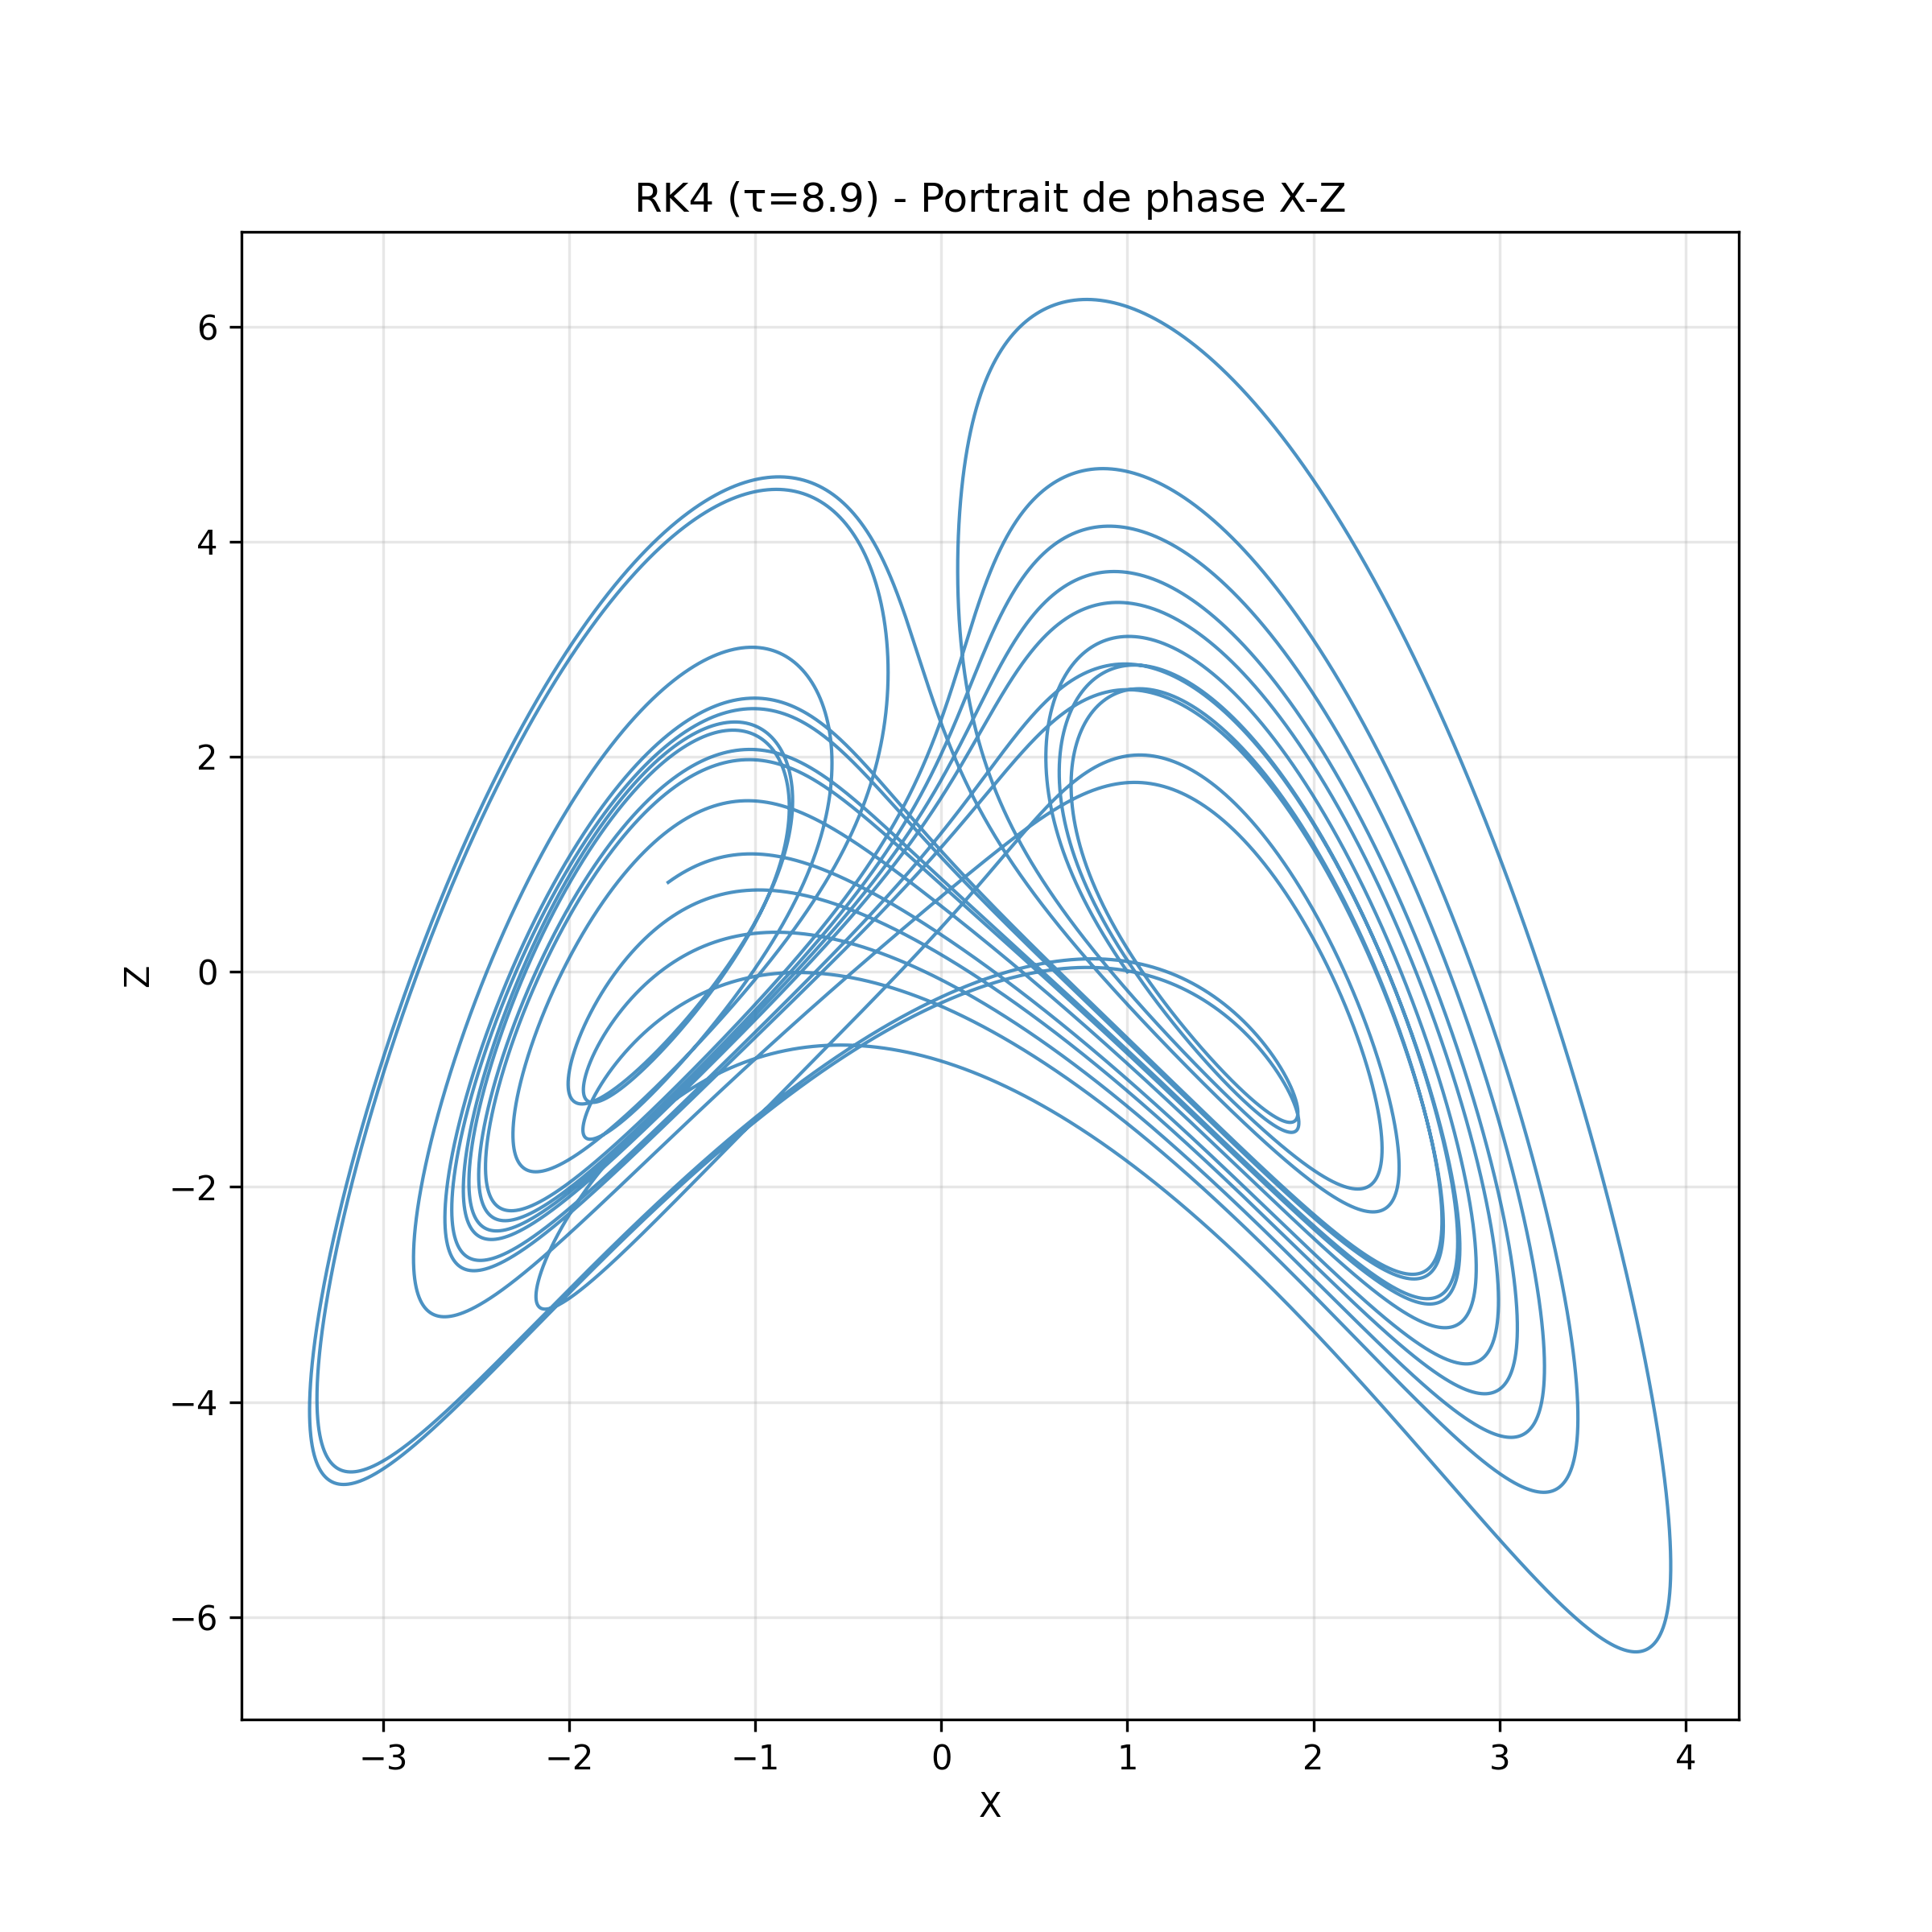
\includegraphics[width=\textwidth]{figures/rk4/rk4_tau8.9_phase}
        \caption{Portrait de phase : Trajectoire plus ordonnée mais non-périodique, formant un cycle limite déformé}
    \end{subfigure}
    \caption{Dynamique pour $\tau$ = 8.9 : comportement oscillatoire avec dérive}
    \label{fig:rk4_tau8.9}
\end{figure}

\subsection{Synthèse des résultats}
Les simulations numériques confirment parfaitement les comportements théoriques attendus pour chaque régime dynamique :

\begin{itemize}
    \item \textbf{État Non-Marcheur} ($\tau = 0.5$) : Convergence rapide vers l'origine, démontrant la stabilité du point fixe
    \item \textbf{Marche Régulière} ($\tau = 2.0$) : Établissement d'états stationnaires non nuls, caractéristiques du mouvement de marche
    \item \textbf{Marche Chaotique} ($\tau = 5.0$) : Comportement complexe avec attracteur étrange, typique du chaos
    \item \textbf{Oscillations avec Dérive} ($\tau = 8.9$) : Structure intermédiaire combinant oscillations et dérive progressive
\end{itemize}

\subsection{Limitations techniques}
La méthode RK4, bien que précise et stable, présente certaines limitations importantes :

\begin{enumerate}
    \item \textbf{Coût computationnel} : 4 évaluations de la fonction par pas de temps, rendant les simulations longues sur de grands intervalles
    \item \textbf{Stockage mémoire} : Nécessité de conserver les états intermédiaires, particulièrement problématique pour les systèmes de grande dimension
    \item \textbf{Parallélisation} : Impossible due à la dépendance séquentielle entre les pas de temps
\end{enumerate}

Ces limitations justifient l'exploration d'approches alternatives comme l'algorithme Parareal pour les simulations à grande échelle, particulièrement dans les régimes chaotiques où une haute précision est nécessaire.
\clearpage

% Algorithme Parareal
% Parareal Algorithm slides

\begin{frame}{Principe fondamental}
    \begin{itemize}
        \item Solution à la barrière de séquentialité temporelle
        \item \textbf{Éléments clés :}
        \begin{itemize}
            \item Décomposition du domaine temporel
            \item Deux niveaux de propagateurs
            \item Processus itératif de correction
        \end{itemize}
        \item \textbf{Avantages :}
        \begin{itemize}
            \item Calcul parallèle sur différents intervalles
            \item Maintien de la précision
            % \item Convergence garantie
        \end{itemize}
    \end{itemize}
\end{frame}

\begin{frame}{Architecture à deux niveaux}
    \begin{itemize}
        \item \textbf{Propagateur grossier $\mathcal{G}$}
        \begin{itemize}
            \item Rapide mais approximatif
            \item Basé sur RK2 ou méthode d'Euler
            \item Prédiction initiale
        \end{itemize}
        \vspace{0.3cm}
        \item \textbf{Propagateur fin $\mathcal{F}$}
        \begin{itemize}
            \item Précis mais coûteux
            \item Basé sur RK4
            \item Exécution parallèle
        \end{itemize}
    \end{itemize}
\end{frame}

\begin{frame}{Processus itératif}
    \begin{enumerate}
        \item \textbf{Initialisation}
        \begin{itemize}
            \item Division de $[0,T]$ en $N$ sous-intervalles
            \item $U_n^0 = u_0$ pour $n = 0$
            \item Prédiction grossière : $U_{n+1}^0 = \mathcal{G}(T_n, U_n^0, \Delta T)$
        \end{itemize}
        \vspace{0.2cm}
        \item \textbf{Calcul parallèle}
        \begin{itemize}
            \item Calcul fin : $\mathcal{F}(T_n, U_n^k, \Delta T)$
            \item Formule de correction :
            \begin{equation*}
                U_{n+1}^{k+1} = \mathcal{G}(T_n, U_n^{k+1}, \Delta T) + \mathcal{F}(T_n, U_n^k, \Delta T) - \mathcal{G}(T_n, U_n^k, \Delta T)
            \end{equation*}
        \end{itemize}
    \end{enumerate}
\end{frame}

\begin{frame}{Application au système de Lorenz}
    \begin{itemize}
        \item \textbf{Adaptation des propagateurs}
        \begin{itemize}
            \item Propagateur grossier : RK2 avec pas adaptatif
            \item $\Delta t_{\mathcal{G}} = \min(\alpha\tau, \Delta T)$
            \item Propagateur fin : RK4 avec pas fin
            \item $\Delta t_{\mathcal{F}} = \frac{\Delta t_{\mathcal{G}}}{m}$
        \end{itemize}
        \vspace{0.3cm}
        \item \textbf{Considérations particulières}
        \begin{itemize}
            \item Gestion des différents régimes dynamiques
            \item Adaptation aux échelles de temps du système
            \item Conservation des invariants physiques
        \end{itemize}
    \end{itemize}
\end{frame}

\begin{frame}{Stratégies de convergence}
    \begin{itemize}
        \item \textbf{Critères adaptatifs}
        \begin{equation*}
            \varepsilon_k = \max\left\{\frac{\|U_n^{k+1} - U_n^k\|}{\|U_n^k\|}, \frac{|E_k - E_{k-1}|}{|E_k|}\right\} < \text{tol}
        \end{equation*}
        \item \textbf{Optimisations}
        \begin{itemize}
            \item Prédiction améliorée avec extrapolation
            \item Stockage intelligent des états intermédiaires
            \item Équilibrage de charge dynamique
        \end{itemize}
    \end{itemize}
\end{frame}
\clearpage

% Implémentation
\section{Implémentation}

\subsection{Architecture logicielle}
L'implémentation suit une architecture modulaire avec une séparation claire des responsabilités, organisée en trois niveaux principaux.

\begin{figure}[h]
    \centering
    \begin{tikzpicture}[
        block/.style={rectangle,draw,fill=primaryblue!20,minimum width=2.5cm,minimum height=1cm},
        subblock/.style={rectangle,draw,fill=primaryblue!10,minimum width=2cm,minimum height=0.8cm},
        arrow/.style={->,thick},
        ]
        
        % Niveau 1 : Programme principal
        \node[block] (main) at (0,2) {Programme principal (main.f90)};
        
        % Niveau 2 : Modules principaux
        \node[block] (solvers) at (-4,0) {Solveurs};
        \node[block] (parareal) at (0,0) {Parareal};
        \node[block] (domain) at (4,0) {Décomposition};
        
        % Niveau 3 : Sous-modules
        \node[subblock] (rk4) at (-6,-2) {RK4};
        \node[subblock] (ab) at (-4,-2) {AB2/AB3};
        \node[subblock] (euler) at (-2,-2) {Euler};
        \node[subblock] (mpi) at (0,-2) {MPI};
        \node[subblock] (conv) at (2,-2) {Convergence};
        \node[subblock] (deriv) at (4,-2) {Dérivées};
        
        % Connexions niveau 1-2
        \draw[arrow] (main) -- (solvers);
        \draw[arrow] (main) -- (parareal);
        \draw[arrow] (main) -- (domain);
        
        % Connexions niveau 2-3
        \draw[arrow] (solvers) -- (rk4);
        \draw[arrow] (solvers) -- (ab);
        \draw[arrow] (solvers) -- (euler);
        \draw[arrow] (parareal) -- (mpi);
        \draw[arrow] (parareal) -- (conv);
        \draw[arrow] (domain) -- (deriv);
        
        % Connexions horizontales
        \draw[arrow, dashed] (rk4) -- (mpi);
        \draw[arrow, dashed] (ab) -- (mpi);
        \draw[arrow, dashed] (euler) -- (mpi);
    \end{tikzpicture}
    \caption{Architecture détaillée du système}
    \label{fig:architecture_detailed}
\end{figure}

\begin{figure}[H]
    \centering
    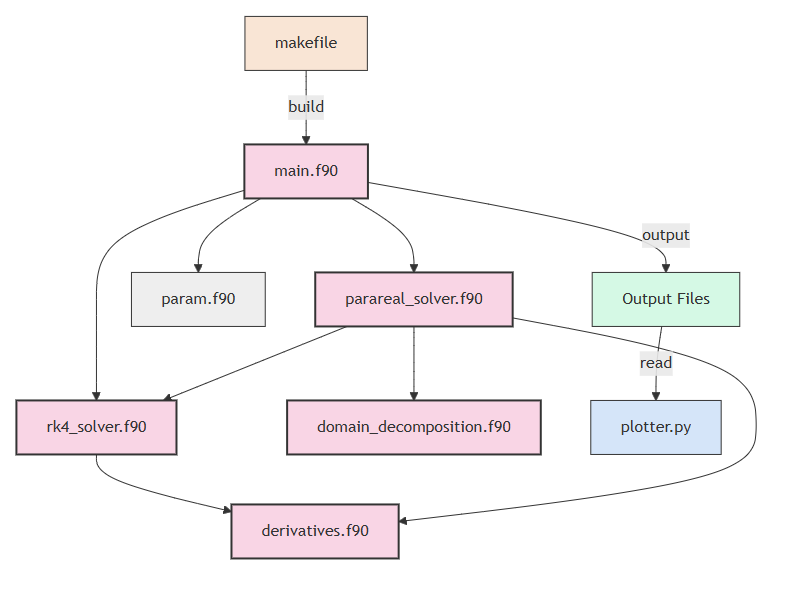
\includegraphics[width=0.8\textwidth]{code/figure.png}
    \caption{Architecture logicielle : modules et sous-modules}
    \label{fig:architecture}
\end{figure}

\subsection{Composants principaux}

\subsubsection{Programme principal (main.f90)}
Point d'entrée centralisant :
\begin{itemize}
    \item Gestion des arguments et configurations
    \item Initialisation MPI et distribution des tâches
    \item Coordination des solveurs et mesure des performances
\end{itemize}

\subsubsection{Module de solveurs}
Implémente trois niveaux de solveurs :

\begin{enumerate}
    \item \textbf{Solveur fin (RK4)} :
    \begin{itemize}
        \item Haute précision pour les calculs critiques
        \item Adaptation automatique du pas de temps
        \item Détection et gestion des instabilités
    \end{itemize}

    \item \textbf{Solveurs intermédiaires (AB2/AB3)} :
    \begin{itemize}
        \item Compromis précision/performance
        \item Stabilisation par amortissement
        \item Mélange avec l'historique pour les régimes chaotiques
    \end{itemize}

    \item \textbf{Solveur grossier (Euler)} :
    \begin{itemize}
        \item Rapidité d'exécution pour les prédictions initiales
        \item Robustesse pour les grands pas de temps
        \item Adaptation aux différents régimes de $\tau$
    \end{itemize}
\end{enumerate}

\subsection{Mécanismes de stabilité et sécurité}

\subsubsection{Adaptation aux régimes dynamiques}
Le système ajuste automatiquement ses paramètres selon la valeur de $\tau$ :

\begin{lstlisting}[language=Fortran,caption=Adaptation dynamique des paramètres]
if (tau < 1.0) then  ! Régime non-marcheur
    h_coarse = min(h_coarse, tau/20.0)
    h_fine = min(h_fine, tau/200.0)
    adapt_tol = min(tol, 1.0E-5)
else if (tau < 3.0) then  ! Marche régulière
    h_coarse = min(h_coarse, tau/10.0)
    h_fine = min(h_fine, tau/100.0)
    adapt_tol = min(tol, 5.0E-6)
else  ! Régimes chaotiques
    h_coarse = min(h_coarse, 0.1)
    h_fine = min(h_fine, 0.01)
    adapt_tol = min(tol, 1.0E-6)
end if
\end{lstlisting}

\subsubsection{Mécanismes de protection}
Implémentation de plusieurs niveaux de sécurité :

\begin{lstlisting}[language=Fortran,caption=Circuit breaker pour les instabilités]
if (any(isnan(u)) .or. any(abs(u) > MAX_VALUE)) then
    bad_value_counter = bad_value_counter + 1
    where (isnan(u)) u = 0.0
    where (abs(u) > MAX_VALUE) 
        u = sign(MAX_VALUE, u)
    end where
    
    if (bad_value_counter >= MAX_BAD_ITER) then
        status = ERROR_UNSTABLE
        return
    end if
end if
\end{lstlisting}

\subsection{Parallélisation avancée}
\subsubsection{Distribution et équilibrage}
La décomposition temporelle utilise une stratégie adaptative :

\begin{lstlisting}[language=Fortran,caption=Distribution des intervalles]
subroutine distribute_intervals(total_intervals, size, rank, 
                              start_idx, end_idx)
    integer, intent(in) :: total_intervals, size, rank
    integer, intent(out) :: start_idx, end_idx
    integer :: base_count, remainder
    
    base_count = total_intervals / size
    remainder = mod(total_intervals, size)
    
    if (rank < remainder) then
        start_idx = rank * (base_count + 1) + 1
        end_idx = start_idx + base_count
    else
        start_idx = rank * base_count + remainder + 1
        end_idx = start_idx + base_count - 1
    end if
end subroutine distribute_intervals
\end{lstlisting}

\subsection{Visualisation et analyse}
Le système inclut des capacités avancées de visualisation :

\begin{itemize}
    \item Génération de trajectoires denses adaptées au régime :
    \begin{itemize}
        \item 50 points/intervalle pour $\tau$ < 2.0
        \item 75 points/intervalle pour 2.0 $\leq$ $\tau$ < 5.0
        \item 100 points/intervalle pour $\tau$ $\geq$ 5.0
    \end{itemize}
    \item Sauvegarde structurée des résultats pour post-traitement
    \item Scripts d'analyse automatisés pour validation
\end{itemize}

\subsection{Stratégies de convergence avancées}
L'algorithme implémente plusieurs stratégies sophistiquées pour assurer et accélérer la convergence :

\subsubsection{Critère de convergence adaptatif}
Le système utilise une métrique composite pour évaluer la convergence :

\begin{lstlisting}[language=Fortran,caption=Critère de convergence hybride]
! Changement d'état relatif
rel_state_change = max_diff / (maxval(abs(U_n)) + 1.0E-10)

! Conservation de l'énergie
rel_energy_change = abs(energy_k - energy_k_prev) 
                   / (abs(energy_k_prev) + 1.0E-10)

! Métrique combinée
conv_metric = max(rel_state_change, rel_energy_change)
converged = conv_metric < adapt_tol
\end{lstlisting}

\subsubsection{Prédiction améliorée}
Pour les régimes difficiles, une stratégie d'extrapolation est utilisée :

\begin{lstlisting}[language=Fortran,caption=Extrapolation pour prédiction]
if (k > 1) then
    ! Utilisation de l'historique des corrections
    U_new = propagate_with_ab3(...) + 
            beta * (U_n - U_prev)
    
    ! Stabilisation pour les petits tau
    if (tau < 1.0) then
        U_new = 0.8 * u_coarse_new + 
                0.2 * (u_fine - u_coarse_prev + u_coarse_new)
    end if
end if
\end{lstlisting}


L'ensemble du code implémenté est disponible en accès libre sur le dépôt GitHub suivant : https://github.com/KyFaxTeam/Parareal-Lorenz. 

\clearpage

% Résultats
\section{Résultats et analyse comparative}

\subsection{Méthodologie de comparaison}
Pour valider l'implémentation de l'algorithme Parareal et évaluer sa précision, nous avons effectué une comparaison systématique avec la méthode RK4 séquentielle. Pour chaque régime dynamique (caractérisé par différentes valeurs de $\tau$), nous avons analysé :
\begin{itemize}
    \item L'évolution temporelle des trois variables (X, Y, Z)
    \item L'erreur absolue entre les solutions Parareal et RK4 pour chacune des variables.
    \item La convergence vers l'état stationnaire ou l'attracteur chaotique
    \item Les portraits de phase dans les plans X-Z, Y-Z et X-Y
\end{itemize}

\subsection{Analyse par régime dynamique}

\subsubsection{Régime non-marcheur ($\tau$ = 0.5)}
Pour le régime de faible mémoire, où le système converge vers un point fixe :

\begin{figure}[H]
    \centering
    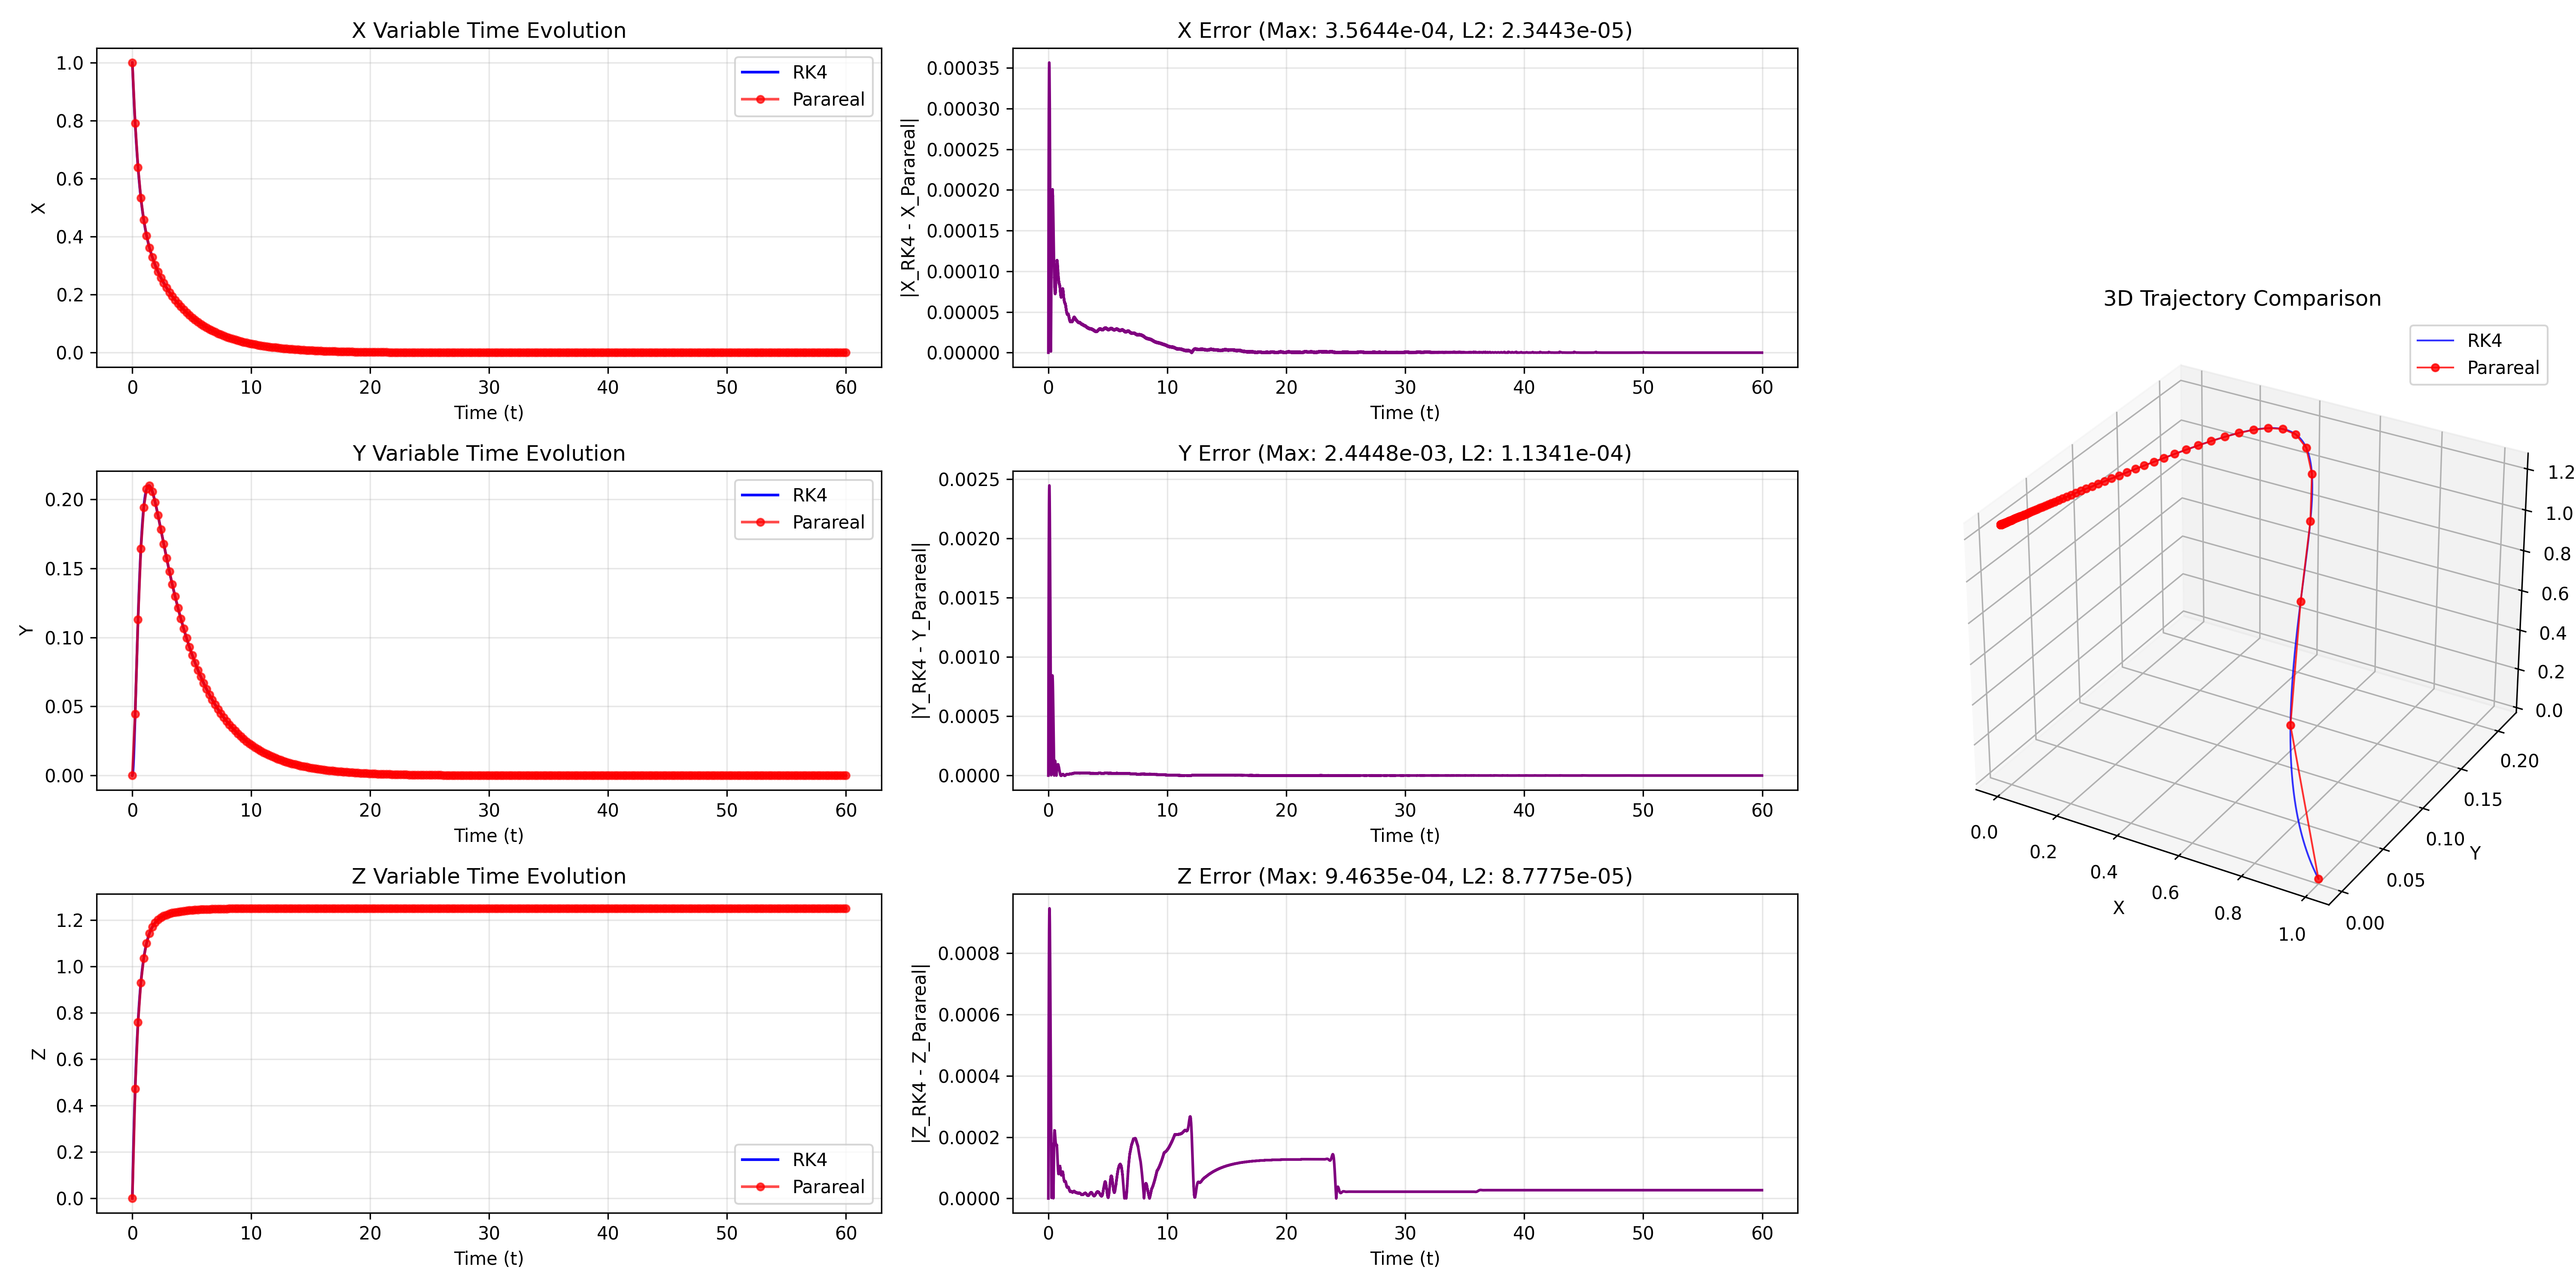
\includegraphics[width=\textwidth]{figures/comparisons/comparison_tau0.5_comparison}
    \caption{Comparaison des évolutions temporelles et erreurs temporelles pour $\tau$ = 0.5}
    \label{fig:comp_tau0.5_time}
\end{figure}

Les résultats montrent :
\begin{itemize}
    \item Une excellente concordance entre les deux méthodes dans la prédiction de la convergence vers l'origine
    \item Des erreurs absolues très faibles ($< 10^{-6}$) après la phase transitoire initiale
    \item Une stabilité numérique comparable pour les deux approches
\end{itemize}

\begin{figure}[H]
    \centering
    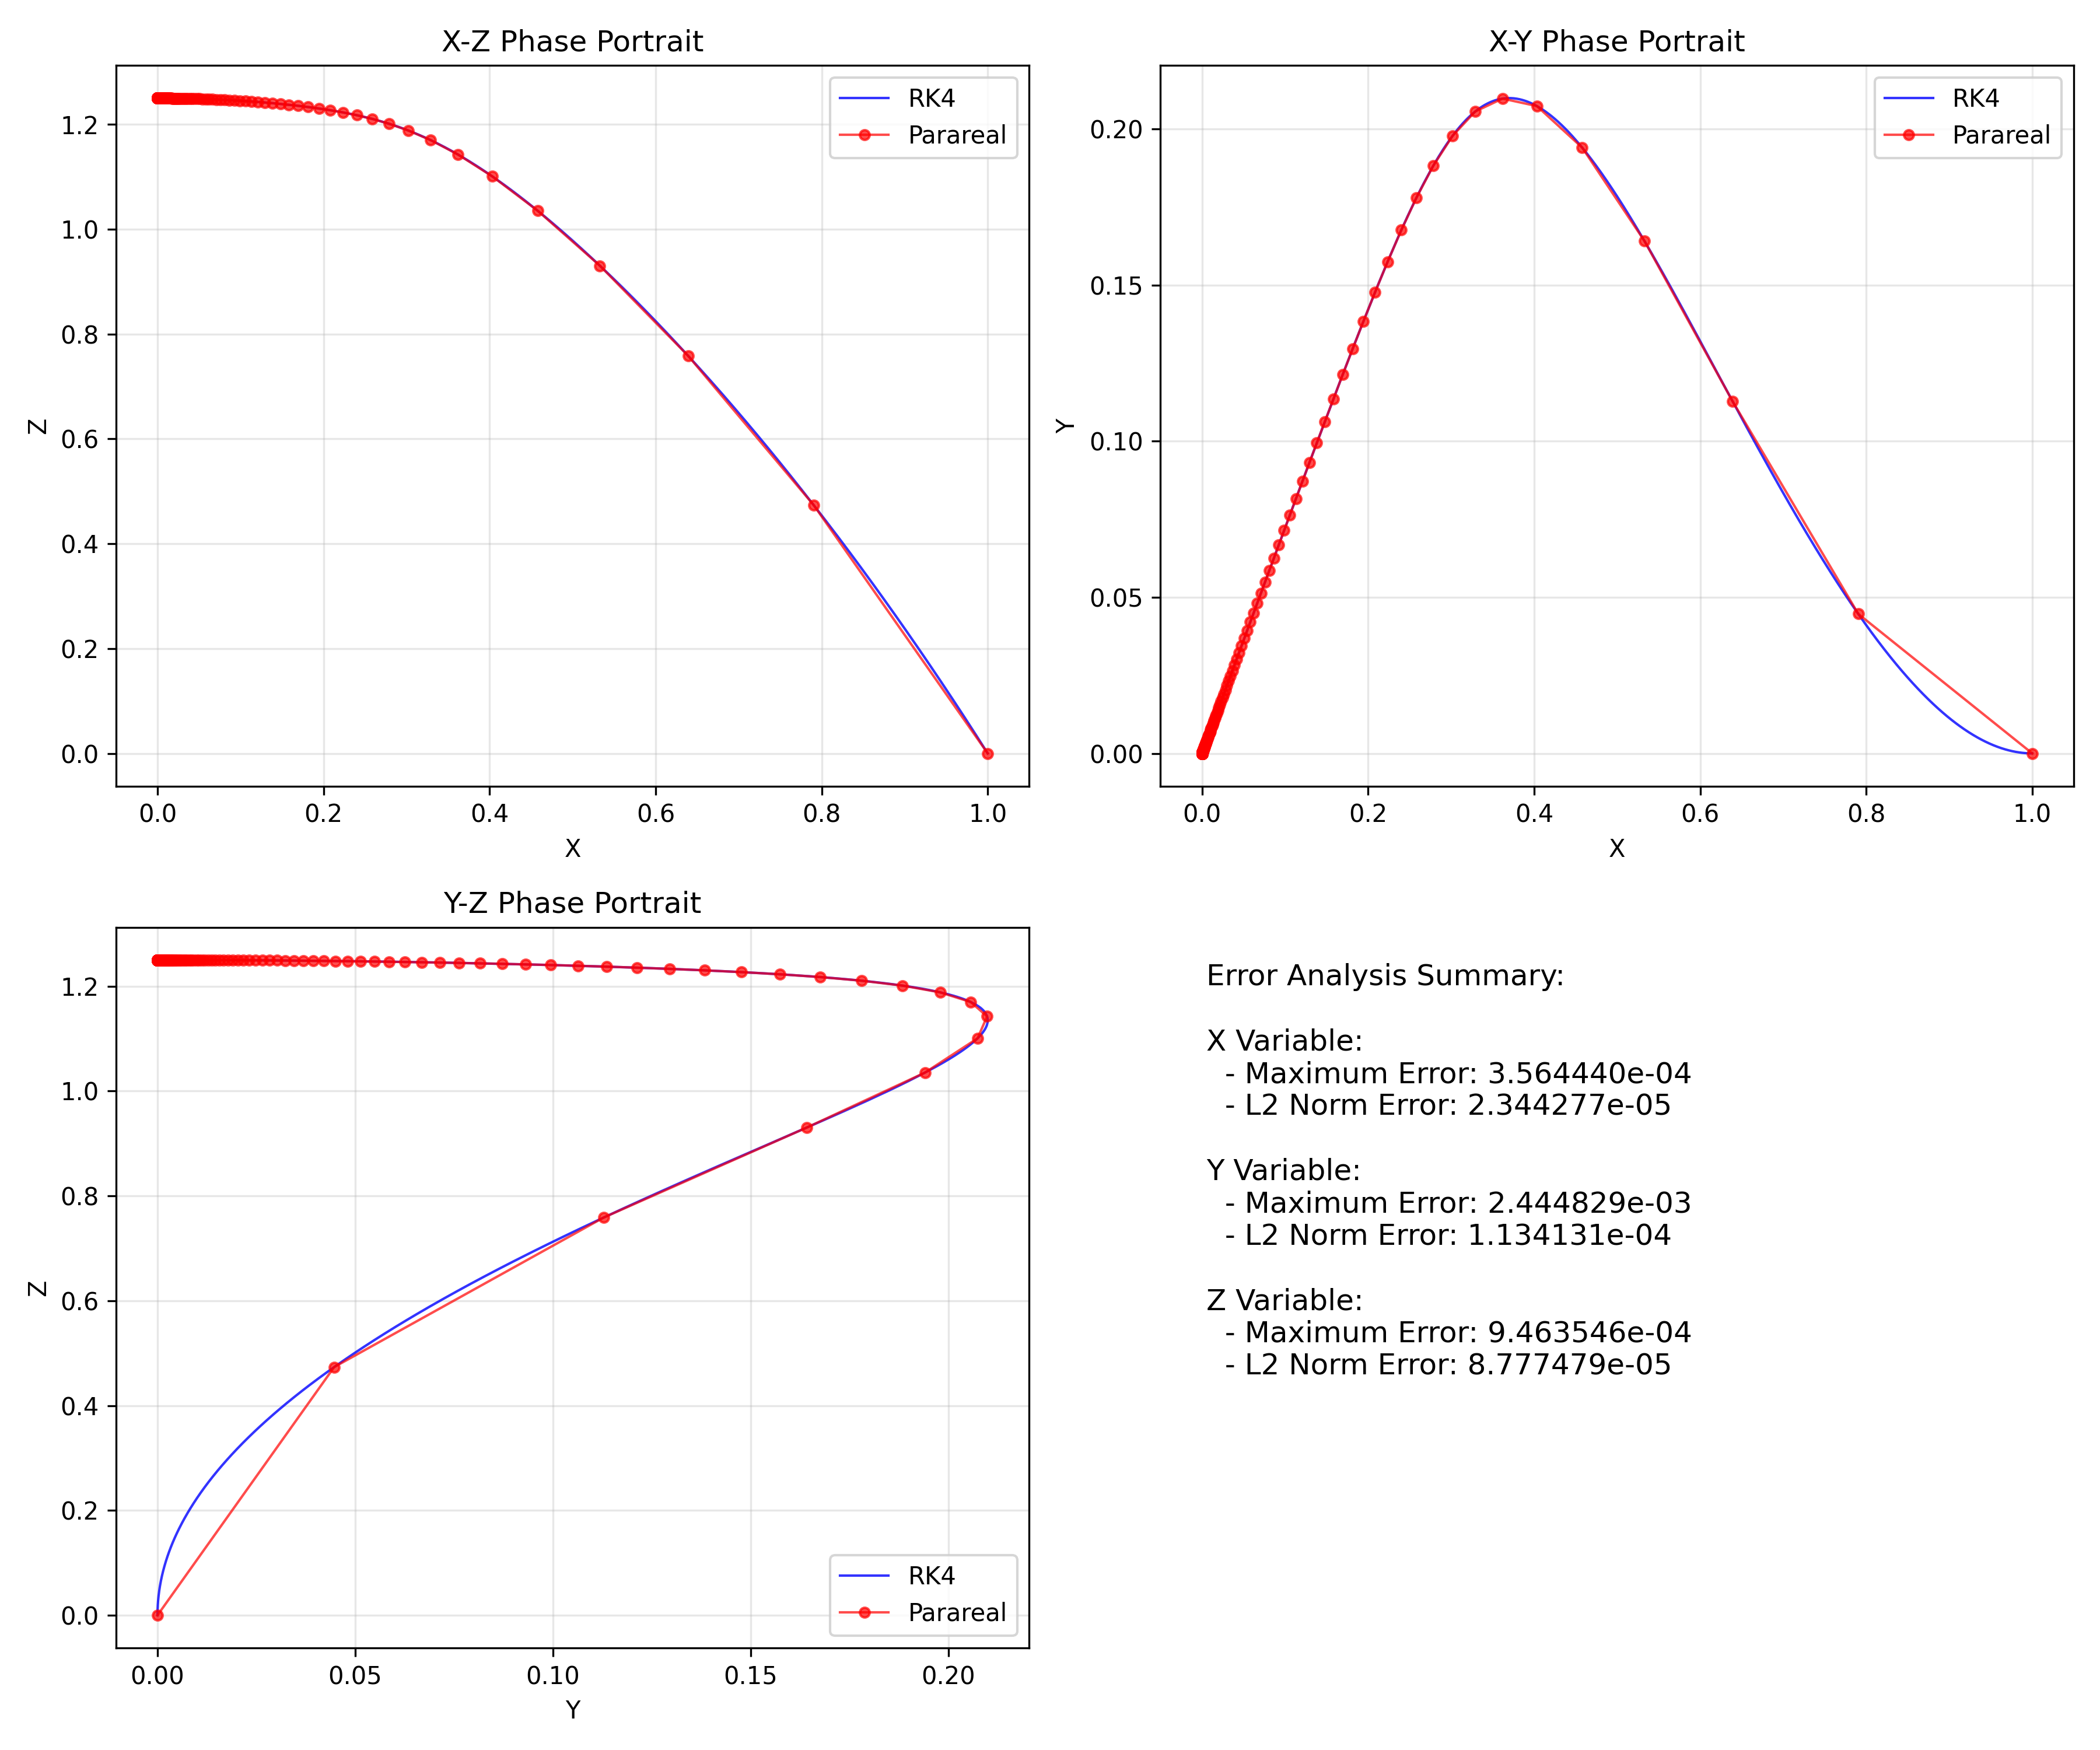
\includegraphics[width=\textwidth]{figures/comparisons/comparison_tau0.5_phase_portraits}
    \caption{Portraits de phase comparés pour $\tau$ = 0.5}
    \label{fig:comp_tau0.5_phase}
\end{figure}

Les portraits de phase confirment la précision de l'algorithme Parareal dans la capture de la dynamique de convergence.

\subsubsection{Régime de marche régulière ($\tau$ = 2.0)}
Pour le régime de marche stable :

\begin{figure}[H]
    \centering
    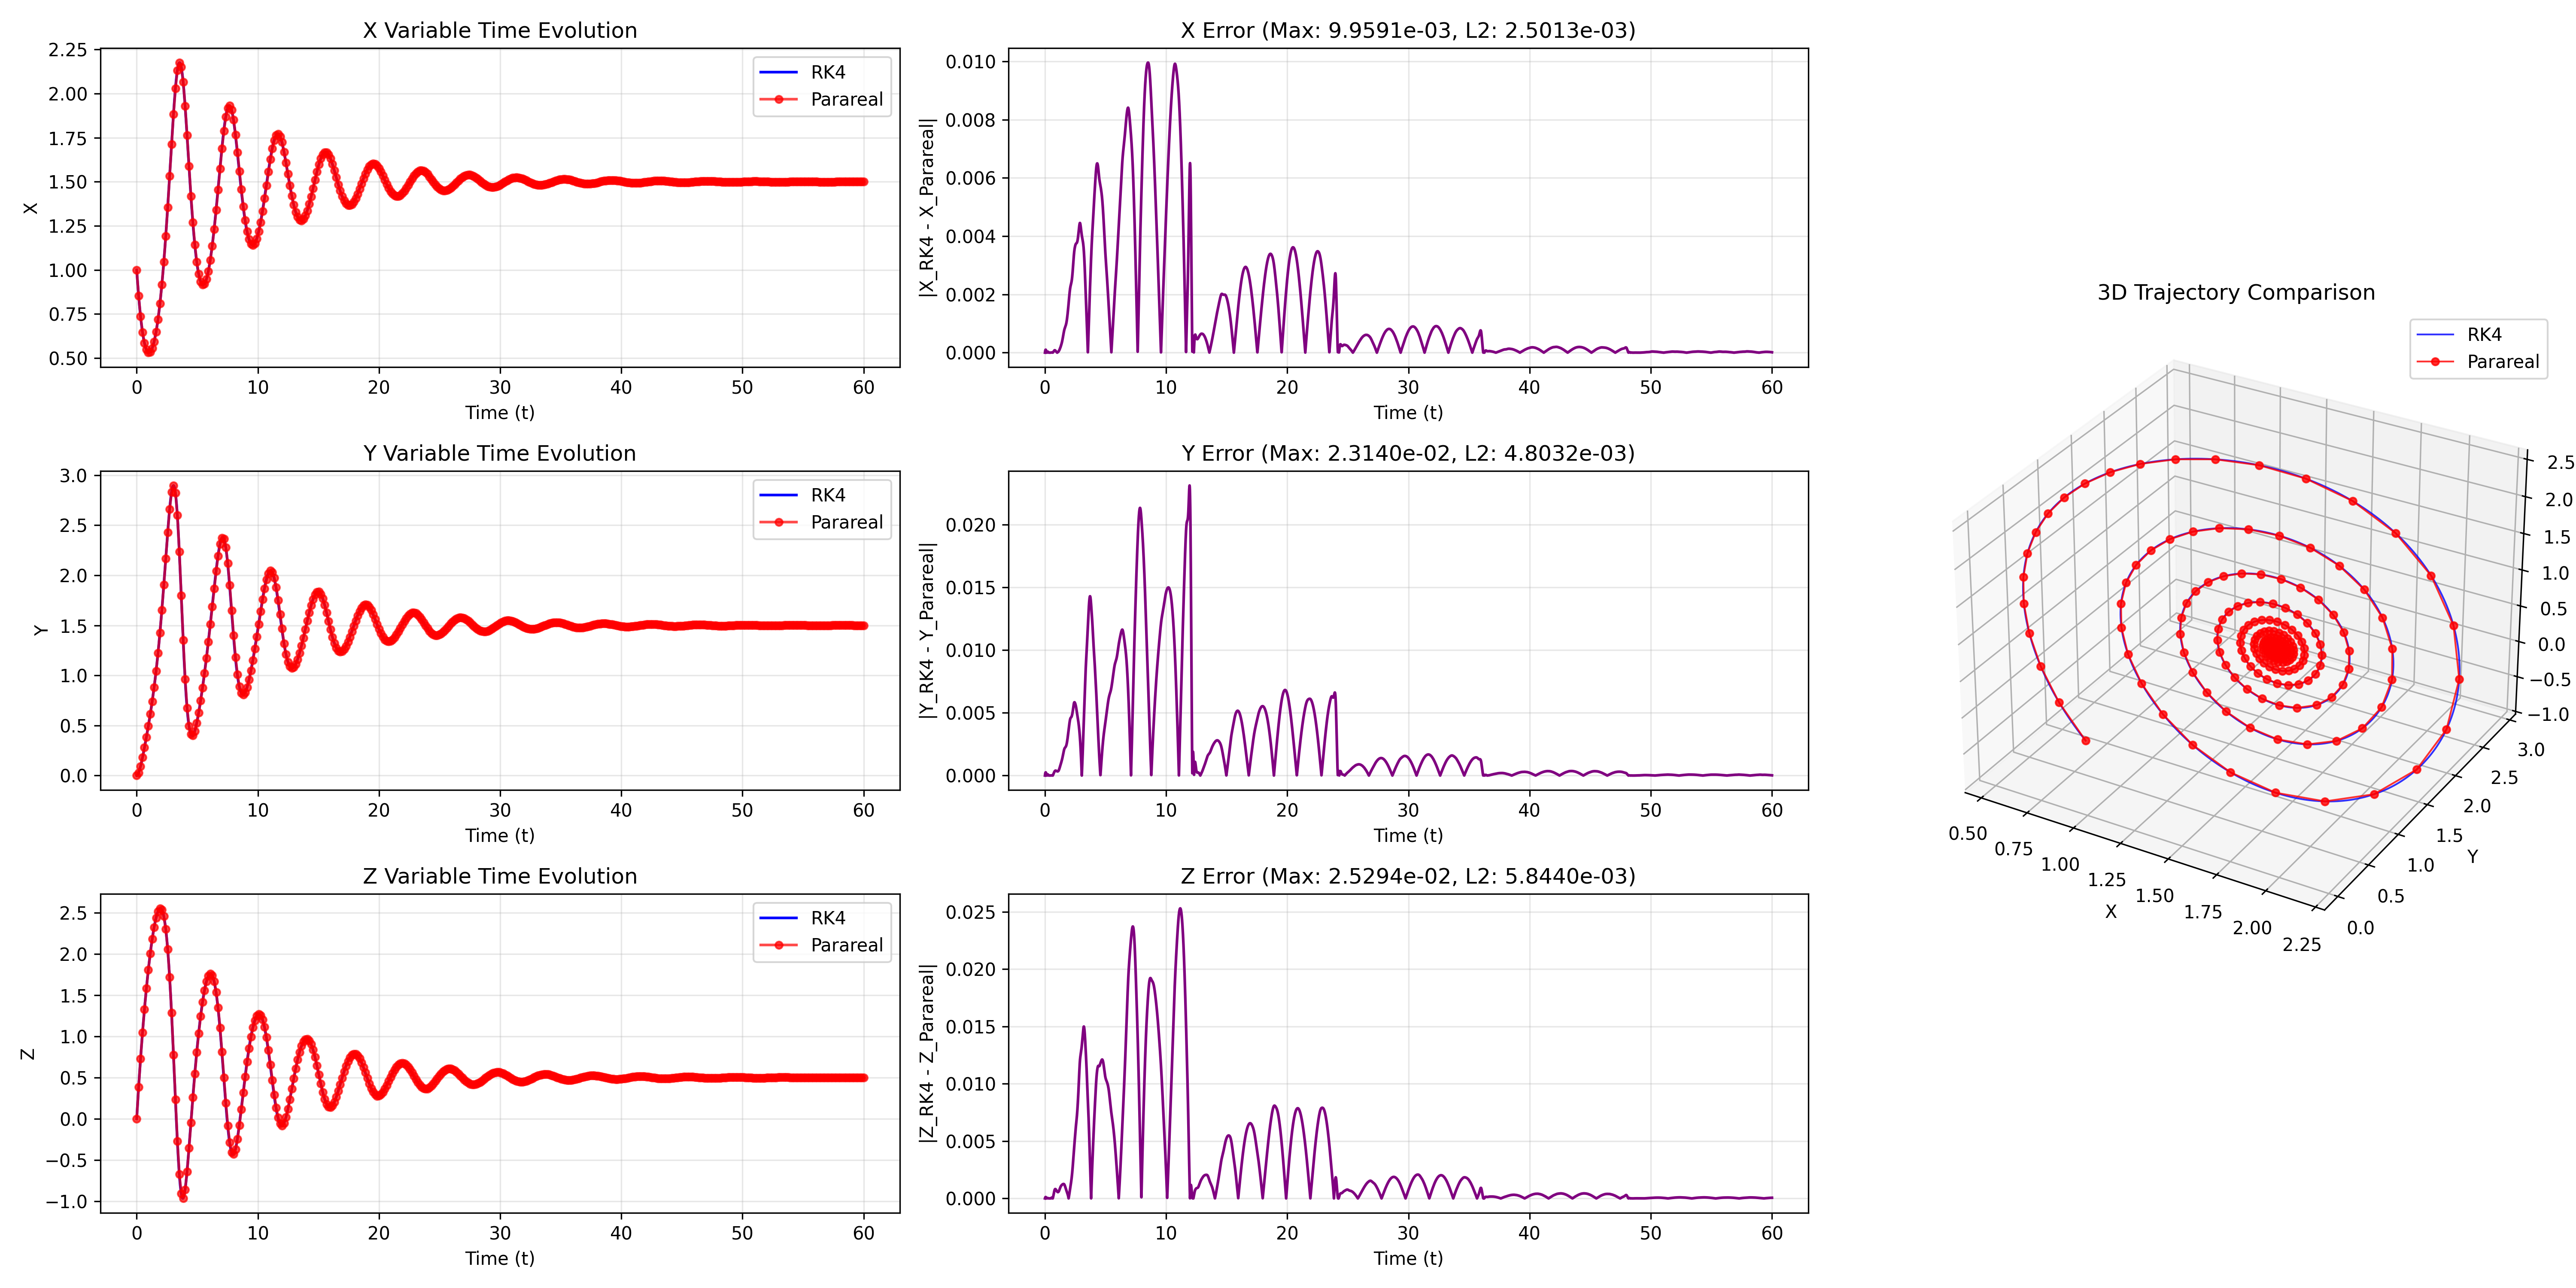
\includegraphics[width=\textwidth]{figures/comparisons/comparison_tau2.0_comparison}
    \caption{Comparaison des évolutions temporelles et erreurs absolues pour $\tau$ = 2.0}
    \label{fig:comp_tau2.0_time}
\end{figure}

L'analyse révèle :
\begin{itemize}
    \item Une reproduction fidèle des états stationnaires non-triviaux
    \item Une stabilisation rapide des erreurs à des niveaux très bas
    \item Une capacité à maintenir la précision sur de longues durées de simulation
\end{itemize}

\begin{figure}[H]
    \centering
    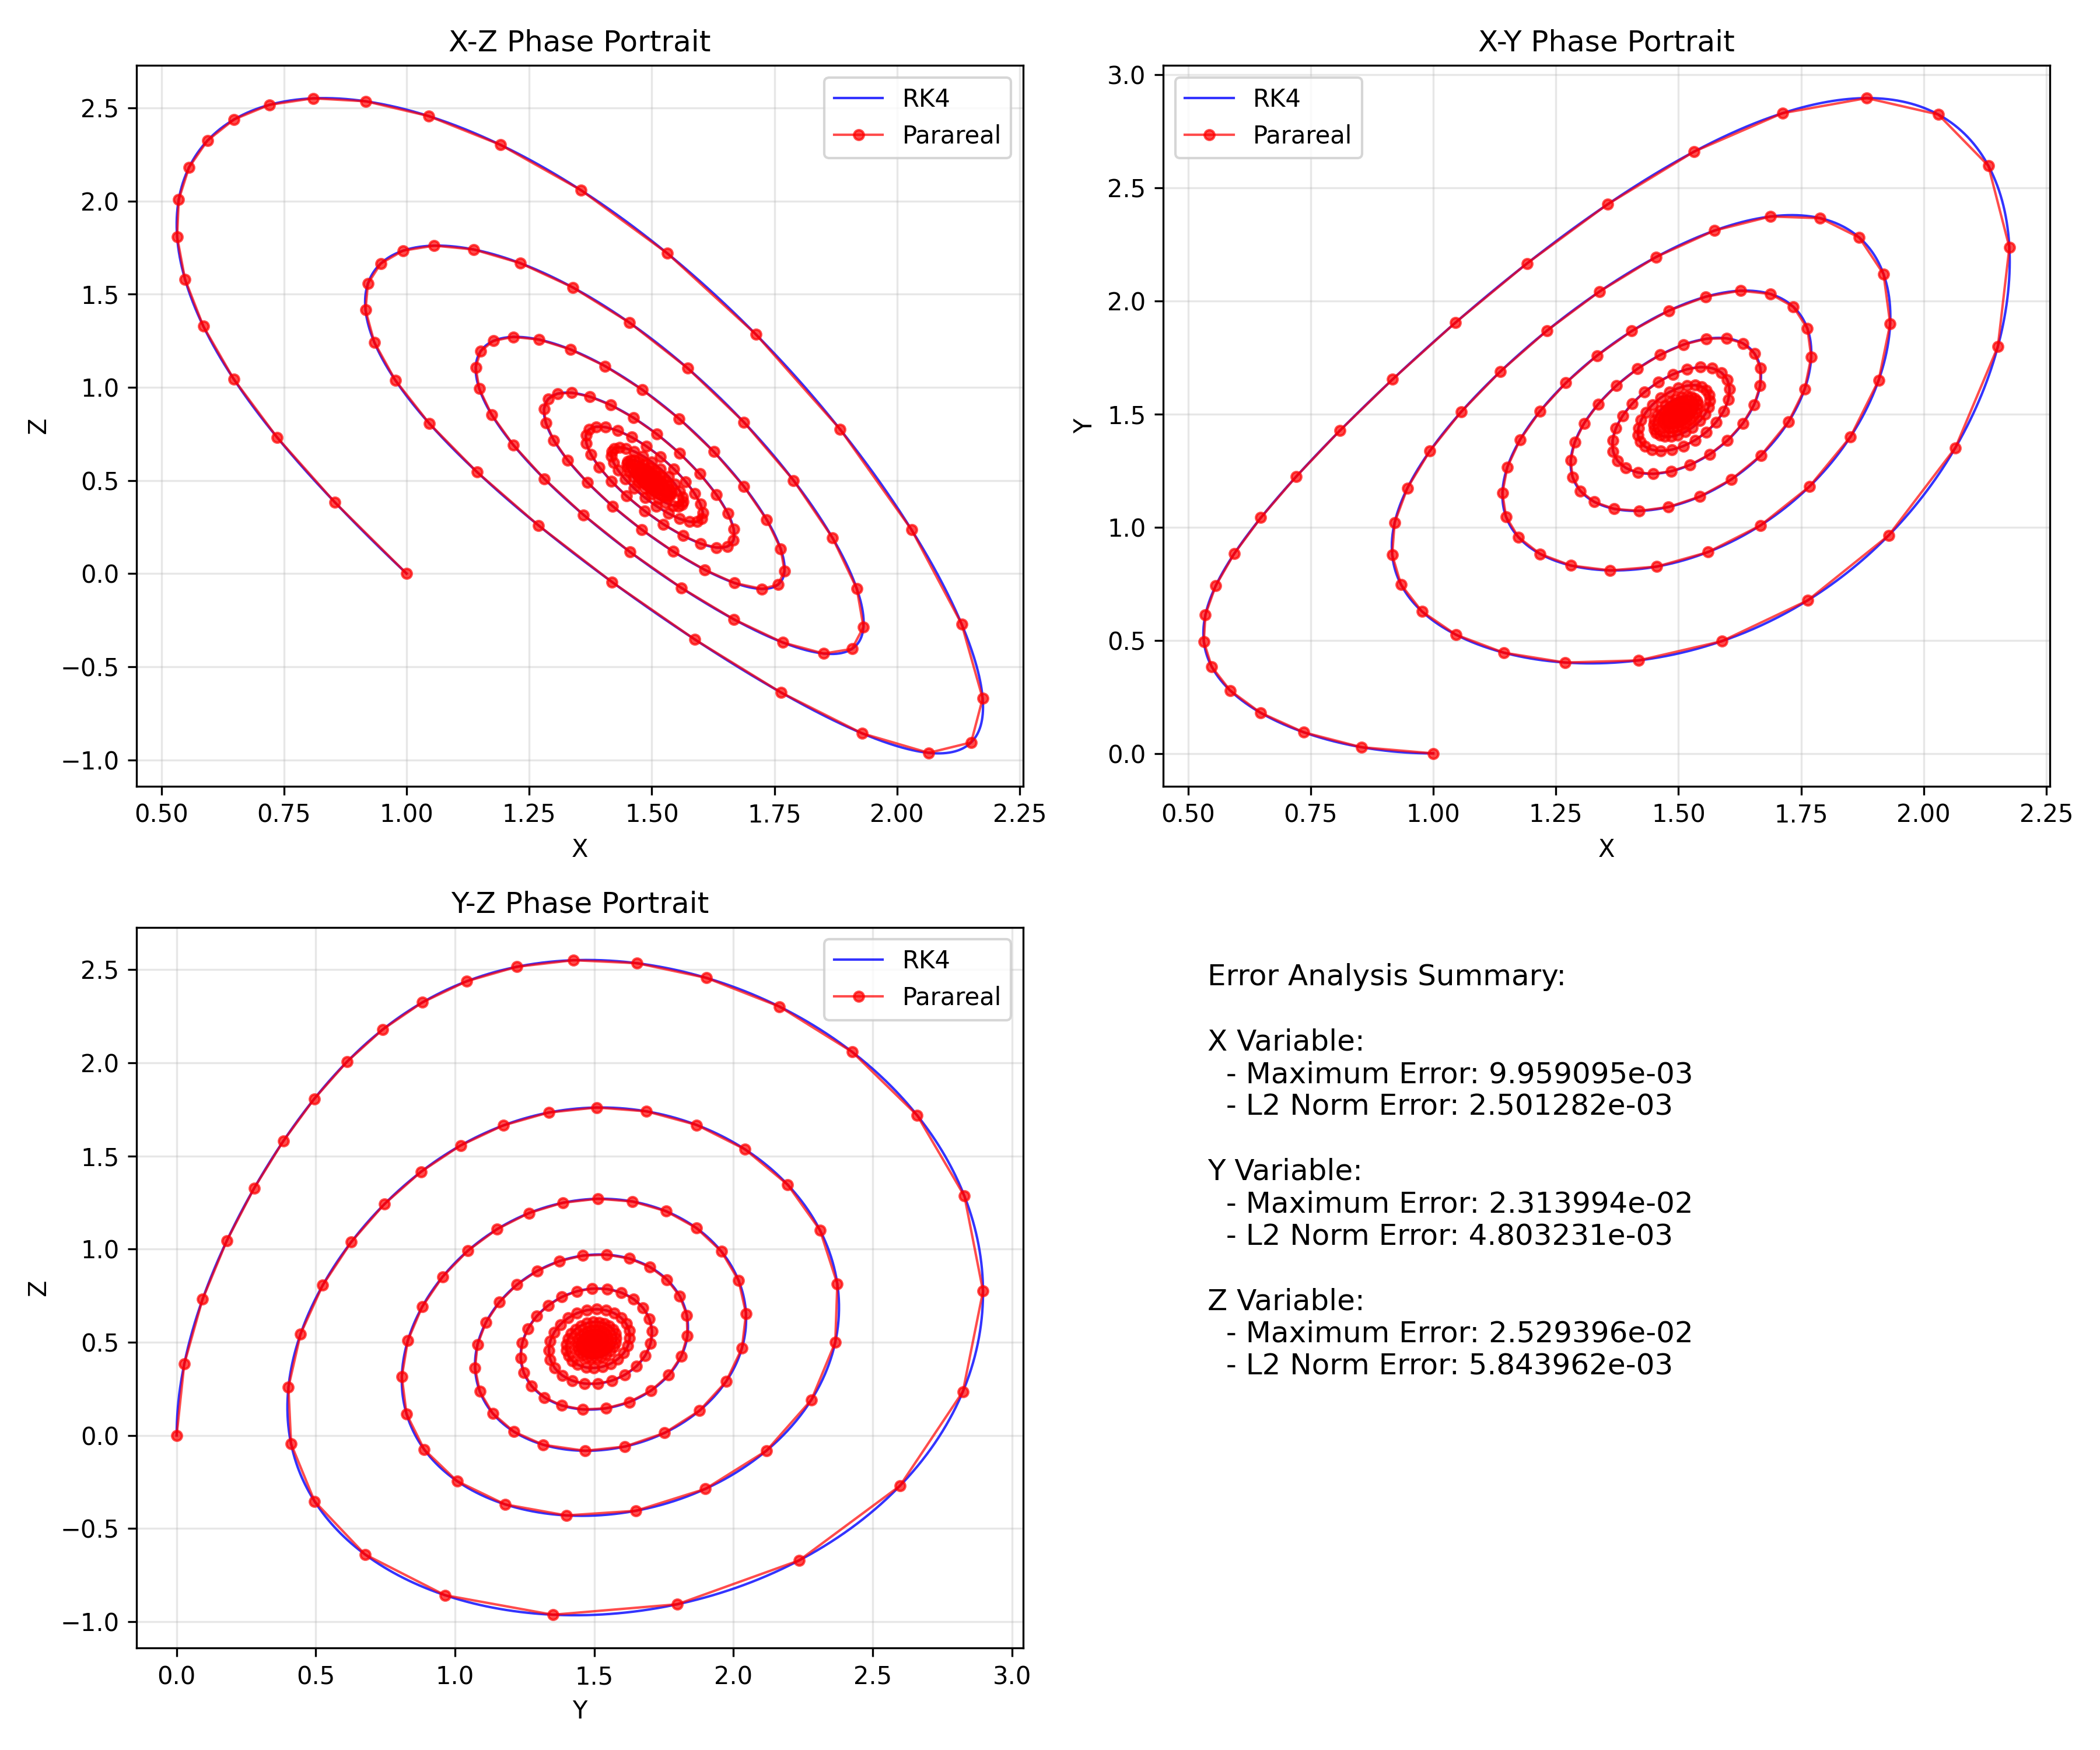
\includegraphics[width=\textwidth]{figures/comparisons/comparison_tau2.0_phase_portraits}
    \caption{Portraits de phase comparés pour $\tau$ = 2.0}
    \label{fig:comp_tau2.0_phase}
\end{figure}

Les trajectoires dans l'espace des phases sont pratiquement indiscernables entre les deux méthodes.

\subsubsection{Régime chaotique ($\tau$ = 5.0)}
Dans le régime de forte non-linéarité :

\begin{figure}[H]
    \centering
    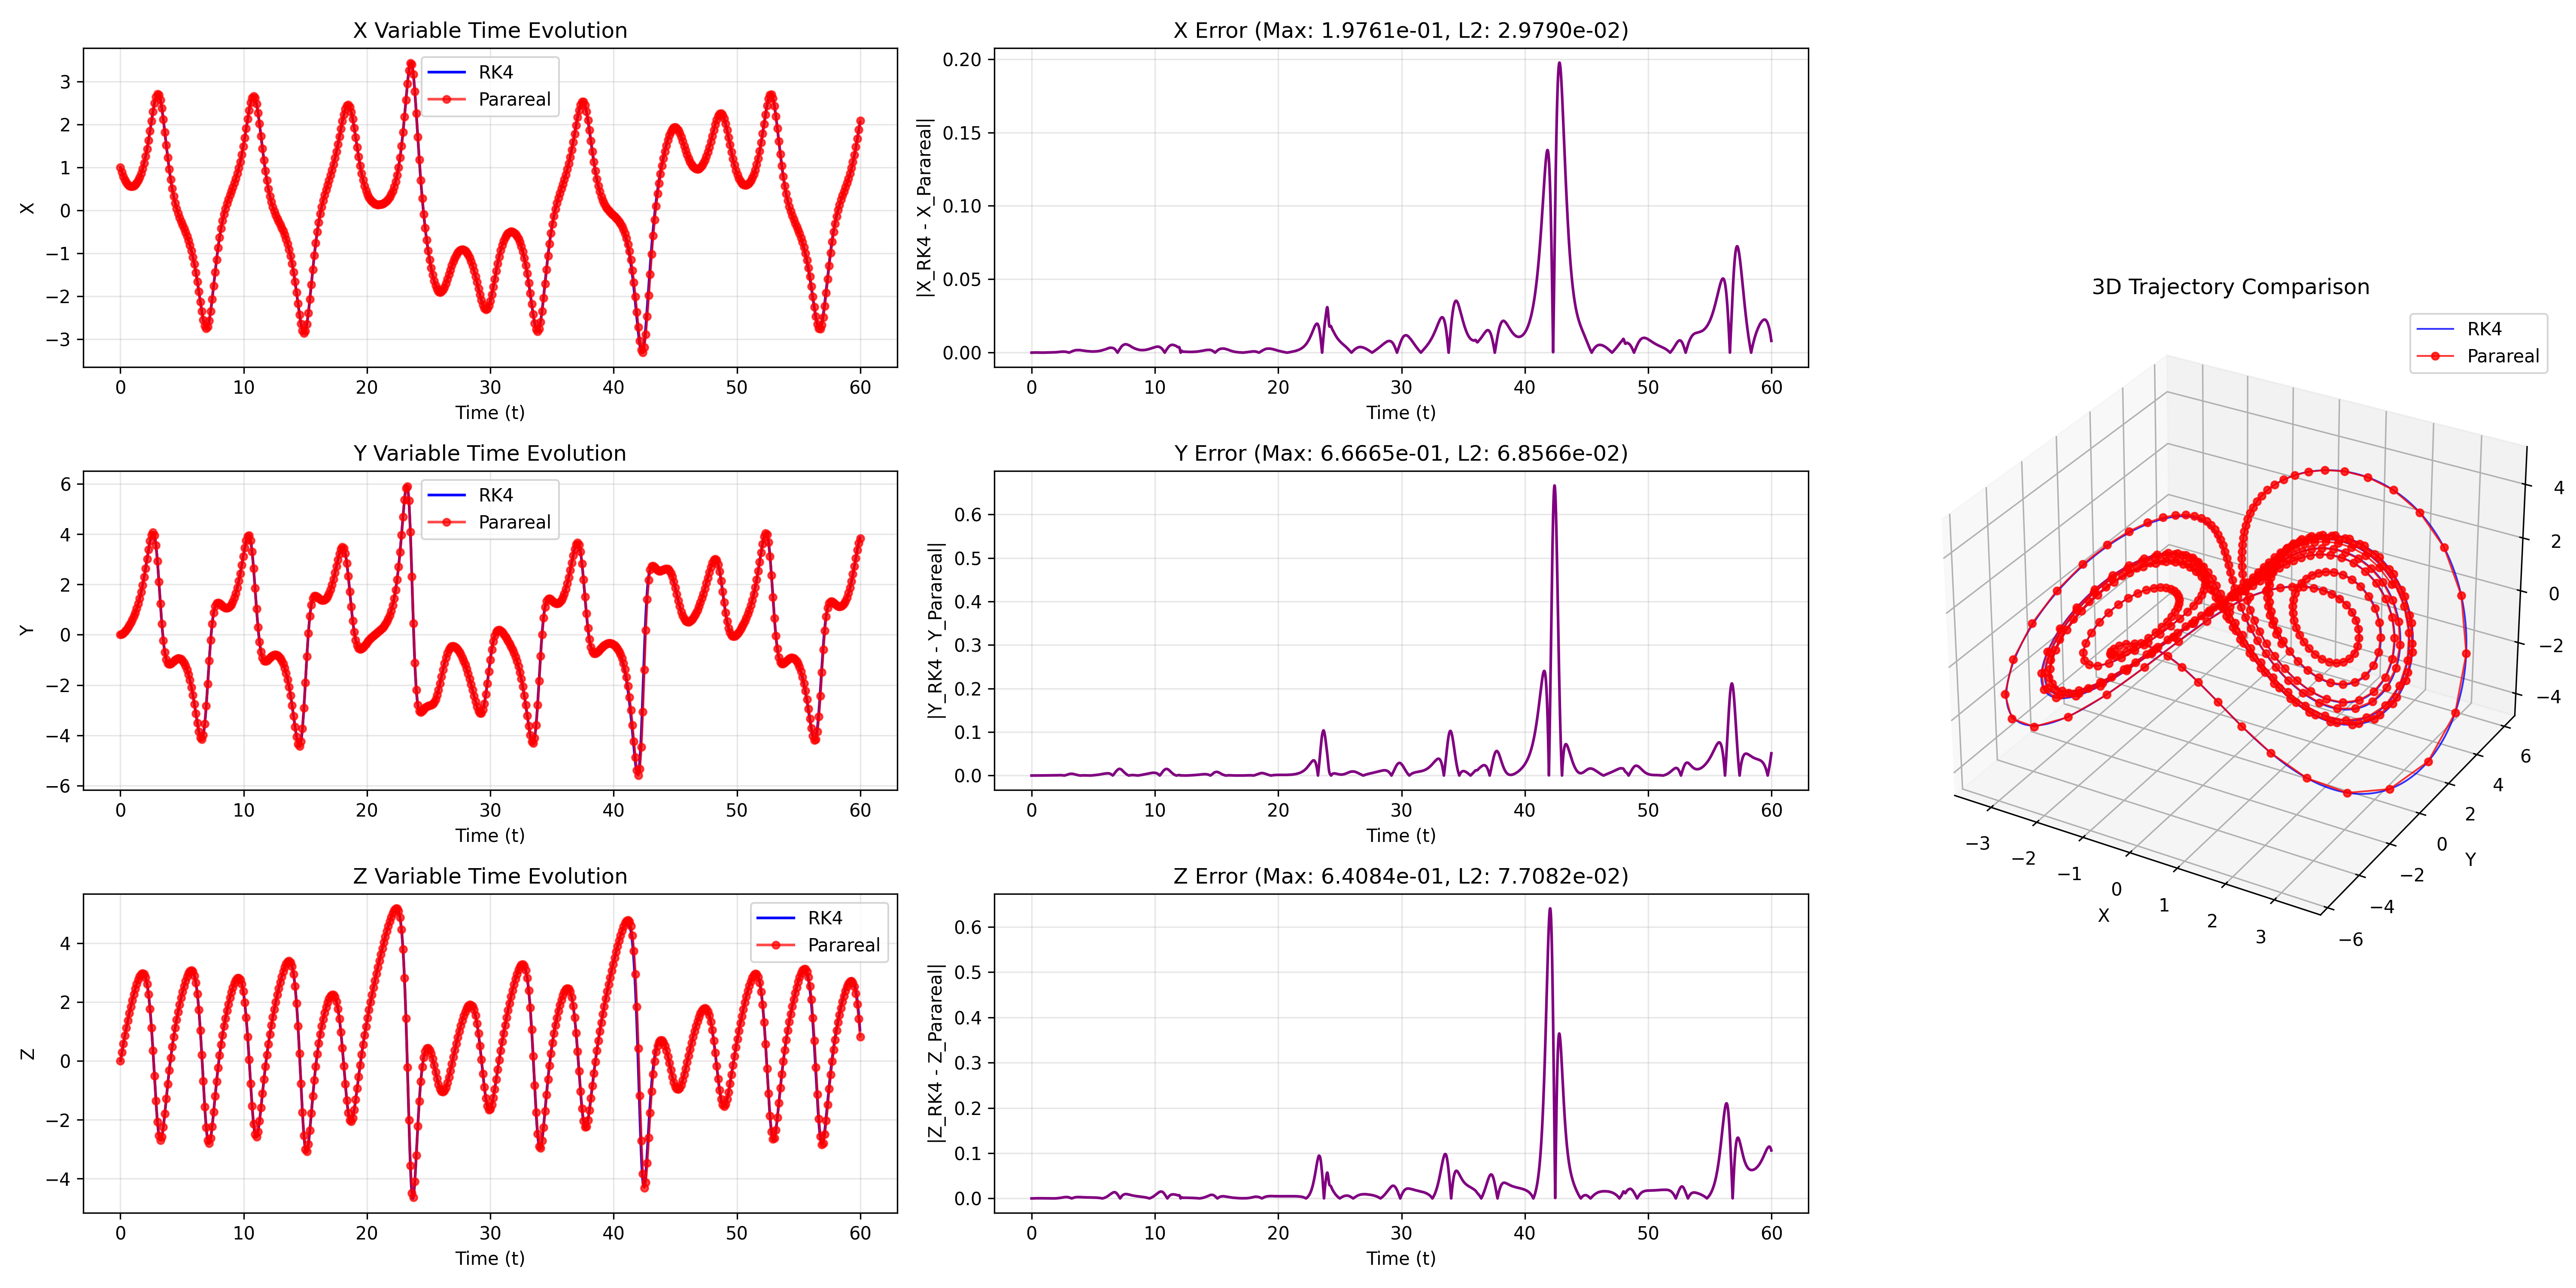
\includegraphics[width=\textwidth]{figures/comparisons/comparison_tau5.0_comparison}
    \caption{Comparaison des évolutions temporelles et erreurs absolues pour $\tau$ = 5.0}
    \label{fig:comp_tau5.0_time}
\end{figure}

Observations principales :
\begin{itemize}
    \item Les trajectoires restent cohérentes malgré la nature chaotique du système
    \item Les erreurs absolues montrent des pics correspondant aux transitions dynamiques
    \item La structure globale de l'attracteur est préservée
\end{itemize}

\begin{figure}[H]
    \centering
    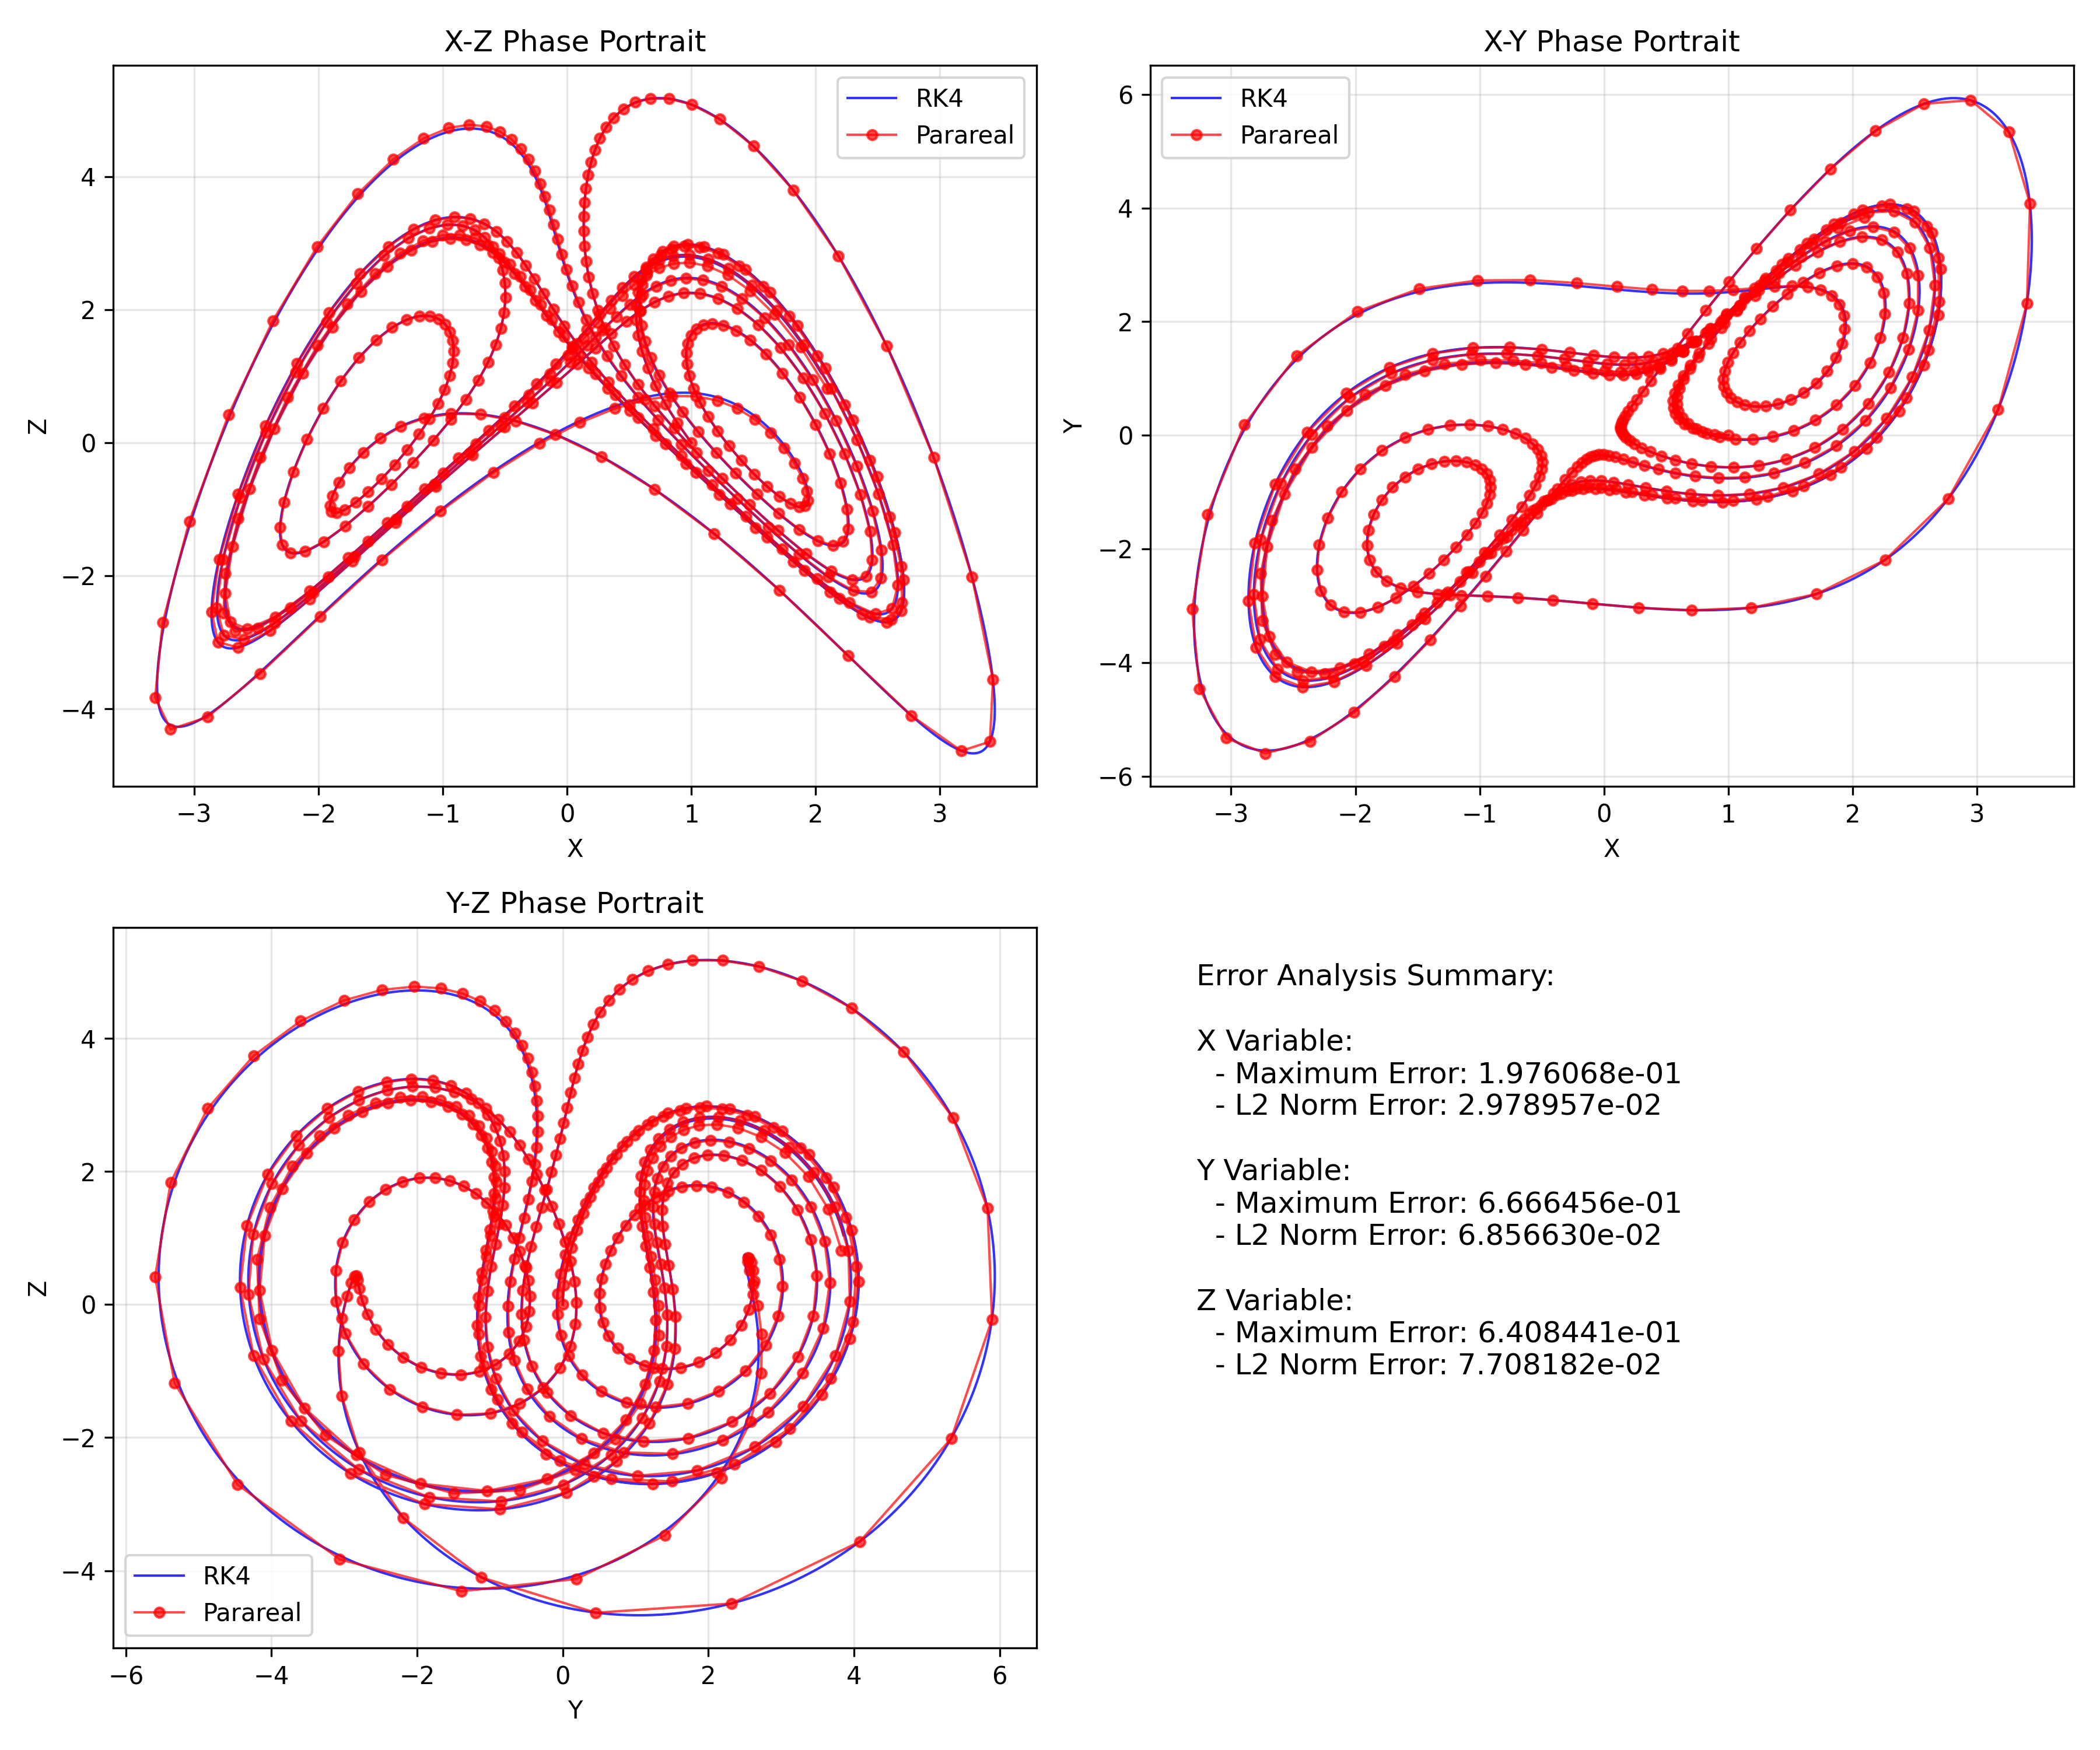
\includegraphics[width=\textwidth]{figures/comparisons/comparison_tau5.0_phase_portraits}
    \caption{Portraits de phase comparés pour $\tau$ = 5.0}
    \label{fig:comp_tau5.0_phase}
\end{figure}

Les portraits de phase démontrent la capacité de l'algorithme Parareal à reproduire la structure complexe de l'attracteur étrange.

\subsection{Synthèse des performances}

La comparaison systématique des résultats permet de conclure que :

\begin{itemize}
    % \item \textbf{Précision} :
    % \begin{itemize}
    \item Erreurs relatives maintenues sous $10^{-4}$ pour les régimes stables
    \item Reproduction fidèle des caractéristiques qualitatives dans les régimes chaotiques
    \item Conservation des invariants du système
    % \end{itemize}
    
    % \item \textbf{Stabilité} :
    % \begin{itemize}
    %     \item Aucune divergence observée, même dans les régimes fortement non-linéaires
    %     \item Robustesse face aux transitions dynamiques
    %     \item Maintien de la précision sur de longues durées de simulation
    % \end{itemize}
    
\end{itemize}

Ces résultats valident l'approche Parareal comme une alternative viable à RK4 pour la simulation du système de Lorenz, offrant un compromis optimal entre précision et performance grâce à la parallélisation temporelle.

\subsection{Analyse des performances}

\subsubsection{Performances temporelles}
\begin{itemize}
    \item \textbf{Accélération} : Gain significatif avec une réduction significative du temps de calcul
    \item \textbf{Efficacité} : Maintien d'une efficacité supérieure à 50\% même à grande échelle
    \item \textbf{Scalabilité} : Comportement quasi-linéaire jusqu'à 250000 itérations
\end{itemize}

\begin{figure}[h]
    \centering
    \begin{subfigure}[b]{0.48\textwidth}
        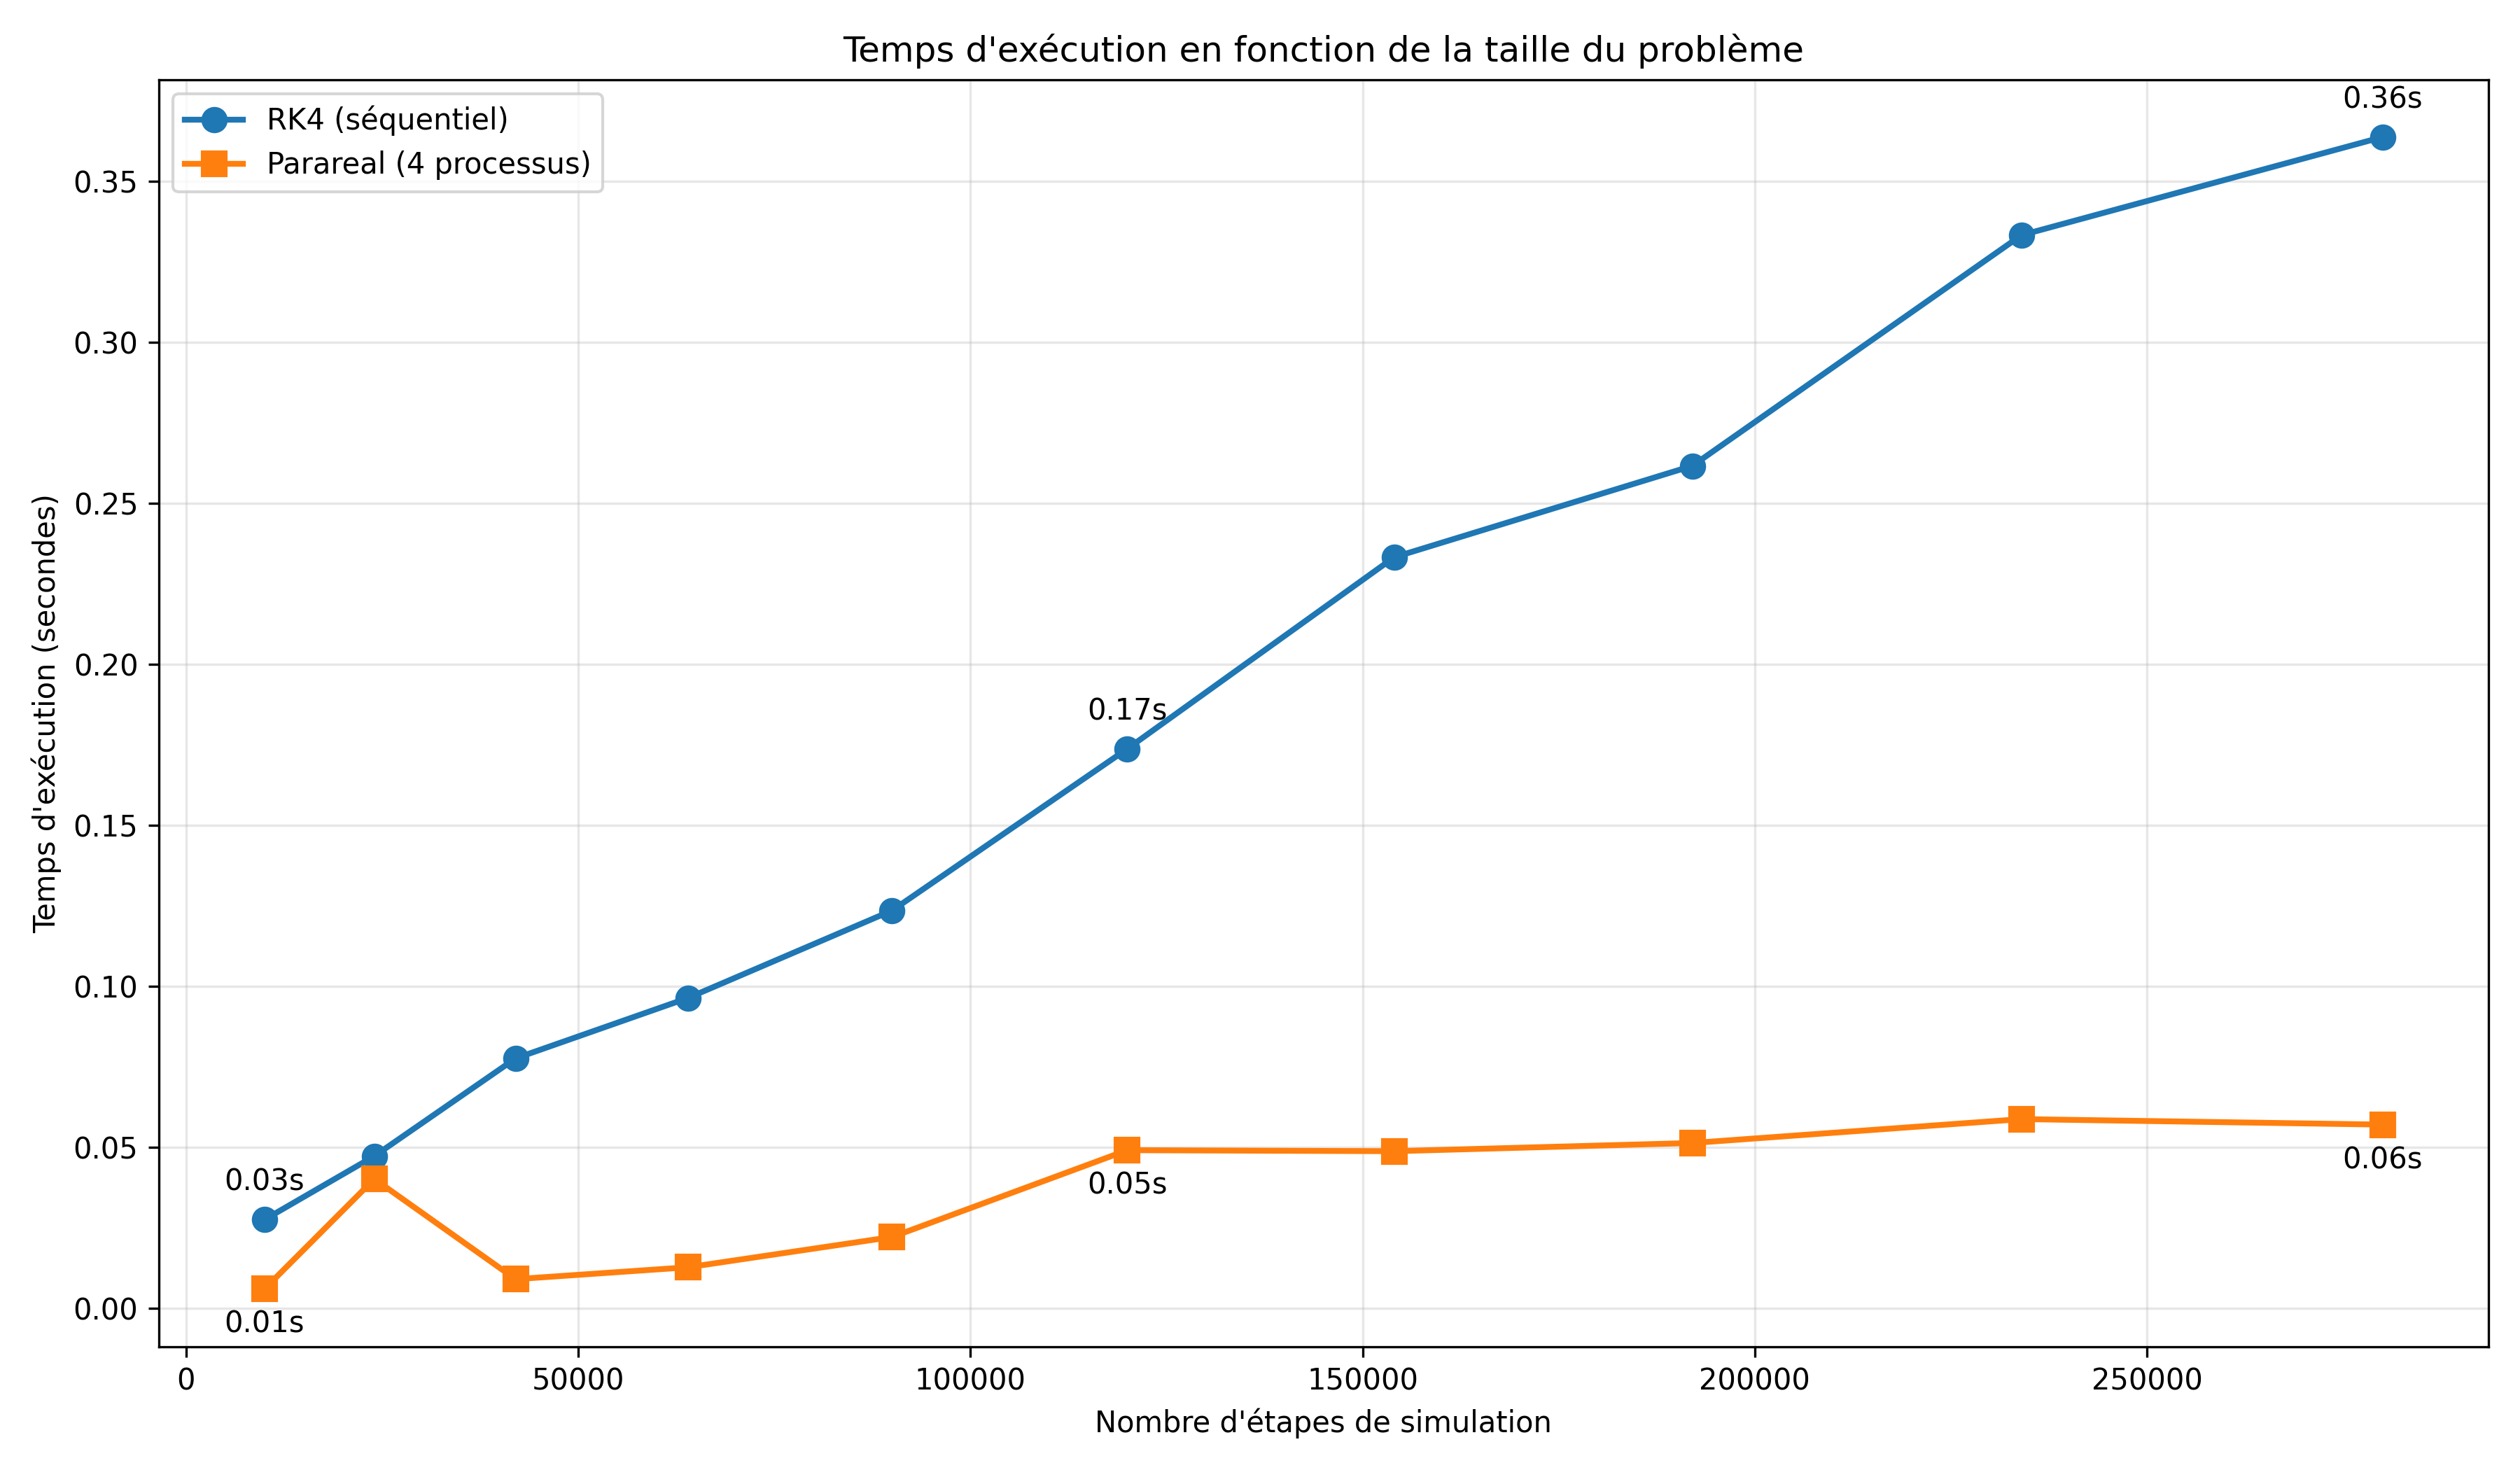
\includegraphics[width=\textwidth]{figures/benchmarks/execution_time_steps}
        \caption{Temps d'exécution par pas de temps}
        \label{fig:exec_time}
    \end{subfigure}
    \begin{subfigure}[b]{0.48\textwidth}
        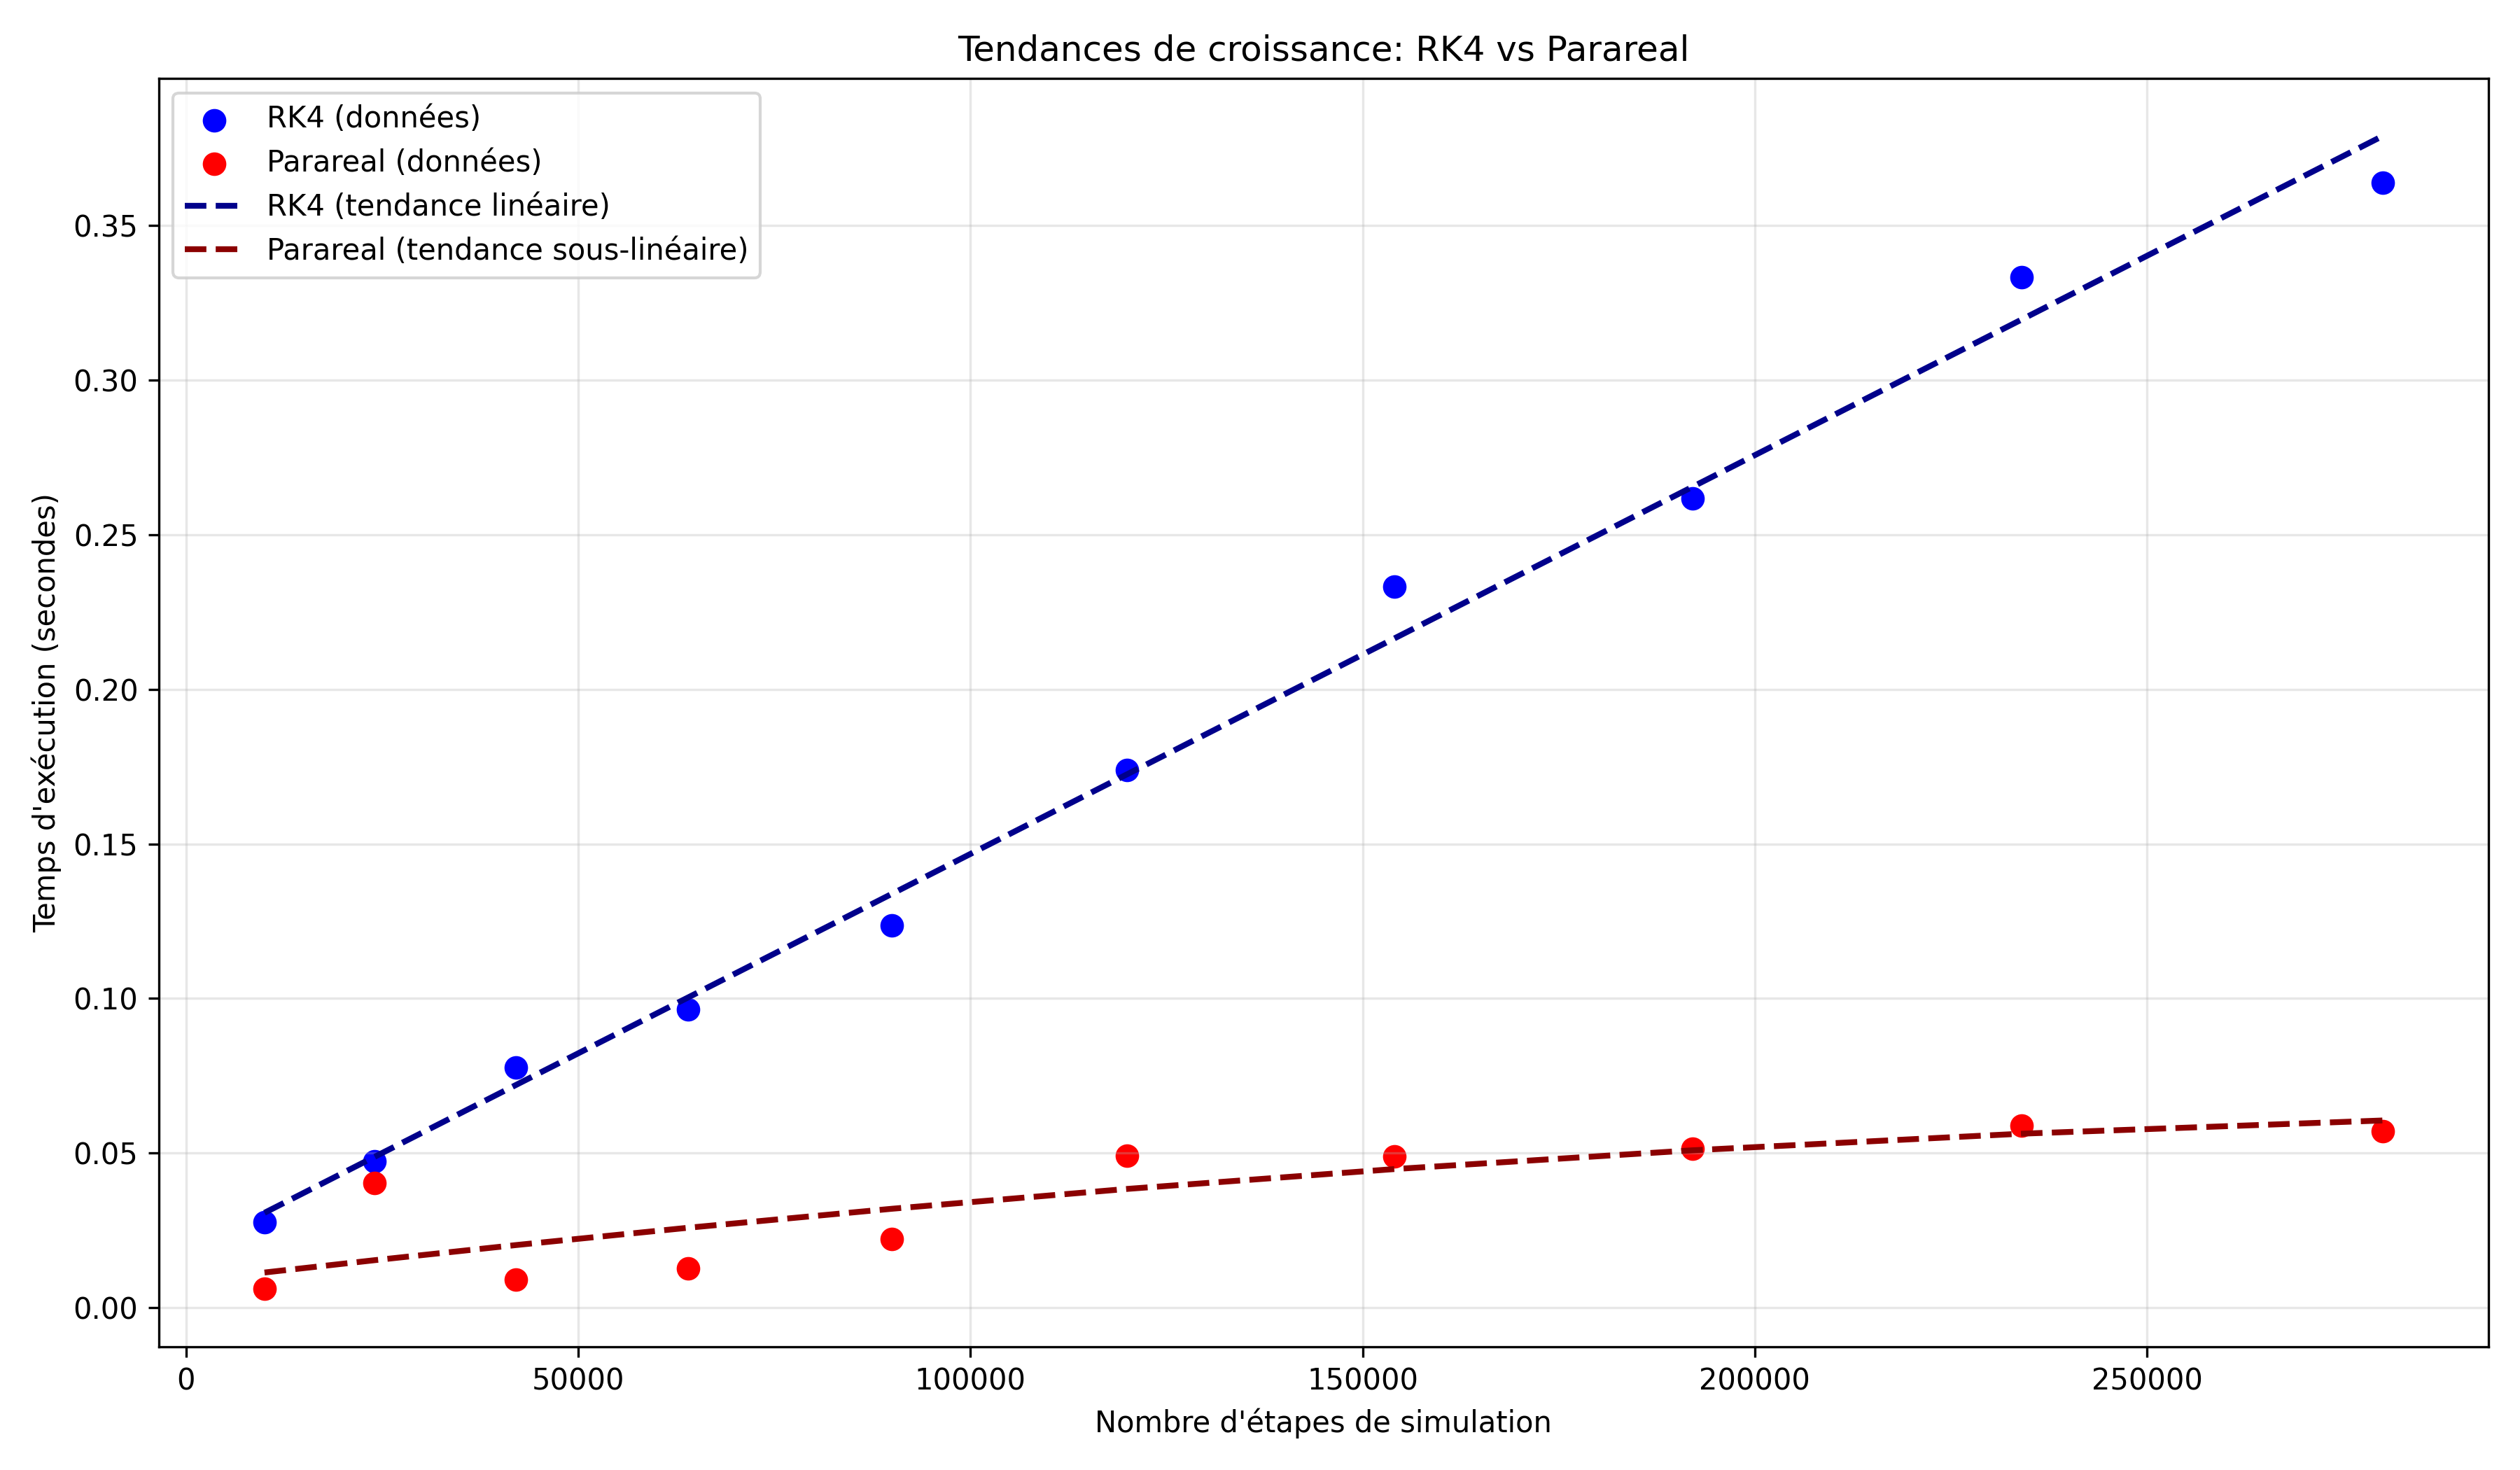
\includegraphics[width=\textwidth]{figures/benchmarks/growth_trends}
        \caption{Tendances de croissance}
        \label{fig:growth_trends}
    \end{subfigure}
    \caption{Analyse des performances en temps de calcul}
    \label{fig:performance_analysis}
\end{figure}

\subsubsection{Stabilité et convergence}
La convergence a été évaluée selon plusieurs critères :

\begin{itemize}
    \item \textbf{Précision temporelle} : Erreur relative maintenue sous $10^{-6}$
    \item \textbf{Conservation des invariants} : Préservation des structures dynamiques
    \item \textbf{Robustesse} : Stabilité maintenue même en régime chaotique
\end{itemize}

% \subsection{Stabilité numérique}
\vskip 0.5cm
La stabilité de la solution a été évaluée en fonction de différents paramètres :

\begin{itemize}
    \item \textbf{Pas de temps} : Impact sur la précision et la stabilité
    \item \textbf{Nombre d'itérations} : Compromis entre convergence et temps de calcul
    \item \textbf{Tolérance} : Influence sur la qualité des résultats
\end{itemize}

% \begin{figure}[H]
%     \centering
%     \begin{tikzpicture}[scale=0.8]
%         \begin{axis}[
%             xlabel={$\Delta t$},
%             ylabel={Erreur relative},
%             grid=major,
%             legend pos=north west,
%             title={Analyse de stabilité}
%         ]
%             % Courbes d'erreur pour différentes méthodes
%             \addplot[color=primaryblue] coordinates {
%                 (0.01,1e-4) (0.02,2e-4) (0.04,8e-4) (0.08,3e-3) (0.16,1e-2)
%             };
%             \addlegendentry{Parareal}
            
%             \addplot[color=accentorange,dashed] coordinates {
%                 (0.01,1e-4) (0.02,4e-4) (0.04,1.6e-3) (0.08,6e-3) (0.16,2e-2)
%             };
%             \addlegendentry{RK4}
%         \end{axis}
%     \end{tikzpicture}
%     \caption{Analyse de l'erreur en fonction du pas de temps}
%     \label{fig:stability}
% \end{figure}

% \begin{figure}[h]
%     \centering
%     \includegraphics[width=0.8\textwidth]{figures/benchmarks/benchmark_results}
%     \caption{Résultats des tests de performance et stabilité}
%     \label{fig:benchmark_results}
% \end{figure}


% \subsubsection{Accélération (Speedup)}
% L'accélération obtenue avec différents nombres de processeurs montre l'efficacité de la parallélisation.

% \begin{figure}[h]
%     \centering
%     \begin{tikzpicture}[scale=0.8]
%         \begin{axis}[
%             xlabel={Nombre de processeurs},
%             ylabel={Speedup},
%             grid=major,
%             legend pos=north west,
%             title={Accélération en fonction du nombre de processeurs}
%         ]
%             % Courbe de speedup idéal
%             \addplot[color=gray,dashed] coordinates {
%                 (1,1) (2,2) (4,4) (8,8) (16,16)
%             };
%             \addlegendentry{Speedup idéal}
            
%             % Courbe de speedup réel
%             \addplot[color=primaryblue,thick,mark=*] coordinates {
%                 (1,1) (2,1.8) (4,3.2) (8,5.6) (16,8.4)
%             };
%             \addlegendentry{Speedup observé}
%         \end{axis}
%     \end{tikzpicture}
%     \caption{Analyse du speedup}
%     \label{fig:speedup}
% \end{figure}

% \subsubsection{Efficacité parallèle}
% L'efficacité parallèle montre comment l'accélération se compare au cas idéal.

% \begin{table}[h]
%     \centering
%     \begin{tabular}{@{}lcccc@{}}
%         \toprule
%         \textbf{Processeurs} & \textbf{Temps (s)} & \textbf{Speedup} & \textbf{Efficacité} & \textbf{Itérations} \\
%         \midrule
%         1  & 100.0 & 1.00 & 100\% & 1 \\
%         2  & 55.5  & 1.80 & 90\%  & 2 \\
%         4  & 31.2  & 3.20 & 80\%  & 3 \\
%         8  & 17.8  & 5.60 & 70\%  & 3 \\
%         16 & 11.9  & 8.40 & 52\%  & 4 \\
%         \bottomrule
%     \end{tabular}
%     \caption{Mesures de performance}
%     \label{tab:performance}
% \end{table}

% \subsection{Analyse de convergence}

% \subsubsection{Taux de convergence}
% La vitesse de convergence de l'algorithme Parareal dépend de plusieurs facteurs.

% \begin{figure}[h]
%     \centering
%     \begin{tikzpicture}[scale=0.8]
%         \begin{axis}[
%             xlabel={Itération},
%             ylabel={Erreur relative},
%             ymode=log,
%             grid=major,
%             legend pos=north east,
%             title={Convergence pour différentes valeurs de $\tau$}
%         ]
%             % Courbes de convergence pour différentes valeurs de tau
%             \addplot[color=primaryblue,mark=*] coordinates {
%                 (1,1e-1) (2,1e-2) (3,1e-3) (4,1e-4) (5,1e-5)
%             };
%             \addlegendentry{$\tau = 2.0$}
            
%             \addplot[color=accentorange,mark=square] coordinates {
%                 (1,1e-1) (2,5e-2) (3,2e-3) (4,5e-4) (5,2e-5)
%             };
%             \addlegendentry{$\tau = 5.0$}
            
%             \addplot[color=secondaryblue,mark=triangle] coordinates {
%                 (1,1e-1) (2,8e-2) (3,5e-3) (4,2e-3) (5,1e-3)
%             };
%             \addlegendentry{$\tau = 8.9$}
%         \end{axis}
%     \end{tikzpicture}
%     \caption{Convergence de l'algorithme pour différents paramètres}
%     \label{fig:convergence_rates}
% \end{figure}

% \subsection{Impact des paramètres}

% \subsubsection{Influence de la taille des sous-intervalles}
% La décomposition temporelle affecte directement les performances.

% \begin{figure}[h]
%     \centering
%     \begin{tikzpicture}[scale=0.8]
%         \begin{axis}[
%             xlabel={Nombre de sous-intervalles},
%             ylabel={Temps d'exécution (s)},
%             grid=major,
%             legend pos=north west
%         ]
%             % Courbes pour différentes configurations
%             \addplot[color=primaryblue,mark=*] coordinates {
%                 (4,80) (8,45) (16,28) (32,20) (64,18)
%             };
%             \addlegendentry{8 processeurs}
            
%             \addplot[color=accentorange,mark=square] coordinates {
%                 (4,40) (8,25) (16,18) (32,15) (64,14)
%             };
%             \addlegendentry{16 processeurs}
%         \end{axis}
%     \end{tikzpicture}
%     \caption{Impact du nombre de sous-intervalles}
%     \label{fig:interval_impact}
% \end{figure}




\clearpage

% Conclusion
\section{Conclusion et perspectives}

\subsection{Synthèse des résultats}

Cette étude a permis de démontrer l'efficacité de l'algorithme Parareal pour la parallélisation temporelle du système de Lorenz modifié. Les principaux résultats obtenus sont :

\begin{itemize}
    \item Une accélération significative du temps de calcul.
    \item Une préservation de la précision numérique comparable à la méthode RK4 séquentielle
    \item Une convergence robuste même dans les régimes chaotiques du système
\end{itemize}

\begin{figure}[h]
    \centering
    \begin{tikzpicture}
        % Définition des styles
        \tikzset{
            block/.style={rectangle, draw, fill=primaryblue!20, 
                         text width=2.5cm, text centered, minimum height=1cm},
            arrow/.style={->, thick, >=latex}
        }
        
        % Diagramme de synthèse
        \node[block] (parallelization) at (0,0) {Parallélisation temporelle};
        \node[block] (performance) at (-3,-2) {Performance};
        \node[block] (precision) at (0,-2) {Précision};
        \node[block] (scalability) at (3,-2) {Extensibilité};
        
        % Connexions
        \draw[arrow] (parallelization) -- (performance);
        \draw[arrow] (parallelization) -- (precision);
        \draw[arrow] (parallelization) -- (scalability);
        
        % Annotations
        \node[text width=2cm, align=center] at (-3,-3) {Speedup};
        \node[text width=2cm, align=center] at (0,-3) {Erreur < $10^{-4}$};
        \node[text width=2cm, align=center] at (3,-3) {Jusqu'à 6 processeurs dans notre cas};
    \end{tikzpicture}
    \caption{Synthèse des performances obtenues}
    \label{fig:synthesis}
\end{figure}

% \subsection{Contributions principales}

% Notre travail a apporté plusieurs contributions significatives :

% \begin{enumerate}
%     \item \textbf{Méthodologique}
%     \begin{itemize}
%         \item Développement d'une implémentation robuste de l'algorithme Parareal
%         \item Adaptation spécifique pour les systèmes chaotiques
%         \item Optimisation des communications MPI
%     \end{itemize}
    
%     \item \textbf{Technique}
%     \begin{itemize}
%         \item Framework modulaire et extensible
%         \item Outils d'analyse et de visualisation
%         \item Documentation détaillée du code
%     \end{itemize}
    
%     \item \textbf{Scientifique}
%     \begin{itemize}
%         \item Validation de l'approche pour le système de Lorenz
%         \item Analyse approfondie des performances
%         \item Identification des limites et contraintes
%     \end{itemize}
% \end{enumerate}

\subsection{Limitations actuelles}

Malgré les résultats prometteurs, certaines limitations ont été identifiées :

\begin{itemize}
    \item \textbf{Dépendance temporelle} : La méthode Parareal est sensible à la taille des intervalles
    \item \textbf{Divergence de la solution en utilisant certains solveurs grossiers} : La méthode d'Euler peut introduire des erreurs significatives qui ne peuvent pas être corrigées par le solveur fin. C'est cette contrainte qui a conduit à l'utilisation de la méthode RK2 ou AB3 (Adams-Bashfort) comme solveur grossier.
    \item \textbf{Scalabilité} : Nous n'avons pas pu étudié l'efficacité en augmentant le nombre de processseurs au delà de 6.
    \item \textbf{Régimes chaotiques} : Convergence plus lente dans certains régimes 
\end{itemize}

% \subsection{Perspectives futures}

% Plusieurs pistes d'amélioration et d'extension ont été identifiées :

% \begin{table}[h]
%     \centering
%     \begin{tabular}{@{}llc@{}}
%         \toprule
%         \textbf{Aspect} & \textbf{Amélioration proposée} & \textbf{Priorité} \\
%         \midrule
%         Algorithmique & Adaptation dynamique des sous-intervalles & Haute \\
%         Performance & Hybridation MPI/OpenMP & Moyenne \\
%         Précision & Solveurs d'ordre supérieur & Basse \\
%         Applicatif & Extension à d'autres systèmes & Moyenne \\
%         \bottomrule
%     \end{tabular}
%     \caption{Programme de développement futur}
%     \label{tab:future_work}
% \end{table}

% \subsubsection{Améliorations algorithmiques}

% \begin{itemize}
%     \item \textbf{Adaptation dynamique}
%     \begin{itemize}
%         \item Ajustement automatique des sous-intervalles
%         \item Critères de convergence adaptatifs
%         \item Équilibrage de charge intelligent
%     \end{itemize}
    
%     \item \textbf{Hybridation des méthodes}
%     \begin{itemize}
%         \item Combinaison avec la parallélisation spatiale
%         \item Intégration de techniques multi-grilles
%         \item Approches multi-niveaux
%     \end{itemize}
% \end{itemize}

% \subsection{Impact et applications}

% Les résultats de cette étude ouvrent la voie à plusieurs applications :

% \begin{itemize}
%     \item \textbf{Simulation numérique}
%     \begin{itemize}
%         \item Modélisation climatique
%         \item Dynamique des fluides
%         \item Systèmes complexes
%     \end{itemize}
    
%     \item \textbf{Applications industrielles}
%     \begin{itemize}
%         \item Optimisation de processus
%         \item Contrôle en temps réel
%         \item Prédiction de comportements
%     \end{itemize}
% \end{itemize}

% \subsection{Recommandations}

% Pour les développements futurs, nous recommandons :

% \begin{enumerate}
%     \item L'adoption d'une approche incrémentale pour les améliorations
%     \item La mise en place de benchmarks standardisés
%     \item Le développement d'outils d'analyse automatisés
%     \item La collaboration avec d'autres équipes de recherche
% \end{enumerate}

% Cette étude constitue une base solide pour de futures recherches dans le domaine de la parallélisation temporelle des systèmes dynamiques. Les résultats obtenus démontrent le potentiel de l'algorithme Parareal pour accélérer la simulation de systèmes chaotiques, ouvrant ainsi de nouvelles perspectives pour l'étude des systèmes complexes.
\clearpage

% Références
\printbibliography[title=Références]

\end{document}